\documentclass[11pt]{article}

% ========================= En-Tête ======================= %
% --- Packages --- %
\usepackage[T1]{fontenc}
\usepackage[utf8]{inputenc}
\usepackage{graphicx}
\usepackage[french]{babel}
\usepackage[margin=2.5cm]{geometry}
\usepackage{amsmath, amssymb}
\usepackage{enumitem}
\usepackage{xcolor}
\usepackage{titlesec}
\usepackage{mdframed}
\usepackage{algorithm}
\usepackage{algpseudocode}
\usepackage{float}
\usepackage{forest}
\usepackage{array}
\usepackage{dirtree}
\usepackage{cancel}
\usepackage{hyperref}
\usepackage{float}


% Configuration biblatex
\usepackage[
    backend=biber,
    style=numeric,    
    sorting=none 
]{biblatex}

\addbibresource{biblio.bib}  % Fichier .bib

\pagestyle{empty}

% --- Envs --- %
\newenvironment{avantpropos}{%
    \begin{mdframed}[
        linecolor=sectioncolor!40,
        linewidth=0.8pt,
        backgroundcolor=sectioncolor!5,
        innerleftmargin=10pt,
        innerrightmargin=10pt,
        innertopmargin=6pt,
        innerbottommargin=6pt,
        skipabove=8pt,
        skipbelow=8pt
    ]
    \noindent\textbf{\small\color{sectioncolor}}\enspace\small\itshape
}{%
    \end{mdframed}
}

\newenvironment{paraph}[1]{%
  \medskip
  \noindent\textbf{#1.}\quad

  \vspace{0.2cm}
}{%
  \medskip
}

\newenvironment{remarque}{%
    \begin{mdframed}[
        linecolor=sectioncolor!40,
        linewidth=0.8pt,
        backgroundcolor=sectioncolor!5,
        innerleftmargin=10pt,
        innerrightmargin=10pt,
        innertopmargin=6pt,
        innerbottommargin=6pt,
        skipabove=8pt,
        skipbelow=8pt
    ]
    \noindent\textbf{\small\color{sectioncolor}Remarque.}\enspace\small\itshape
}{%
    \end{mdframed}
}

% Couleurs personnalisées
\definecolor{sectioncolor}{RGB}{50, 70, 120}
\definecolor{subsectioncolor}{RGB}{80, 80, 80}

% --- Règles --- %
\algrenewcommand\algorithmicprocedure{\textbf{Procédure}}
\algrenewcommand\algorithmicfunction{\textbf{Fonction}}
\algrenewcommand\algorithmicif{\textbf{Si}}
\algrenewcommand\algorithmicthen{\textbf{alors}}
\algrenewcommand\algorithmicelse{\textbf{Sinon}}
\algrenewcommand\algorithmicfor{\textbf{Pour}}
\algrenewcommand\algorithmicforall{\textbf{Pour tout}}
\algrenewcommand\algorithmicdo{\textbf{faire}}
\algrenewcommand\algorithmicwhile{\textbf{Tant que}}
\algrenewcommand\algorithmicreturn{\textbf{Retourner}}
\algrenewcommand\algorithmicrepeat{\textbf{Répéter}}
\algrenewcommand\algorithmicuntil{\textbf{Jusqu'à}}
\algrenewtext{EndIf}{\textbf{Fin si}}
\algrenewtext{EndFor}{\textbf{Fin pour}}
\algrenewtext{EndWhile}{\textbf{Fin tant que}}
\algrenewtext{EndProcedure}{\textbf{Fin procédure}}
\algrenewtext{EndFunction}{\textbf{Fin fonction}}
\algdef{SE}[TRY]{Try}{EndTry}{\textbf{Essayer}}{\textbf{Fin essayer}}
\algdef{C}[TRY]{TRY}{Catch}[1]{\textbf{Capturer} #1}    

\titleformat{\section}[hang]{\Large\bfseries}{\thesection.}{0.5em}{}
\titleformat{\subsection}[hang]{\large\bfseries}{\thesubsection.}{0.5em}{}
\titleformat{\subsubsection}[hang]{\large\bfseries}{\thesubsubsection.}{0.5em}{}
\renewcommand{\theHsubsection}{\thesection.\thesubsection}

% ========================= Corps ======================= %
\begin{document}
\begin{titlepage}
    \begin{center}
        \begin{minipage}[c]{0.45\textwidth}
            \centering
            
\includegraphics[width=0.30\linewidth]{img/logo_LORIA.png}
        \end{minipage}
        \rule{1pt}{2.2cm}
        \begin{minipage}[c]{0.45\textwidth}
            \centering
            
\includegraphics[width=0.6\linewidth]{img/logo_UL.png}
        \end{minipage}
    \end{center}

    \vspace{1cm} % Espace vertical après les logos
    \vspace*{\fill}

    \begin{center}
        \textbf{\Huge Structures de données pour l’unification en logique du premier ordre} \\
        \vspace{0.5cm}
        \Large Rapport en vue de la validation de l’UE Initiation à la recherche \\
        \vspace{0.5cm}
        Année universitaire 2025-2026
    \end{center}

    \vspace*{\fill}

    % Noms auteurs :
    \begin{minipage}[t]{0.45\textwidth}
        \begin{flushleft}
            \small Etudiants~: \\
            \hspace*{1.5em} Ayath ABOGOUNRIN \\
            \hspace*{1.5em} Guillaume POTEL \\
            \hspace*{1.5em} Matheo VIGNERES
        \end{flushleft}
    \end{minipage}%
    % Barre séparatrice auteurs / encadrants :
    \begin{minipage}[t]{0.1\textwidth}
        \vspace*{0.5em} % Ajustement vertical pour aligner la barre
        \centering
        \rule{1pt}{\dimexpr3\baselineskip+ 0.5em} % Ajustement précis de la hauteur
    \end{minipage}%
    % Noms encadrants :
    \begin{minipage}[t]{0.45\textwidth}
        \begin{flushright}
            \small Encadrants : \\
            \hspace*{0pt}\llap{\hspace*{1.5em}} Julie CAILLER \\
            \hspace*{0pt}\llap{\hspace*{1.5em}} Marie DUFLOT-KREMER \\
            \hspace*{0pt}\llap{\hspace*{1.5em}} Engel LEFAUCHEUX
        \end{flushright}
    \end{minipage}
\end{titlepage}
\thispagestyle{empty}

% Page vide :
\newpage
\null

% Decharge de resp :
\newpage
\addtocontents{toc}{\setcounter{tocdepth}{-2}}  % Ne pas afficher dans sommaire
\section*{DÉCHARGE DE RESPONSABILITÉS}
\vspace*{\fill}
\textit{« L’Université de Lorraine n’entend donner ni approbation ni improbation aux opinions émises dans ce
rapport, ces opinions devant être considérées comme propres à leur auteur. »}
\vspace*{\fill}

% Remerciements : 
\newpage
\section*{REMERCIEMENTS}
Nous tenons à remercier toutes les personnes qui ont contribué au bon déroulement de notre projet
et qui nous ont aidé dans la rédaction de ce rapport.

Tout d'abord, nous voulons remercier chaleureusement l'ensemble de nos encadrants pour leur bienveillance,
leur pédagogie, leur temps et surtout leur bonne humeur tout au long du projet. 
Nous remercions donc Madame Julie Cailler, pour son soutien émotionnel sans faille, spécifiquement
face aux Discrimination Trees, Madame Marie Duflot-Kremer pour ses remarques toujours pertinentes et son
choix judicieux de date d'anniversaire, nous ayant permis de profiter d'un délicieux goûter, et enfin Monsieur Engel Lefaucheux
pour ses précieux conseils, notamment pour les benchmarks finaux, et ses propositions
hebdomadaires de chocolats qui, nous tenons à le préciser au lecteur, ont toujours été refusées.

Aussi, nous souhaitons remercier Monsieur Didier Galmiche, notre professeur de Logique cette année,
sans qui notre choix de sujet ne se serait sûrement jamais porté sur cette thématique passionnante, challegeante
et pleine de (bons comme mauvais) rebondissements. 

Enfin, nous remercions toutes les personnes nous ayant conseillé et relu lors de la rédaction
de ce rapport.



% Sommaire :
\newpage
\tableofcontents                                % Ecrit la table des matières
\newpage
\pagestyle{plain}
\setcounter{page}{1}                            % On commence à compter les pages
\addtocontents{toc}{\setcounter{tocdepth}{3}}   % On recommence à afficher dans sommaire

\phantomsection
\addcontentsline{toc}{section}{Introduction}  
\section*{Introduction}                         % On ne le numérote pas                                                  
% Paragraphe 1 : Mise en abime du sujet
En informatique, le choix des \textbf{structures de données} est une décision 
fondamentale~: elle conditionne directement l'efficacité des algorithmes qui 
les manipulent. Ce principe, universel en programmation, prend une dimension 
particulière dans le domaine de la \textbf{logique}, où la représentation 
des objets manipulés doit non seulement refléter fidèlement une syntaxe 
formelle stricte, mais aussi permettre un traitement automatique 
efficace. C'est précisément ce défi qui est au cœur de ce rapport.

\vspace{0.5cm}
% Paragraphe 2 : Définitions des notions clés
La \textbf{logique du premier ordre} est un langage formel permettant d'exprimer 
des propriétés et des relations sur des objets. Elle repose sur des expressions 
symboliques appelées \textbf{termes}, construits à partir de \textbf{variables}, 
de \textbf{constantes} et de \textbf{symboles de fonction}. Ces termes constituent 
la brique de base des \textbf{formules logiques}, et leur manipulation efficace 
est un enjeu central dans de nombreux systèmes automatiques. Parmi les opérations 
fondamentales sur ces termes, l'\textbf{unification} occupe une place de choix~: 
elle consiste à déterminer s'il existe une \textbf{substitution} de variables 
permettant de rendre deux termes identiques. Cette opération intervient notamment 
dans les \textbf{moteurs d'inférence}, les \textbf{systèmes de réécriture de termes} 
et les \textbf{prouveurs de théorèmes automatiques}.

\vspace{0.5cm}
% Paragraphe 3 : Présentation de la problématique
Dans ce contexte, une question naturelle se pose~: quelles sont les 
\textbf{structures de données} les plus adaptées pour représenter et manipuler 
efficacement des termes dans le cadre de l'unification~? Le choix d'une structure 
impactant directement l'efficacité des algorithmes qui l'exploitent, nous nous 
interrogerons également sur les \textbf{algorithmes d'unification} les mieux 
adaptés à chaque représentation. C'est autour de cette double problématique, 
structures et algorithmes, que s'articule ce travail de recherche.


\vspace{0.5cm}
% Paragraphe 4 : Annonce du plan
Nous commencerons par établir les \textbf{généralités} nécessaires à la 
compréhension du sujet~: logique des propositions, logique du premier ordre, 
preuve automatisée et unification. Nous présenterons ensuite les 
\textbf{structures de données} retenues pour représenter les termes et les 
organiser en base, ainsi que les \textbf{algorithmes d'unification} étudiés, 
en particulier le \textbf{discrimination tree}. Enfin, nous exposerons les 
\textbf{résultats expérimentaux} obtenus lors de nos benchmarks, avant de 
conclure sur les enseignements tirés de cette étude. L'ensemble du code source 
est disponible dans le dépôt git du projet~: \url{https://github.com/Metheor31Game/M1-recherche}.

\newpage
\section{Généralités}
\begin{avantpropos}
    D'après nos connaissances, l'UE de L3 intitulée \emph{Logique des propositions - Logique du premier ordre}, de Jean Lieber~\cite{lieber2024cours} et l'UE de M1 intitulée \emph{Logiques et Modèles de Calcul}, de Didier Galmiche.
\end{avantpropos}

\begin{paraph}{Fil conducteur}
Tout au long de ce chapitre, nous allons construire progressivement les outils nécessaires 
pour répondre à une question concrète : comment une machine peut-elle \emph{démontrer} 
automatiquement que «~Socrate est mortel~» d'après les hypothèses «~Tout homme est mortel.~» 
et «~Socrate est un homme~» ? Ce raisonnement, connu sous le nom de \textit{syllogisme}, 
peut sembler trivial au lecteur mais requiert,  pour être mécanisé, des outils formels précis. 
Nous introduirons d'abord brièvement la logique des propositions, sur laquelle s'appuie la 
logique du premier ordre, avant de présenter cette dernière puis l'unification, 
les deux notions centrales de ce rapport.
\end{paraph}
\subsection{Logique des propositions}
\begin{paraph}{Définition}
La \textit{logique des propositions} (ou logique propositionnelle) repose 
sur une idée simple~: on représente des \textit{faits élémentaires}, 
par exemple «~Socrate est un homme~», auxquels on attribue une 
\textit{valeur de vérité} ($vrai$ ou $faux$). Ces \textit{faits élémentaires} 
sont appelés \textit{variables propositionnelles}, notées 
conventionnellement $p$, $q$, $r$, etc. Ces \textit{variables} peuvent ensuite être combinés à 
l'aide de \textit{connecteurs logiques} pour former des \textit{formules}.
\end{paraph}

\vspace{0.2cm}
Voici une définition formelle d'une \textit{formule} en \textit{logique propositionnelle} :
\[
\langle\text{formule}\rangle ::= \langle\text{variable propositionnelle}\rangle \mid
\neg(\langle\text{formule}\rangle) \mid
(\langle\text{formule}\rangle\;\langle\text{connecteur binaire}\rangle\;\langle\text{formule}\rangle)
\]
\[
\langle\text{connecteur binaire}\rangle ::= \wedge \mid \vee \mid \rightarrow \mid \leftrightarrow
\]

\begin{remarque}
Les connecteurs ont les lectures suivantes :
\begin{center}
\begin{tabular}{ccccc}
    $\neg$ & $\wedge$ & $\vee$ & $\rightarrow$ & $\leftrightarrow$ \\
    « non » & « et » & « ou » & « implique » & « équivaut à »
\end{tabular}
\end{center}
\end{remarque}


\begin{paraph}{Exemple~: traduction du syllogisme}
On peut encoder notre syllogisme en posant~:
\begin{center}
\begin{tabular}{cl}
    $p$ & «~Socrate est un homme~» \\
    $q$ & «~Tout homme est mortel~» \\
    $r$ & «~Socrate est mortel~»
\end{tabular}
\end{center}
et former la \textit{formule} $(p \wedge q) \rightarrow r$, qui se lit
«~si Socrate est un homme et tout homme est mortel, alors Socrate est mortel~».
\end{paraph}
\newpage
\begin{paraph}{Limites}
La logique propositionnelle ne traite que d'un individu à la 
fois~: elle est insuffisante pour exprimer des propriétés générales 
portant sur des ensembles d'objets ou des relations entre eux.
\end{paraph}

\vspace{0.2cm}
Revenons à notre syllogisme, on \emph{encode en dur} chaque 
fait~: la proposition $q$ est un bloc opaque~; 
on ne peut pas en extraire la règle générale 
«~pour tout individu $x$, si $x$ est un homme, 
alors $x$ est mortel~». Si l'on voulait raisonner sur d'autres 
individus, e.g. Platon ou Aristote, il faudrait introduire 
autant de nouvelles \textit{variables propositionnelles}, 
sans jamais capturer la généralité du raisonnement.

\vspace{0.2cm}
C'est précisément cette limite que lève la 
\textit{logique du premier ordre}, présentée dans 
la section suivante, en introduisant des \textit{variables} 
sur lesquelles on peut quantifier.

\subsection{Logique du premier ordre}

\vspace{0.2cm}
Pour pouvoir étendre le champs de couverture de la 
\textit{logique propositionnelle}, on a défini la 
\textit{logique du premier ordre} (ou logique des prédicats).

\vspace{0.2cm}
Cette logique permet la représentation de propriétés portant 
sur des ensembles d'objets ou des relations. Pour les décrire 
au sein de \textit{formules}, on se donne les éléments suivants~:
\begin{itemize}
    \item Ensemble de \textit{variables}~: $x, y, z$, etc. Elles représentent des individus \textit{indéterminés}~;
    \item Ensemble de symboles de \textit{fonctions}~: $f, g, h$, etc. Elles permettent de construire de nouveaux objets à partir d'objets existants, e.g.~$\mathit{pere}(\mathit{socrate})$ désigne le père de Socrate~;
    \item Ensemble de symboles de \textit{prédicats}~: $P, Q, R$, etc. Ils expriment des propriétés ou des relations entre objets, e.g.~$\mathit{Homme}(\mathit{socrate})$ exprime que Socrate est un homme. Par convention, leurs noms commencent par une majuscule.
\end{itemize}
On associe à ces fonctions et prédicats une \textit{arité} 
(i.e.~le nombre d'arguments qu'ils prennent). Par exemple, 
$\mathit{pere}$ est d'arité $1$ car il prend un seul argument, 
tandis qu'un prédicat comme $\mathit{EstParentDe}(x, y)$ est d'arité 
$2$ car il met en relation deux individus. Parmi les symboles de 
fonctions, ceux d'arité $0$ sont appelés \textit{constantes}~:
\begin{itemize}
    \item Ensemble de symboles de constantes~: $a, b, c$, etc. Elles représentent des individus précis et fixes, e.g.~$\mathit{socrate}$.
\end{itemize}


\begin{remarque}
    Le choix de ces différents symboles est purement arbitraire~: 
    on pourrait nommer les variables $a$, $b$ ou $c$. 
    Dans un souci d'harmonisation et de standardisation, 
    on utilisera néanmoins les symboles les plus courants dans la littérature.
\end{remarque}
Pour définir la structure d'une \textit{formule} en \textit{logique du premier ordre}, 
il nous faut définir la notion d'\textit{atome} qui s'appuie elle même 
sur la notion de \textit{terme}.

\begin{paraph}{Terme}
Un \textit{terme} est une expression désignant un \textit{objet}. 
Il peut être une \textit{variable}, une \textit{constante} ou un 
\textit{symbole de fonction} appliqué à d'autres \textit{termes}. 

Formellement, on défini un \textit{terme} par la grammaire suivante~:

\[
\langle\text{terme}\rangle ::= \langle\text{variable}\rangle \mid
\langle\text{constante}\rangle \mid
\langle\text{symbole de fonction}\rangle(\underbrace{\langle\text{terme}\rangle, \ldots,
\langle\text{terme}\rangle}_{n \text{ termes}})
\]
\noindent où $n$ correspond à l'arité du symbole de fonction.

\vspace{0.2cm}
Par exemple, avec $\mathit{socrate}$ comme constante, $x$ comme variable et 
$\mathit{pere}$ comme symbole de fonction d'arité $1$, on 
peut construire les \textit{termes}~:

\[
\mathit{socrate} \qquad x \qquad \mathit{pere}(\mathit{socrate}) \qquad 
\mathit{pere}(x)
\]
\end{paraph}

\begin{remarque}
    Un terme \emph{n'est pas} une formule, il désigne un objet, 
    il n'exprime pas une propriété.
\end{remarque}

\begin{paraph}{Atome}
Là où un \textit{terme} désigne un \textit{objet}, un \textit{atome} exprime 
une \textit{propriété} sur des objets. Il est formé 
d'un \textit{symbole de prédicat} appliqué à des termes. Formellement~:

\vspace{0.2cm}
\[
\langle\text{atome}\rangle ::= \langle\text{prédicat}\rangle
(\underbrace{\langle\text{terme}\rangle, \ldots,
\langle\text{terme}\rangle}_{n \text{ termes}})
\]
\noindent où $n$ correspond à l'arité du prédicat.

\vspace{0.2cm}
Par exemple, avec $\mathit{Homme}$ et $\mathit{Mortel}$ 
comme prédicats d'arité $1$, $\mathit{socrate}$ comme 
constante et $x$ comme variable~:

\[
\mathit{Homme}(\mathit{socrate}) \qquad \mathit{Mortel}(\mathit{socrate}) 
\qquad \mathit{Mortel}(x)
\]

sont des atomes. $\mathit{Homme}(\mathit{socrate})$ 
exprime que Socrate est un homme, $\mathit{Mortel}(x)$ 
exprime que l'individu désigné par $x$ est mortel.
\end{paraph}

\begin{remarque}
    Un littéral (ou des littéraux) est un prédicat auquel on a ajouté un signe.\\
    Exemple~: P(f(x)) et ¬P(f(x))
\end{remarque}

\begin{paraph}{Formule}
Les \textit{atomes} peuvent être combinés à l'aide des connecteurs 
logiques vus en \textit{logique propositionnelle}, et enrichis par 
deux \textit{quantificateurs}~:
\begin{itemize}
    \item le \textit{quantificateur universel} $\forall$ («~pour tout~»)~:
    $\forall x\, \varphi$ signifie que $\varphi$ est vraie quelle que soit 
    la valeur attribuée à $x$~;
    \item le \textit{quantificateur existentiel} $\exists$ («~il existe~»)~: 
    $\exists x\, \varphi$ signifie qu'il existe au moins une valeur de $x$ 
    pour laquelle $\varphi$ est vraie.
\end{itemize}

\vspace{0.2cm}
Une \textit{formule} de la \textit{logique du premier ordre} est alors définie par~:
\[
\begin{aligned}
\langle\text{formule}\rangle ::= \; 
&\langle\text{atome}\rangle \mid
\neg(\langle\text{formule}\rangle) \mid \\
&(\langle\text{formule}\rangle\;\langle\text{connecteur binaire}\rangle\;\langle\text{formule}\rangle) \mid
\langle\text{quantificateur}\rangle\;\langle\text{variable}\rangle\;(\langle\text{formule}\rangle)
\end{aligned}
\]

\vspace{0.2cm}
Par exemple, «~pour tout individu $x$, si $x$ est un homme alors $x$ est mortel~» 
s'écrit~:
\[\forall x\; \bigl(\mathit{Homme}(x) \rightarrow \mathit{Mortel}(x)\bigr)\]
\end{paraph}

\vspace{0.2cm}
Ce que la \textit{logique propositionnelle} ne pouvait pas 
exprimer, i.e.~la généralité du raisonnement sur tout individu $x$, 
est ici capturé par une unique \textit{formule quantifiée}.

\subsection{Recherche de preuve}
\begin{paraph}{Définition}
De manière informelle, une \textit{preuve} est une suite finie d'étapes de 
\textit{dérivation}~: chaque étape produit une nouvelle formule à partir de 
formules déjà établies (les hypothèses ou les formules dérivées précédemment), 
en appliquant une règle d'inférence autorisée. Une telle suite est dite valide 
si elle part des \textit{prémisses} et aboutit à la \textit{conclusion} souhaitée 
en ne franchissant que des étapes justifiées. Dans le cadre de la \textit{résolution} 
présentée ci-après, une preuve prend la forme d'une suite de \textit{résolvantes} 
dérivées deux à deux, jusqu'à l'obtention de la \textit{clause vide} $\square$, 
témoin d'une contradiction.
\end{paraph}

Nous disposons maintenant des outils pour formaliser proprement notre syllogisme.

Introduisons la \textit{signature} suivante~:
\begin{itemize}
    \item Constante~: $\mathit{socrate}$
    \item Symboles de prédicats~: $\mathit{Homme}$ d'arité $1$, $\mathit{Mortel}$ d'arité $1$
\end{itemize}

Les deux prémisses s'écrivent alors~:
\begin{align*}
    &\forall x\; \bigl(\mathit{Homme}(x) \rightarrow \mathit{Mortel}(x)\bigr) 
    &&\text{tout homme est mortel} \\
    &\mathit{Homme}(\mathit{socrate}) 
    &&\text{Socrate est un homme}
\end{align*}

Et l'on cherche à démontrer d'après les deux prémisses~:
\begin{align*}
    &\mathit{Mortel}(\mathit{socrate})
    &&\text{Socrate est mortel}
\end{align*}

\begin{remarque}
    En logique propositionnelle, il aurait fallu créer une proposition distincte pour chaque
    individu. Ici, une seule formule quantifiée $\forall x$ capture la règle générale,
    applicable à n'importe quelle constante.
\end{remarque}

\subsubsection{Forme clausale et réfutation}
La mise sous \textit{forme clausale} consiste à transformer un ensemble de formules
\textit{clauses}, i.e.~des disjonctions de littéraux, qui leur est logiquement équivalent. 

\vspace{0.2cm}
Pour notre syllogisme, la formule 
$\forall x\; (\mathit{Homme}(x) \rightarrow \mathit{Mortel}(x))$ 
est d’abord réécrite sous la forme 
$\forall x\; (\neg \mathit{Homme}(x) \vee \mathit{Mortel}(x))$, 
en utilisant l’équivalence logique entre 
$A \rightarrow B$ et $\neg A \vee B$. 
Les quantificateurs universels étant implicites, on obtient ainsi la clause 
$\neg \mathit{Homme}(x) \vee \mathit{Mortel}(x)$.

\vspace{0.2cm}
La technique de \textit{réfutation} consiste, plutôt que de démontrer 
directement une conclusion, à ajouter sa \textit{négation} aux prémisses 
et à chercher une \textit{contradiction}. Si une contradiction est trouvée, 
cela prouve que la conclusion est bien vraie.

\vspace{0.2cm}
En ajoutant la négation de $\mathit{Mortel}(\mathit{socrate})$ à nos 
prémisses et en les mettant sous forme clausale, on obtient trois clauses~:

\begin{align*}
    C_1 &= \neg\mathit{Homme}(x) \vee \mathit{Mortel}(x) \\
    C_2 &= \mathit{Homme}(\mathit{socrate}) \\
    C_3 &= \neg\mathit{Mortel}(\mathit{socrate})
\end{align*}

Il nous reste à dériver une contradiction à partir de ces trois clauses, 
ce que réalise la \textit{règle de résolution}, présentée ci-après.

\begin{remarque}
    Il existe un théorème, que l'on utilise ici, qui nous dit que toute formule de la logique du premier ordre peut être mise sous forme clausale. Cette transformation, bien que non triviale dans le cas général, est toujours possible et constitue une étape préalable indispensable à l'application de la règle de résolution.
\end{remarque}

\subsubsection{Règle de résolution}
La \textit{règle de résolution} permet de dériver une nouvelle clause 
à partir de deux clauses existantes. Si une clause contient un littéral 
$L$ et une autre contient sa négation $\neg L$, on peut en dériver une 
nouvelle clause, appelée \textit{résolvante}, contenant tous les autres 
littéraux des deux clauses~:

\[
    \frac{L \vee C \qquad \neg L \vee D}{C \vee D}
\]

\vspace{0.2cm}
Cependant, les littéraux ne sont pas toujours syntaxiquement identiques~: 
dans notre exemple, $C_1$ contient $\mathit{Homme}(x)$ et $C_2$ contient 
$\mathit{Homme}(\mathit{socrate})$. Ces deux littéraux partagent le même 
symbole de prédicat, mais leurs arguments diffèrent~: l'un est une variable 
$x$, l'autre une constante $\mathit{socrate}$. Pour pouvoir appliquer 
la règle de résolution, il faut d'abord les rendre identiques en 
\textit{substituant} $x$ par $\mathit{socrate}$. C'est précisément ce 
que réalise l'\textit{unification}, que nous définirons dans la section suivante.

\subsection{Unification}
\begin{paraph}{Substitution}
Une \textit{substitution} $\sigma$ est une fonction qui associe à 
certaines variables des termes. Par exemple, $\sigma = \{X \mapsto b,\ Y \mapsto f(a)\}$ 
associe la variable $X$ au terme $b$ et la variable $Y$ au terme 
$f(a)$. Appliquer $\sigma$ à un terme $t$, noté $\sigma(t)$, 
consiste à remplacer simultanément chaque occurrence des variables 
concernées par leur terme associé.

\vspace{0.2cm}
Par exemple, si $t = g(X, Y)$, alors~:
\[
    \sigma(t) = \sigma(g(X, Y)) = g(b, f(a))
\]
\end{paraph}

\begin{paraph}{Unification}
L'\textit{unification} consiste à déterminer s'il existe 
une substitution $\sigma$, appelée \textit{unificateur}, 
telle que $\sigma(t_1) = \sigma(t_2)$ pour deux termes 
$t_1$ et $t_2$ donnés. Si une telle substitution existe, 
on dit que $t_1$ et $t_2$ sont \textit{unifiables}.

\vspace{0.2cm}
Parmi tous les unificateurs possibles, 
on cherche le plus général, noté \textit{MGU} (de l'anglais 
\textit{Most General Unifier}), c'est-à-dire celui qui 
impose le moins de contraintes sur les variables. Il est 
dit «~le plus général~» car tout autre unificateur peut 
s'obtenir en composant le MGU avec une substitution supplémentaire.
\end{paraph}

\begin{remarque}
    L'unification n'est pas toujours possible. Par exemple, les termes $f(a)$ et $g(a)$ ne sont pas unifiables car leurs symboles de tête sont différents. De même, une variable $x$ ne peut pas être unifiée avec un terme qui la contient déjà, comme $f(x)$, car cela produirait un terme de taille infinie.
\end{remarque}

\begin{paraph}{Exemple}
Considérons les deux termes suivants~:
\[
    t_1 = f(X,\, Y) \qquad \text{et} \qquad t_2 = f(a,\, Z)
\]

On cherche une substitution $\sigma$ telle que $\sigma(t_1)=\sigma(t_2)$.
La substitution
\[
    \sigma = \{X \mapsto a,\ Y \mapsto Z\}
\]
unifie ces deux termes~:
\[
    \sigma(t_1)=f(a,\, Z)=\sigma(t_2)
\]

Cette substitution est le MGU, car elle réalise uniquement les substitutions strictement nécessaires.
D’autres substitutions permettent également l’unification, par exemple~:
\[
    \sigma_1 = \{X \mapsto a,\ Y \mapsto b,\ Z \mapsto b\}
\]
ce qui donne~:
\[
    \sigma_1(t_1)=f(a,\, b)=\sigma_1(t_2)
\]
Ou encore~:
\[
    \sigma_2 = \{X \mapsto a,\ Y \mapsto g(c),\ Z \mapsto g(c)\}
\]
pour laquelle~:
\[
    \sigma_2(t_1)=f(a,\, g(c))=\sigma_2(t_2)
\]

\vspace{0.2cm}
Ces substitutions sont plus spécifiques que le MGU, 
car elles s’obtiennent en composant $\sigma$ avec une substitution 
supplémentaire appliquée à $Z$. En revanche, la substitution $\sigma_3 = \{X \mapsto b,\ Y \mapsto Z\}$
n’est pas un unificateur, car~:
\[
    \sigma_3(t_1)=f(b,\, Z)\neq f(a,\, Z)=\sigma_3(t_2)
\]

Ainsi, toute substitution unificatrice s’obtient à partir du MGU
\[
    \{X \mapsto a,\ Y \mapsto Z\}
\]
par spécialisation.
\end{paraph}

\begin{paraph}{Clôture du fil conducteur}
Revenons à nos trois clauses obtenues à la section précédente~:
\begin{align*}
    C_1 &= \neg\mathit{Homme}(x) \vee \mathit{Mortel}(x) \\
    C_2 &= \mathit{Homme}(\mathit{socrate}) \\
    C_3 &= \neg\mathit{Mortel}(\mathit{socrate})
\end{align*}

Pour appliquer la règle de résolution sur $C_1$ et $C_2$, il 
faut unifier $\mathit{Homme}(x)$ et $\mathit{Homme}(\mathit{socrate})$. 
La substitution $\sigma = \{x \mapsto \mathit{socrate}\}$ est leur MGU. On 
peut alors dériver la contradiction en deux étapes~:

\begin{center}
    \begin{forest}
        for tree={
            grow=north,
            parent anchor=north,
            child anchor=south,
            align=center,
            l sep=25mm,
            s sep=15mm,
            inner sep=6pt
        }
        [$\square$\\
            [$\textcolor{blue!60!black}{\cancel{\mathit{Mortel}(\mathit{socrate})}}$,
            [$\textcolor{red}{\cancel{\neg\mathit{Homme}(x)}} \vee 
                \textcolor{black}{\mathit{Mortel}(x)}$,
                edge label={node[midway, left, font=\scriptsize]{
                $\sigma = \{x \mapsto \mathit{socrate}\}$}}]
            [$\textcolor{red}{\cancel{\mathit{Homme}(\mathit{socrate})}}$,
                edge label={node[midway, right, font=\scriptsize]{
                $\sigma = \{x \mapsto \mathit{socrate}\}$}}]
            ]
            [$\textcolor{blue!60!black}{\cancel{\neg\mathit{Mortel}(\mathit{socrate})}}$]
        ]
    \end{forest}
    \vspace{0.4cm}
    \begin{tabular}{cl}
        \textcolor{red}{$\blacksquare$} & littéraux résolus à l'étape 1~: $\sigma_1 = \{x \mapsto \mathit{socrate}\}$ \\
        \textcolor{blue!60!black}{$\blacksquare$} & littéraux résolus à l'étape 2~: $\sigma_2 = \emptyset$ \\
    \end{tabular}
\end{center}

\begin{itemize}
    \item \textbf{Étape 1~:} On résout $C_1$ et $C_2$. Les littéraux 
    $\mathit{Homme}(x)$ et $\mathit{Homme}(\mathit{socrate})$ sont unifiés 
    par $\sigma = \{x \mapsto \mathit{socrate}\}$, ce qui produit la 
    résolvante $\mathit{Mortel}(\mathit{socrate})$.
    \item \textbf{Étape 2 :} On résout $\mathit{Mortel}(\mathit{socrate})$ 
    et $C_3 = \neg\mathit{Mortel}(\mathit{socrate})$. Les deux littéraux 
    sont identiques, aucune autre substitution n'est nécessaire. On obtient la 
    \textit{clause vide} $\square$, témoin de la contradiction.
\end{itemize}

La négation de $\mathit{Mortel}(\mathit{socrate})$ est donc incompatible 
avec nos prémisses, ce qui prouve que $\mathit{Mortel}(\mathit{socrate})$ 
est bien une conséquence du syllogisme. Cet exemple illustre le rôle 
central de l'unification dans la démonstration automatique~: 
sans elle, la règle de résolution ne pourrait pas instancier 
les variables et serait donc inutilisable en pratique. La question 
de l'\textit{efficacité} de cette unification, en fonction des 
structures de données et des algorithmes utilisés, est précisément 
l'objet du reste de ce rapport.
\end{paraph}

\vspace{0.2cm}
Dans notre exemple, nous n'avons raisonné que sur trois clauses. Dans
un système réel de \textit{recherche de preuve}, cet ensemble peut contenir
des milliers de \textit{littéraux} issus de la mise sous \textit{forme clausale}
de la base de connaissances initiale. On appelle \textit{base de connaissances} cet
ensemble de clauses sur lequel le moteur d'inférence, i.e.~le composant logiciel chargé 
d'appliquer les règles de déduction, opère~: c'est à partir
de cette base que la \textit{règle de résolution} est appliquée de manière répétée,
en cherchant à chaque étape des paries de littéraux unifiables.

\vspace{0.2cm}
L'efficacité de ce processus dépend donc directement de la façon dont cette 
base est \textit{organisée} et \textit{stockée}~: parcourir
l'intégralité de la base pour trouver un candidat à l'unification à chaque étape
de résolution représente un coût prohibitif sur de grands ensembles.
La question centrale deviant alors~: quelle \textit{structure de données} adopter
pour stocker la base de connaissance de façon à rendre l'\textit{unification} la plus
efficace possible~? C'est précisément l'objet de la partie suivante, 
qui procédera en deux temps~: nous verrons d'abord comment représenter 
un \textit{terme}, composante élémentaire de la base de connaissances, 
avant de nous intéresser aux structures permettant de stocker et 
d'interroger efficacement la base dans son ensemble. Notons que nous 
nous concentrons sur la représentation d'un \textit{terme} plutôt que 
d'un \textit{prédicat}, car un prédicat n'est autre qu'un 
\textit{symbole de prédicat} appliqué à des \textit{termes}, sa 
représentation découle donc naturellement de celle de ses composantes.

\newpage
\section{Structures de données et algorithmes}
\subsection{Structures de données représentant un terme}
\subsubsection{Problématique}
La définition d'un terme en logique du premier ordre impose des contraintes 
naturelles sur sa représentation~: un terme est soit une variable, soit une 
constante, soit une fonction appliquée à d'autres termes. Toute structure de 
données adéquate doit donc être capable d'exprimer cette hiérarchie, et de 
distinguer ces trois cas, car ils se comportent différemment lors de 
l'unification :

\begin{itemize}
    \item une \textit{variable} peut être substituée par n'importe quel terme~;
    \item une \textit{constante} est un symbole fixe sans arguments~;
    \item une \textit{fonction} est un symbole appliqué à un nombre précis 
    de sous-termes, déterminé par son arité.
\end{itemize}

\vspace{0.2cm}
Notons que, formellement, une constante est une fonction d'arité $0$. Nous 
choisissons néanmoins de les distinguer explicitement, cette séparation étant 
naturelle et utile en pratique lors de l'unification.

\subsubsection{Intuition}
La structure d'un terme est naturellement hiérarchique~: une fonction est 
composée de sous-termes, qui peuvent eux-mêmes être des fonctions, et ainsi 
de suite. Cette imbrication définit la \textit{profondeur} du terme. Les 
variables et les constantes, en revanche, sont toujours des \textit{feuilles}, 
i.e.~elles n'ont pas de sous-termes, leur profondeur vaut $0$.

\vspace{0.2cm}
Considérons le terme $t = f(g(x, c), h(y), c)$, où $f$ est une 
fonction d'arité 3, $g$ une fonction d'arité 2, $h$ une 
fonction d'arité 1, $x, y$ des variables et $c$ une constante. 
La structure hiérarchique de $t$ se représente naturellement 
sous forme d'arbre~:

\begin{center}
    \begin{forest}
        [$f$
            [$g$
            [$x$]
            [$c$]
            ]
            [$h$
            [$y$]
            ]
            [$c$]
        ]
    \end{forest}
\end{center}

On constate que $t$ est de profondeur $2$~: la racine $f$ est au niveau $0$, 
les termes $g(x, c)$ et $h(y)$ ainsi que la feuille $c$ au niveau $1$, et enfin $x$, $c$ et $y$, 
des feuilles, au niveau $2$. C'est cette structure hiérarchique qui nous 
amène naturellement à proposer les \textit{arbres} comme structure de données 
pour représenter un terme.

\subsubsection{Implémentation}
Testons cette idée sur la base $B$ définie comme~:
\[
    B = \{a,\ X,\ Y,\ c,\ f(X, Y),\ g(Y),\ g(a),\ f(a, X)\}
\]

\begin{center}
    \begin{tabular}{*{4}{>{\centering\arraybackslash}m{2.8cm}}}

        \begin{forest}
            [$a$]
        \end{forest}
        &
        \begin{forest}
            [$X$]
        \end{forest}
        &
        \begin{forest}
            [$Y$]
        \end{forest}
        &
        \begin{forest}
            [$c$]
        \end{forest}
        \\[2em]

        \begin{forest}
            [$f$
                [$X$]
                [$Y$]
            ]
        \end{forest}
        &
        \begin{forest}
            [$g$
                [$Y$]
            ]
        \end{forest}
        &
        \begin{forest}
            [$g$
                [$a$]
            ]
        \end{forest}
        &
        \begin{forest}
            [$f$
                [$a$]
                [$X$]
            ]
        \end{forest}
        \\[1em]

    \end{tabular}
\end{center}

\vspace{0.2cm}
Cette représentation capture bien la hiérarchie des termes. Cependant, elle 
présente deux limites importantes. D'une part, rien ne distingue la variable 
$X$ de la constante $a$, ce sont deux feuilles \textit{structurellement} identiques. 
D'autre part, rien n'indique qu'un nœud $f$ doit avoir exactement $n$ fils, 
l'arité de la fonction n'est pas encodée. Or ces deux informations sont 
essentielles lors de l'unification~: une variable peut être substituée, une 
constante non~; et deux fonctions ne peuvent être unifiées que si elles ont 
la même arité.

\vspace{0.4cm}
La solution naturelle est d'enrichir l'arbre en associant à chaque nœud une 
\textit{étiquette} indiquant son type. On définit trois étiquettes possibles~:

\begin{itemize}
    \item $\text{var}$~: le nœud est une variable, c'est nécessairement 
    une feuille~;
    \item $\text{cons}$~: le nœud est une constante, c'est nécessairement 
    une feuille~;
    \item $n \in \mathbb{N}^*$~: le nœud est une fonction d'arité $n$, 
    il a exactement $n$ fils.
\end{itemize}

\vspace{0.2cm}
Notre base $B$ est maintenant représentée comme ceci~:

\begin{center}
    \begin{tabular}{*{4}{>{\centering\arraybackslash}m{2.8cm}}}

        \begin{forest}
            [$a$, label=right:{\scriptsize: cons}]
        \end{forest}
        &
        \begin{forest}
            [$X$, label=right:{\scriptsize: var}]
        \end{forest}
        &
        \begin{forest}
            [$Y$, label=right:{\scriptsize: var}]
        \end{forest}
        &
        \begin{forest}
            [$c$, label=right:{\scriptsize: cons}]
        \end{forest}
        \\[2em]

        \begin{forest}
            [$f$, label=right:{\scriptsize: 2}
                [$X$, label=left:{\scriptsize var :}]
                [$Y$, label=right:{\scriptsize: var}]
            ]
        \end{forest}
        &
        \begin{forest}
            [$g$, label=right:{\scriptsize: 1}
                [$Y$, label=right:{\scriptsize: var}]
            ]
        \end{forest}
        &
        \begin{forest}
            [$g$, label=right:{\scriptsize: 1}
                [$a$, label=right:{\scriptsize: cons}]
            ]
        \end{forest}
        &
        \begin{forest}
            [$f$, label=right:{\scriptsize: 2}
                [$a$, label=left:{\scriptsize cons :}]
                [$X$, label=right:{\scriptsize: var}]
            ]
        \end{forest}
        \\[1em]

    \end{tabular}
\end{center}

\vspace{0.2cm}
Cette représentation enrichie permet désormais d'exprimer explicitement toutes 
les contraintes d'un terme~: le \textit{type} de chaque nœud est visible, l'arité des 
fonctions est encodée dans l'\textit{étiquette}, et la structure hiérarchique est 
capturée par l'\textit{arbre} lui-même.

\begin{remarque}
    Les arbres étant un cas particulier de graphes, cette structure plus 
    générale constitue une piste d'exploration naturelle. En représentant 
    les termes par des graphes avec partage de sous-termes, la détection 
    de cycles lors du parcours pourrait offrir une détection de 
    l'\emph{occur-check} quasi-native. Il s'agit là d'un embryon d'idée 
    que nous n'avons pas eu l'occasion d'explorer dans le cadre de ce rapport.
\end{remarque}

\subsection{Structures de données représentant un ensemble de prédicats}
Maintenant que la représentation d'un \textit{terme} est acquise, 
nous cherchons à évaluer quelle structure de données est la 
plus \textit{efficace} pour stocker et interroger la 
\textit{base de connaissances} en vue de l'\textit{unification}. 
Pour comparer ces structures, nous nous concentrerons sur trois 
opérations clés~:

\begin{itemize}
    \item l'\textbf{insertion}~: ajouter un nouveau littéral 
    à la base~;
    \item la \textbf{recherche}~: retrouver les candidats 
    potentiels à l'unification avec un littéral requête~;
    \item l'\textbf{unification}~: appliquer l'algorithme 
    d'unification sur les candidats retenus.
\end{itemize}

\vspace{0.2cm}
La \textit{suppression} n'est pas une opération pertinente dans 
notre contexte~: dans un processus de \textit{résolution par 
réfutation}, la base de connaissances reste fixe, on y ajoute 
des clauses dérivées au fil des étapes, mais on ne supprime jamais 
de clauses existantes. Cette opération ne sera donc pas prise en 
compte dans notre analyse. Nous avons retenu trois structures 
principales pour nos comparaisons~: les \textit{listes}, 
les \textit{ensembles} et les \textit{dictionnaires}.

\subsubsection{Liste}

\begin{paraph}{Principe général}
    La liste est la structure séquentielle la plus élémentaire 
    pour stocker notre base de prédicats. Elle conserve l'ordre 
    d'insertion et autorise la présence de doublons. 
\end{paraph}

\begin{paraph}{Avantages}
    \begin{itemize}
        \item \textbf{Coût de construction quasi nul~:} L'ajout d'un 
        prédicat dans la base d'unification, i.e.~l'ensemble des prédicats
        sur lequels on veut chercher une unification, se fait en $\mathcal{O}(1)$. 
        Cela peut être avantageux dans les cas ou l'on souhaite 
        unifier sans faire de prétraitement, sur une base construite 
        à la volée et peu réutilisée.
        \item \textbf{Parcours brut rapide~:} La nature séquentielle 
        de la liste favorise une itération très efficace, le surcoût 
        lié à l'accès en mémoire lors du passage d'un prédicat à l'autre 
        est quasi inexistant.
    \end{itemize}
\end{paraph}

\begin{paraph}{Inconvénients}
    \begin{itemize}
    \item \textbf{Comparaison exhaustive obligatoire~:} La contrepartie 
    de cette simplicité est l'obligation d'une recherche aveugle. 
    Pour unifier un candidat, il est impératif de le confronter 
    un à un à tous les éléments de la liste 
    (pour une liste de $N$ prédicats, $\mathcal{O}(N)$  tentatives). 
    Si l'on souhaite filtrer les prédicats incompatibles pour éviter 
    ce balayage systématique, un prétraitement devient alors obligatoire.
    \item \textbf{Redondance des calculs~:} La liste n'empêchant pas 
    les doublons, si un même prédicat est présent plusieurs fois, 
    l'algorithme d'unification sera exécuté de manière répétée et inutile.
\end{itemize}
\end{paraph}

\begin{paraph}{Bilan pour l'unification}
    La liste restant la structure séquentielle de référence par 
    excellence, il était naturel de l’envisager en premier. 
    Même en anticipant ses limites de performances sur de grands 
    volumes de données, cette approche naïve reste toutefois intéressante à analyser.
\end{paraph}

\subsubsection{Ensemble}

\begin{paraph}{Principe général}
    Un ensemble (\textit{Set}) est une collection non ordonnée 
    qui garantit l'unicité de ses éléments. Dans notre contexte, 
    il s'assure qu'aucun prédicat strictement identique n'est stocké 
    deux fois dans la base.
\end{paraph}

\newpage
\begin{paraph}{Avantages}
    \begin{itemize}
        \item \textbf{Élimination native des doublons~:} C'est son 
        atout principal. En filtrant les prédicats redondants dès 
        l'insertion, l'ensemble réduit mécaniquement la taille 
        de la base. Cela garantit qu'un candidat ne sera jamais 
        unifié deux fois avec le même prédicat, économisant potentiellement 
        du temps.
        \item \textbf{Vérification d'existence immédiate~:} Si l'on 
        cherche une égalité stricte plutôt qu'une unification, l'ensemble permet de vérifier 
        la présence d'un prédicat en $\mathcal{O}(1)$ moyen, contre $\mathcal{O}(N)$ pour une 
        liste de taille $N$.
    \end{itemize}
\end{paraph}

\begin{paraph}{Inconvénients}
    \begin{itemize}
        \item \textbf{Coût d'insertion des termes~:} Pour garantir 
        l'unicité en $\mathcal{O}(1)$ lors de l'insertion, l'ensemble vérifie 
        si le prédicat inséré n'est pas déjà présent, ce qui peut 
        prendre un peu de temps.
        \item \textbf{Absence de filtrage pour l'unification~:} Tout 
        comme la liste, l'ensemble ne permet pas de pré-sélectionner 
        les candidats à l'unification, e.g.~des littéraux de même tête et signes opposés. Il faut toujours itérer sur 
        l'intégralité de l'ensemble, menant aussi à $\mathcal{O}(N)$ tentatives pour un ensemble de $N$ éléments.
    \end{itemize}
\end{paraph}

\begin{paraph}{Bilan pour l'unification}
    L'ensemble améliore l'approche naïve en assainissant la 
    base de données (pas de doublons). Le compromis se situe 
    entre le temps supplémentaire passé lors de la phase d'insertion 
    et le temps gagné lors de la phase de résolution (moins 
    d'unifications inutiles). Toutefois, le problème du parcours 
    exhaustif n'est toujours pas résolu.
\end{paraph}
\subsubsection{Dictionnaire}

\begin{paraph}{Principe général}
    Le dictionnaire permet de stocker des paires clé-valeur. 
    Dans le cadre de l'unification, il introduit une première 
    forme d'\textit{indexation de prédicats}~: au lieu de stocker 
    les prédicats en vrac, on les classe dans le dictionnaire en 
    utilisant une propriété structurelle comme clé (par exemple, 
    le symbole de tête et son arité).
\end{paraph}

\begin{paraph}{Avantages}
    \begin{itemize}
        \item \textbf{Filtrage des candidats~:} C'est la première 
        structure qui permet de réduire le nombre de tentatives 
        d'unification. Si l'on cherche à unifier le prédicat $P(f(X, Y), Y)$, 
        on interroge le dictionnaire avec la clé \texttt{'$\neg$P/2'}. 
        On récupère instantanément uniquement les prédicats complémentaires,
        i.e.~même prédicat avec signe opposé, de la base. 
        \item \textbf{Gain de performance en résolution~:} En évitant 
        les tentatives d'unification avec des prédicats structurellement 
        incompatibles, i.e.~symboles de prédicat différents, on passe d'une complexité 
        de recherche de $\mathcal{O}(N)$ à $\mathcal{O}(K)$, où $K$ est le nombre de 
        prédicats partageant la même clé et $N$ la taille du dictionnaire (avec $K \ll N$).
    \end{itemize}
\end{paraph}
\newpage
\begin{paraph}{Inconvénients}
    \begin{itemize}
        \item \textbf{Complexité et coût mémoire~:} Organiser les 
        prédicats par clés demande davantage d'allocations mémoire 
        (gestion de la table de hachage, listes sous-jacentes pour 
        gérer les collisions ou les groupes de prédicats).
    \end{itemize}
\end{paraph}

\begin{paraph}{Bilan pour l'unification}
    Le dictionnaire, bien qu'une structure plus complexe, marque la 
    transition entre le stockage simple et l'indexation. En 
    regroupant les prédicats par «~famille~» (symbole de tête/arité), 
    il réduit considérablement le nombre d'appels à l'algorithme 
    d'unification. Cette approche profite directement du fonctionnement 
    intrinsèque des prédicats logiques pour optimiser la recherche, 
    le temps investi lors de la mise en place de cette structure 
    peut être bénéfique pour l'unification.
\end{paraph}

\subsection{Algorithmes d'unification}
\subsubsection{Robinson}\label{sec:rob}

\begin{paraph}{Origine et principe}
    L'algorithme d'unification de Robinson est un processus algorithmique 
    fondamental en logique mathématique et en informatique théorique. 
    Publié en 1965 par John Alan Robinson, il constitue un pilier du 
    principe de résolution, utilisé pour la démonstration automatique 
    de théorèmes et la programmation logique.

    \vspace{0.2cm}
    Avant 1965, la démonstration automatique de théorèmes était entravée 
    par l'explosion combinatoire des recherches de preuves. J. A. 
    Robinson a révolutionné le domaine en publiant son article de 
    référence~: \textit{A Machine-Oriented Logic Based on the Resolution 
    Principle}~\cite{robinson1965machine}. Il y introduit l'unification comme un moyen de 
    sélectionner intelligemment les substitutions nécessaires pour 
    appliquer la règle de résolution, évitant de tester une infinité 
    de combinaisons de manière aveugle.

    \vspace{0.2cm}
    L'objectif de l'algorithme de Robinson (ainsi que de tous ses 
    successeurs) est de calculer le MGU entre deux littéraux, 
    permettant de les rendre identiques via une substitution commune 
    à tous les termes.
\end{paraph}

\begin{paraph}{Fonctionnement de l'algorithme}
    Le déroulement de cet algorithme s'effectue en plusieurs 
    étapes pour unifier deux littéraux (voir Algorithme 1).

    \vspace{0.2cm}
    Pour trouver la substitution qui unifie deux termes, on utilise 
    la fonction UnifierTermes, dont le fonctionnement est décrit dans l'algorithme 2 ci-après.
    \begin{algorithm}[H]
        \footnotesize
        \caption{Unification de deux littéraux (Robinson)}
        \label{alg:unification_robinson}
        \begin{algorithmic}[1] % Le [1] permet d'afficher les numéros de ligne
            
            \Procedure{UnifierLitteraux}{$L_1$, $L_2$}
                
                \vspace{0.1cm}
                \State\Comment{\textbf{Étape 1~:} Vérification des signes}
                \If{$\text{Signe}(L_1) == \text{Signe}(L_2)$}
                    \State\Return\textbf{Échec} \Comment{Pas de résolution possible si même signe}
                \EndIf

                \vspace{0.1cm}
                \State\Comment{\textbf{Étape 2~:} Vérification du nom du prédicat}
                \If{$\text{Prédicat}(L_1) \neq \text{Prédicat}(L_2)$}
                    \State\Return\textbf{Échec} \Comment{Les littéraux n'ont pas le même symbole de prédicat}
                \EndIf
                
                \vspace{0.1cm}
                \State\Comment{\textbf{Étape 3~:} Vérification de l'arité}
                \If{$\text{Arité}(L_1) \neq \text{Arité}(L_2)$}
                    \State\Return\textbf{Échec} \Comment{Nombre d'arguments différent}
                \EndIf
                
                \vspace{0.1cm}
                \State\Comment{\textbf{Étape 4~:} Unification itérative des termes (enfants)}
                \State$Subst \gets \emptyset$ \Comment{Initialisation de la substitution commune}
                \State$N \gets \text{Arité}(L_1)$
                
                \For{$i \gets 1 \textbf{ à } N$}
                    \State$T_1 \gets \text{Enfant}(L_1, i)$
                    \State$T_2 \gets \text{Enfant}(L_2, i)$
                    
                    \State\Comment{Unification en accumulant les substitutions précédentes}
                    \State$Subst \gets \Call{UnifierTermes}{T_1, T_2, Subst}$ 
                    
                    \If{$Subst == \text{\textbf{Échec}}$}
                        \State\Return\textbf{Échec} \Comment{Dès qu'une paire échoue, tout le prédicat échoue}
                    \EndIf
                \EndFor
                
                \State\Return$Subst$ \Comment{Retourne la substitution commune (MGU)}
            \EndProcedure

        \end{algorithmic}
    \end{algorithm}
    \textbf{Complexité temporelle :} $O(M \times 2^n)$. 
    La recherche est linéaire par rapport au nombre $M$ de littéraux présents dans la structure. Elle dépend directement du coût d'une unification individuelle ($2^n$) multiplié par le nombre de candidats testés.

    \begin{algorithm}[H]
    \footnotesize
    \caption{Unification de deux termes (Robinson)}
    \label{alg:unification_termes}
    \begin{algorithmic}[1]
        
        \Procedure{UnifierTermes}{$T_1$, $T_2$, $Subst$}
            
            \vspace{0.1cm}
            \State\Comment{\textbf{Cas 1~:} Les termes ont le même symbole (Nom et Type)}
            \If{$\text{Nom}(T_1) == \text{Nom}(T_2)$}
                \If{\Call{EstFonction}{$T_1$}}
                    \Comment{Cas trivial, pas besoin de substituer}
                    \State\Comment{Unification récursive des arguments (enfants)}
                    \For{$i \gets 1 \textbf{ à } \text{Arité}(T_1)$}
                        \State$S_i \gets \Call{UnifierTermes}{\text{Enfant}(T_1, i), \text{Enfant}(T_2, i)}$
                        \If{$S_i == \text{\textbf{Échec}}$}
                            \State\Return\textbf{Échec}
                        \EndIf
                        \State$Subst \gets Subst \cup S_i$
                    \EndFor
                    \State\Return$Subst$
                \Else
                    \State\Return$\emptyset$ \Comment{Constantes ou variables identiques : succès, aucune substitution}
                \EndIf
            \EndIf
            
            \vspace{0.1cm}
            \State\Comment{\textbf{Cas 2~:} Le premier terme est une variable}
            \If{\Call{EstVariable}{$T_1$}}
                \If{\Call{OccursCheck}{$T_1, T_2$}}
                    \State\Return\textbf{Échec} \Comment{Cycle détecté ($T_1$ apparaît dans $T_2$)}
                \EndIf
                \State\Return$\{T_1 \mapsto T_2\}$
            \EndIf
            
            \vspace{0.1cm}
            \State \Comment{\textbf{Cas 3~:} Le second terme est une variable}
            \If{\Call{EstVariable}{$T_2$}}
                \If{\Call{OccursCheck}{$T_2, T_1$}}
                    \State\Return\textbf{Échec} \Comment{Cycle détecté ($T_2$ apparaît dans $T_1$)}
                \EndIf
                \State\Return$\{T_2 \mapsto T_1\}$
            \EndIf
            
            \vspace{0.1cm}
            \State\Comment{\textbf{Cas 4~:} Conflit (Clash)}
            \State\Return\textbf{Échec} \Comment{Symboles différents ou arités incompatibles}
            
        \EndProcedure

    \end{algorithmic}
    \end{algorithm}
\end{paraph}

    \textbf{Complexité temporelle :} $O(2^n)$ dans le pire des cas, avec $n$ le nombre de noeuds des termes a unifier. 
    Cette complexité exponentielle est due à la représentation des termes sous forme d'arbres et à l'application explicite des substitutions.

\begin{remarque}
    $\Call{OccursCheck}{T_2, T_1}$ est la fonction booléenne vérifiant
    qu'un terme $T_2$ \emph{n'apparait pas} dans un terme $T_1$.
    C'est une vérification essentielle dans n'importe quel algorithme
    d'unification.\\
    Exemple : $\Call{OccursCheck}{f(X), g(f(X), Y)}$ renvoie donc $true$ puisque le terme $g(f(X), Y)$ est composé de $f(X)$.
\end{remarque}
\newpage

\subsubsection{Martelli-Montanari}\label{sec:mm}

\begin{paraph}{Origine et principe}
    L’algorithme Martelli Montanari (MM) a été publié en 1982 par Alberto Martelli et Ugo
    Montanari dans la revue ACM \textit{Transactions on Programming Languages and Systems}.~\cite{martelli1982efficient}
    Élément clé dans l’étude de l’unification du premier ordre, sa principale contribution est
    de modéliser l'unification comme un système de transformation, offrant ainsi un cadre
    formel qui permet de démontrer la correction de plusieurs algorithmes pratiques. Il est généralement considéré comme plus efficace que l'algorithme 
    de Robinson dans le cas général ~\cite{martelli1982efficient}. Son objectif est de
    déterminer, pour un ensemble de termes du premier ordre, s'il existe une substitution
    qui les rend tous identiques deux à deux, et si tel est le cas, de produire l'unificateur le
    plus général sous une forme résolue.
\end{paraph}

\begin{paraph}{Fonctionnement de l'algorithme}
    L'algorithme consiste à considérer un système d'équation $E$
    de forme $E = \{ s_1 \overset{?}{=} t_1, \dots, s_n \overset{?}{=} t_n \}$
    où les $s_i$ et $t_i$ sont des termes du premier ordre,
    et à itérer sur lui jusqu'à atteindre une forme résolue ou 
    détecter un échec. Une équation $s_1 \overset{?}{=} t_1$ à la signification suivante~:
    «~Les terme $s_1$ et $t_1$ sont-ils unifiables~?~».
    Or, dans notre cas, les deux entrées sont des \textit{prédicats} 
    de la forme $P(S_1, \ldots, S_n)$ et $P(t_1, \ldots, t_n)$. 
    Un prétraitement est donc nécessaire afin de pouvoir passer 
    le système d'équation à l'algorithme de Martelli Montanari.

    \vspace{0.2cm}

\begin{algorithm}
\caption{Création du système d'équations et unification de littéraux}
\begin{algorithmic}[1]

\Function{LitListe}{$l_1$, list\_litteraux, touteUnif $=$ Vrai}
    \State $resultat \leftarrow \emptyset$
    \ForAll{$l_2 \in$ list\_litteraux} \Comment{Étape 1 : Comparaison de $l_1$ aux autres littéraux}
        \State \Comment{Étape 2 : Vérif. symbole, signe et arité}
        \If{$l_1.prédicat = l_2.prédicat$ \textbf{et} $l_1.signe \neq l_2.signe$ \textbf{et} $l_1.arité = l_2.arité$}
            \State $S \leftarrow \emptyset$ \Comment{Init. du système de termes (équations)}
            \ForAll{$(t_1, t_2) \in (l_1.enfants, l_2.enfants)$}
                \State Ajouter l'équation $t_1 = t_2$ à $S$ \Comment{Étape 3 : Ajout des paires d'enfants}
            \EndFor
            \State $\sigma \leftarrow$ \Call{MartelliMontanari}{$S$} \Comment{Étape 4 : Résolution via Martelli-Montanari}
            \If{$\sigma$ existe}
                \State $resultat[l_2] \leftarrow \sigma$
                \If{\textbf{non} touteUnif}
                    \State \Return $resultat$ \Comment{Retour dès le premier succès}
                \EndIf
            \Else
                \State \textbf{continuer} \Comment{Échec de l'unification, on continue}
            \EndIf
        \EndIf
    \EndFor
    \State \Return $resultat$
\EndFunction

\end{algorithmic}
\end{algorithm}

    \newpage
    \vspace{0.2cm}
    \textbf{Comment se passe l'unification au sein de Martelli Montanari~?}\\
    On applique les règles suivantes sur le système d'équation jusqu'a épuisement.
    \begin{itemize}
    \vspace{0.2cm}
    \item \noindent \textbf{Delete~:} consiste à supprimer une équation réflexive ($t \overset{?}{=} t$), c'est-à-dire où les termes de la partie gauche et de la partie droite sont les mêmes.

    \vspace{0.2cm}
    \item \noindent \textbf{Décompose} $f(s_1, \dots, s_k) \overset{?}{=} f(t_1, \dots, t_k)$ \textbf{:} Lorsque deux termes partagent le même symbole de fonction $f$ et la même arité, il suffit d'unifier leurs sous-termes. On remplace l'équation initiale $f(s_1, \dots, s_k) \overset{?}{=} f(t_1, \dots, t_k)$ par les équations $s_1 \overset{?}{=} t_1, \dots, s_k \overset{?}{=} t_k$. Enfin on procède à son unification composante par composante.

    \vspace{0.2cm}
    \item \noindent \textbf{Orient} $t \overset{?}{=} x$ \textbf{:} Par convention, les équations sont orientées de façon à toujours placer la variable à gauche. Si la partie gauche est un terme non-variable et la partie droite est une variable, on échange les deux membres.

    \vspace{0.2cm}
    \item \noindent \textbf{Occur Check} $x \overset{?}{=} f(x)$ \textbf{:} consiste à vérifier si la variable $x$ apparaît dans le terme $t$ (sans en être égale), appliquer la substitution $x \to t$ produirait un terme infini, par exemple $x = f(f(f(\dots)))$. Une telle solution n'existe pas, l'algorithme échoue puis retourne ECHEC.

    \vspace{0.2cm}
    \item \noindent \textbf{Clash} $f(s_1, \dots, s_n) \overset{?}{=} g(t_1, \dots, t_m)$ \textbf{:} Si les deux termes ont des symboles de tête différents, aucune substitution ne pourra jamais les rendre égaux. L'équation n'a donc pas de solution, l'algorithme s'arrête et retourne ECHEC. Cette règle couvre également le fait de vouloir unifier une constante avec un terme composé ($a \overset{?}{=} f(x)$).
    \end{itemize}

    \vspace{0.2cm}

    Bien que l'ordre d'application des règles ne change pas le résultat final, et de surplus l'algorithme
    ne prescrive pas d'ordre strict entre les règles, 
    appliquer \textit{Delete} et \textit{Décompose} en priorité 
    réduit plus rapidement la taille du système et améliore 
    les performances en pratique.
    Une fois que toutes les règles de transformation ont été appliquées 
    avec succès, le système d'équations est réduit à une forme 
    résolue, c'est-à-dire un ensemble d'équations de la forme 
    $\{x_1 \overset{?}{=} t_1, \dots, x_k \overset{?}{=} t_k\}$, 
    où chaque $x_i$ est une variable distincte n'apparaissant dans 
    aucun des termes $t_j$.

    \vspace{0.2cm}
    La substitution est alors construite 
    en lisant directement ces liaisons~: chaque variable $x_i$ 
    est associée au terme $t_i$ auquel elle a été liée au cours 
    du processus. Cette substitution 
    $\sigma = \{x_1 \mapsto t_1, \dots, x_k \mapsto t_k\}$ constitue 
    le MGU du système initial.

    
    \vspace{0.2cm}
    \begin{paraph}{La complexité de l'algorithme}
        La complexité de notre implémentation est $O(n^2 \cdot |t|)$, 
    où $n$ désigne le nombre d'équations du système et $|t|$ la 
    taille maximale d'un terme. Cette complexité est supérieure 
    à la complexité théorique optimale de MM, qui est quasi-linéaire 
    $O(n \cdot \alpha(n))$~\cite{martelli1982efficient}. L'écart s'explique 
    par trois facteurs~: premièrement, la représentation des termes 
    sous forme d'arbres récursifs implique que toute opération 
    (\textit{get\_variables}, \textit{substitution}) nécessite un 
    parcours complet de l'arbre en $O(|t|)$~; deuxièmement, le 
    recalcul systématique des variables à chaque itération sans 
    mise en cache~; et troisièmement, la reconstruction explicite 
    des termes lors des substitutions, au lieu d'une structure 
    union-find qui permettrait des substitutions en temps 
    quasi-constant $O(\alpha(n))$.
    \end{paraph}

\end{paraph}
\newpage
\subsection{Discrimination Tree}\label{sec:dt}

\begin{avantpropos}
    D'après \emph{Term Indexing} -~R. Sekar, I.V. Ramakrishnan et A. Voronkov~\cite{TermIndexing}, \emph{An Algorithm for the Retrieval of Unifiers from
    Discrimination Trees} -~H. De Nivelle \cite{DT} et \emph{On the Evaluation of Indexing Techniques for Theorem Proving} -~R. Nieuwenhuis, T. Hillenbrand,
    A. Riazanov et A. Voronkov~\cite{Eval}.
\end{avantpropos}

\subsubsection{Présentation}
Le \textit{discrimination tree}, ou \textit{arbre de discrimination} en français (bien 
qu'aucun ouvrage francophone n'y fasse explicitement référence) est une véritable 
chimère algorithmique~: une \textit{structure de données arborescente} conçue 
spécifiquement pour l'indexation de termes (ou pour notre cas de prédicats) et 
un \textit{algorithme} efficace d'unification. C'est en raison de sa nature 
particulière que nous décidons de la présenter au lecteur dans cette section 
qui lui est complètement dédiée.

\vspace{0.2cm}
Le \textit{discrimination tree} nous a été présenté par nos encadrants, sans qui cette structure serait vraisemblablement restée dans l'ombre de notre étude. En 
effet, cette structure ne figurait pas dans notre périmètre initial~: c'est précisément 
grâce à leurs conseils avisés et à la documentation qu'ils nous ont fournie que nous avons 
pu en saisir le potentiel et décider de l'intégrer pleinement à notre sujet. Ce choix 
s'est imposé naturellement au regard de ses propriétés théoriques~: le 
\textit{discrimination tree} se révèle en effet plus puissant que les approches 
algorithmiques classiques pour l'unification, justifiant ainsi amplement son inclusion. 
Nous les remercions à nouveau chaleureusement pour cette piste décisive.

\subsubsection{La structure arborescente}
    Un \textit{discrimination tree} est construit en insérant les termes de la 
    base sous forme aplatie (\textit{flatten})~: chaque terme est d'abord 
    linéarisé en une \textit{p-string} par un parcours préfixe, transformant ainsi 
    sa structure hiérarchique en une séquence de symboles. Par exemple, le terme $f(g(a, b), a)$ se 
    linéarise en $f-g-a-b-a$. Ces \textit{p-strings} 
    sont ensuite insérées dans un \textit{arbre}, de sorte que les préfixes communs 
    à plusieurs termes soient \textit{factorisés} au maximum en un unique chemin 
    partagé, évitant toute redondance et constituant ainsi l'index. Enfin, 
    chaque chemin se termine par une feuille contenant un ou plusieurs pointeurs 
    vers les objets originaux (termes ou prédicats), permettant ainsi de 
    récupérer instantanément les données correspondantes une fois le parcours 
    de l'arbre terminé.

    \vspace{0.2cm}
    Il existe plusieurs variantes du \textit{discrimination tree}, se distinguant 
    notamment par la façon dont les variables sont traitées lors de la construction 
    de l'index. Nous traiterons ici de la variante dite à \textit{variables 
    normalisées}~: lors de la linéarisation d'un terme, chaque variable est 
    remplacée par un symbole générique de la forme $*_i$, où $i$ reflète l'ordre 
    d'apparition de la variable dans le parcours préfixe. Ainsi, un terme 
    $f(X, Y)$ devient $f-{*_1}-{*_2}$ et un terme $f(X, X)$ 
    devient $f-{*_1}-{*_1}$. Ce choix facilite le filtrage, i.e.~la sélection rapide des termes potentiellement unifiables avec un terme requête, lors 
    de l'unification~: la structure de l'index ne dépend plus des noms des 
    variables, mais uniquement de leur \textit{pattern} d'occurrence.

    \vspace{0.2cm}
    Lorsqu'on travaille avec des prédicats, on ajoute en tête de la \textit{p-string} un 
    symbole indiquant le \textit{signe} du littéral~: $+$ pour un prédicat positif 
    $P(\ldots)$ et $\neg$ pour sa négation $\neg P(\ldots)$. Ainsi $P(f(X, Y))$ 
    devient $+-P-f-{*_1}-{*_2}$ et $\neg P(f(X, Y))$ 
    devient $\neg-P-f-{*_1}-{*_2}$. Cette distinction 
    est essentielle pour la résolution~: on ne cherche à unifier un littéral 
    qu'avec des littéraux de signe opposé.

\newpage
\begin{paraph}{Exemple}
    Prenons la base $B$ définie comme suit~:
    \[
    B = \bigl\{\,
        \underbrace{P(f(g(a, X), c))}_{p_1},\quad
        \underbrace{P(f(g(X, b), Y))}_{p_2},\quad
        \underbrace{P(f(g(a, b), a))}_{p_3},\quad
        \underbrace{\neg P(f(g(X, c), b))}_{p_4},
    \]
    \[
        \phantom{B = \bigl\{\,}
        \underbrace{P(f(X, X))}_{p_5},\quad
        \underbrace{P(f(X, Y))}_{p_6},\quad
        \underbrace{P(f(g(X, b), X))}_{p_7},\quad
        \underbrace{P(f(Y, Y))}_{p_8}, \quad
        \underbrace{Q(a)}_{p_9}
    \,\bigr\}
    \]

    On transforme ces prédicats en \textit{p-strings normalisées}~:

    \begin{center}
    \begin{tabular}{>{$}c<{$} @{\quad$\longrightarrow$\quad} >{$}l<{$}}
        p_1 & +-P-f-g-a-{*_1}-c \\
        p_2 & +-P-f-g-{*_1}-b-{*_2} \\
        p_3 & +-P-f-g-a-b-a \\
        p_4 & {\neg}-P-f-g-{*_1}-c-b \\
        p_5 & +-P-f-{*_1}-{*_1}     \\
        p_6 & +-P-f-{*_1}-{*_2}     \\
        p_7 & +-P-f-g-{*_1}-b-{*_1} \\
        p_8 & +-P-f-{*_1}-{*_1}     \\
        p_9 & +-Q-a
    \end{tabular}
    \end{center}

    L'exemple précédent nous donne donc le \textit{discrimination tree} suivant~:

    \begin{center}
        \begin{forest}
            for tree={grow=south, circle, draw, minimum size=1.8em, inner sep=1pt, 
                        s sep=8mm, l sep=8mm, edge={-stealth}}
            [$r$
                [$+$
                    [$P$
                        [$f$
                            [$g$
                                [$a$
                                    [$*_1$
                                        [$c$
                                            [{$p_1$}, draw=none, rectangle]
                                        ]
                                    ] 
                                    [$b$
                                        [$a$
                                            [{$p_3$}, draw=none, rectangle]
                                        ]
                                    ]
                                ]
                                [$*_1$
                                    [$b$
                                        [$*_2$
                                            [{$p_2$}, draw=none, rectangle]
                                        ]
                                        [$*_1$
                                            [{$p_7$}, draw=none, rectangle]
                                        ]
                                    ]
                                ]
                            ]
                            [$*_1$
                                [$*_1$
                                    [{$p_5,\, p_8$}, draw=none, rectangle]
                                ]
                                [$*_2$
                                    [{$p_6$}, draw=none, rectangle]
                                ]
                            ]
                        ]
                    ]
                    [$Q$
                        [$a$
                            [{$p_9$}, draw=none, rectangle]
                        ]
                    ]
                ]
                [$\neg$
                    [$P$
                        [$f$
                            [$g$
                                [$*_1$
                                    [$c$
                                        [$b$
                                            [{$p_4$}, draw=none, rectangle]
                                        ]
                                    ]               
                                ]
                            ]
                        ]
                    ]
                ]
            ]
        \end{forest}
    \end{center}

    Avec cet exemple, on perçoit déjà l'utilité de la normalisation 
    puisque les \textit{p-strings normalisées} de $p_5$ et $p_8$ sont 
    les mêmes. Ainsi l'arbre final ne produit qu'un chemin pour les 
    eux prédicats.
\end{paraph}

\begin{remarque}
    Cet exemple est tiré de \emph{Term Indexing} -~R. Sekar, 
    I.V. Ramakrishnan et A. Voronkov\cite{TermIndexing}. Il a par ailleurs 
    été adapté à notre version \emph{normalisée} du discrimination tree.
\end{remarque}

\subsubsection{L'algorithme d'unification}
    L'unification par \textit{discrimination tree} se déroule en deux phases distinctes. 
    La première phase, dite de \textit{filtrage}, consiste à parcourir l'index à partir 
    d'un prédicat requête $q$, lui-même linéarisé en \textit{p-string} par parcours préfixe. 
    Les variables de $q$ sont normalisées différemment de celles de l'index~: on utilise la 
    notation $?_i$ (contre $*_i$ pour les prédicats indexés), où $i$ reflète l'ordre 
    d'apparition dans le parcours préfixe. Cette distinction, entre les variables et d'autres symboles, est essentielle~: lors du 
    filtrage, une variable $?_i$ du terme requête est compatible avec \textit{tout} nœud de 
    l'arbre, symbole concret ou variable $*_j$, tandis qu'un symbole concret de $q$ ne 
    peut correspondre qu'à un nœud identique. À l'issue de ce parcours, on obtient un ensemble de \textit{candidats}, i.e.~les prédicats de la base dont la \textit{p-string} est compatible avec celle de $q$. Il est a noté que pour notre version adaptée à la résolution de prédicats, si la \textit{p-string} de $q$ commence par $\neg$ (respectivement $+$) on filtrera les \textit{p-strings} en cherchant le signe opposé : $+$ (respectivement $\neg$).

    \vspace{0.2cm}
    La seconde phase, dite d'\textit{unification}, applique 
    alors un algorithme d'unification plus classique, e.g.~Robinson, entre $q$ et chacun des candidats retenus, 
    confirmant ou infirmant l'existence d'un unificateur. L'intérêt de cette approche réside 
    dans le fait que le filtrage élimine rapidement et à moindre coût les termes 
    non-unifiables, réduisant considérablement le nombre d'unifications effectives à réaliser.
    Cette phase est essentielle car le filtrage ne correspond qu'à la vérification d'une correspondance \textit{locale}
    entre des symboles, il ne garantit pas la cohérence globale des substitutions. Cette contrainte est imposée
    par l'unification. À chaque étape du parcours, lorsqu'une variable $*_i$ est associée à un terme, cette
    association est mémorisée dans la substitution courante. Si la même variable $*_i$ réapparaît
    plus loin dans la branche, il faut vérifier que la nouvelle correspondace est compatible
    avec la substitutio déjà en mémoire, sinon la branche est abandonnée. Ainsi, la substitution n'est pas recalculée
    à chaque noeud~: elle est conservée et propagée tout au long de l'exploration d'une branche afin
    de garantir la cohérence de l'unification sur l'ensemble du terme ou prédicat.

    \vspace{0.2cm}
    Par exemple, pour la requête
\[
f(X, X)
\]
et le terme stocké
\[
f(a, b),
\]
un filtrage purement local accepterait les correspondances
\[
X \mapsto a
\quad \text{et} \quad
X \mapsto b.
\]

Cependant, l’unification rejette ce cas, car une même variable 
ne peut pas être associée simultanément à deux valeurs différentes. 
C’est précisément pour détecter ce type de conflit que la substitution 
est conservée pendant tout le parcours de la branche.

\begin{paraph}{Exemple}
    \vspace{0.2cm}
    Considérons le prédicat requête $q = \neg P(f(g(a, Z), c))$, linéarisé et normalisé en 
    $\neg -P-f-g-a-{?_1}-c$ et la même base $B$ que dans l'exemple précédent.

    \vspace{0.4em}
    \noindent\textbf{Phase 1~: Filtrage.} On descend dans le \textit{discrimination tree} 
    en suivant la \textit{p-string} $\neg -P-f-g-a-{?_1}-c$~:
\end{paraph}

\begin{itemize}
    \item $\neg$~: on suit la branche $+$, symbole inverse~;
    \item $P$~: on suit la branche $P$, symbole identique~;
    \item $f$~: on suit la branche $f$, symbole identique~;
    \item $g$~: on suit la branche $g$, symbole identique~;
    \item $a$~: on suit la branche $a$, symbole identique~;
    \item $?_1$~: variable du requête, compatible avec tout nœud, on suit 
          les branches $*_1$ \textcolor{green!60!black}{(\checkmark)} et 
          $b$ \textcolor{orange!80!black}{(\checkmark)}~;
    \item $c$~: depuis $*_1$, on suit $c$ 
          \textcolor{green!60!black}{\checkmark}~; depuis $b$, aucune 
          branche $c$ \textcolor{red}{$\Rightarrow$ éliminé}.
\end{itemize}

\noindent Le filtrage retient uniquement $p_1 = P(f(g(a, X), c))$ comme candidat.


\begin{center}
\begin{forest}
  for tree={grow=south, circle, draw, minimum size=1.8em, inner sep=1pt,
            s sep=8mm, l sep=8mm, edge={-stealth}},
  where n children=0{rectangle, draw=none}{}
  [$r$, fill=green!30
    [$+$, fill=green!30, edge={-stealth, green!60!black, very thick}
        [$P$, fill=green!30, edge={-stealth, green!60!black, very thick}
            [$f$, fill=green!30, edge={-stealth, green!60!black, very thick}
                [$g$, fill=green!30, edge={-stealth, green!60!black, very thick}
                [$a$, fill=green!30, edge={-stealth, green!60!black, very thick}
                    [$*_1$, fill=green!30, edge={-stealth, green!60!black, very thick}
                    [$c$, fill=green!30, edge={-stealth, green!60!black, very thick}
                        [{$p_1$}, edge={-stealth, green!60!black, very thick}]
                    ]
                    ]
                    [$b$, fill=orange!30, edge={-stealth, orange!80!black, very thick}
                    [$a$
                        [{$p_3$}]
                    ]
                    ]
                ]
                [$*_1$
                    [$b$
                    [$*_2$
                        [{$p_2$}]
                    ]
                    [$*_1$
                        [{$p_7$}]
                    ]
                    ]
                ]
                ]
                [$*_1$
                [$*_1$
                    [{$p_5,\ p_8$}]
                ]
                [$*_2$
                    [{$p_6$}]
                ]
                ]
            ]
        ]
        [$Q$
            [$a$
                [{$p_9$}]
            ]
        ]
    ]
    [$\neg$ 
        [$P$
            [$f$
                [$g$
                    [$*_1$
                        [$c$
                            [$b$
                                [{$p_4$}, draw=none, rectangle]
                            ]
                        ]               
                    ]
                ]
            ]
        ]
    ]
  ]
\end{forest}
\end{center}

\vspace{0.4cm}
\noindent\textbf{Phase 2~: Unification.} On applique l'algorithme d'unification entre 
$q = \neg P(f(g(a, Z), c))$ et $p_1 = P(f(g(a, X), c))$~:
\[
    \sigma = \{Z \mapsto X\} \quad \text{(ou symétriquement }\{X \mapsto Z\} \text{)}
\]
L'unification réussit avec la substitution $\sigma$. Les prédicats $p_2, \ldots, p_9$ n'ont 
jamais été considérés, illustrant l'efficacité du filtrage.

\subsubsection{Complexité}

L'analyse de la complexité des opérations sur un \textit{discrimination tree}
nécessite de distinguer deux types d'opérations principales~: l'ajout d'un prédicat dans
la structure et la recherche d'unification. Cette dernière est elle même décomposée en deux phases~: 
le filtrage structurel puis l'unification effective.

\begin{paraph}{Insertion}
    L'insertion d'un prédicat dans un discrimination tree consiste à parcourir sa représentation
    linéarisée puis à insérer successivement chaque symbole dans l'arbre (ou le parcourir si le symbole
    est déjà partagé à une autre branche). L'algorithme suivant détaille ce processus~:

    \begin{algorithm}[H]
        \footnotesize
        \caption{Insertion d'un prédicat dans l'arbre de discrimination}\label{alg:insertion_dt}
        \begin{algorithmic}[1]
            
            \Procedure{InsererPredicat}{$Arbre$, $Predicat$, $Pointeur$}
                
                \vspace{0.1cm}
                \State\Comment{\textbf{Étape 1~:} Linéarisation et normalisation des variables}
                \State$S \gets \Call{MiseAPlat}{Predicat}$ \Comment{Transforme le prédicat en p-string}
                
                \vspace{0.1cm}
                \State\Comment{\textbf{Étape 2~:} Descente et construction de l'arbre}
                \State$NoeudCourant \gets Arbre.racine$
                
                \For{\textbf{chaque} $Symbole$ \textbf{dans} $S$}
                    \If{$Symbole \notin NoeudCourant.enfants$} 
                        \State\Comment{Création d'un nouveau nœud si la branche n'existe pas}
                        \State$NouveauNoeud \gets \Call{CreerNoeud}{Symbole}$
                        \State$NoeudCourant.enfants[Symbole] \gets NouveauNoeud$
                    \EndIf
                    \State$NoeudCourant \gets NoeudCourant.enfants[Symbole]$
                \EndFor
                
                \vspace{0.1cm}
                \State\Comment{\textbf{Étape 3~:} Ajout du pointeur à la feuille}
                \If{$Pointeur \notin NoeudCourant.pointeurs$}
                    \State$NoeudCourant.pointeurs \gets NoeudCourant.pointeurs \cup \{Pointeur\}$
                \EndIf
                
            \EndProcedure

        \end{algorithmic}
    \end{algorithm}

    \vspace{0.2cm}
    Soit $n$ la taille d'un prédicat, i.e.~son nombre total de symboles (par exemple, pour un 
    prédicat $\neg P(X, g(X, b))$, $n=6$ puisque sa \textit{p-string} est $\neg -P-*_1-g-*_1-b$). 
    Évaluons la complexité de chaque étape de l'algorithme~:

    \begin{itemize}
        \item \textbf{Linéarisation (Étape 1)~:} La fonction de mise à plat effectue un parcours 
        en profondeur du prédicat. Elle visite chaque nœud (symbole, fonction ou variable) exactement 
        une fois, ce qui requiert un temps proportionnel au nombre de symboles, soit $\mathcal{O}(n)$.
        
        \item \textbf{Construction (Étape 2)~:} L'algorithme itère sur les $n$ symboles de la 
        \textit{p-string}. Pour chaque symbole, la vérification de son existence parmi les enfants du 
        nœud courant s'effectue en $\mathcal{O}(1)$ en moyenne, grâce à l'utilisation d'une table 
        de hachage (\textit{Dictionnaire} en Python). La création et l'ajout d'un nœud, si nécessaire, 
        se font également en temps constant $\mathcal{O}(1)$. Cette boucle s'exécute donc en $\mathcal{O}(n)$.
        
        \item \textbf{Mise à jour (Étape 3)~:} L'ajout du pointeur à la fin du chemin est une opération 
        élémentaire en $\mathcal{O}(1)$.
    \end{itemize}

    \vspace{0.2cm}
    La complexité temporelle globale de l'insertion d'un prédicat dans le \textit{discrimination tree} 
    est donc strictement linéaire par rapport à la taille du prédicat~:
    \[
    \mathcal{O}(n)
    \]

    \vspace{0.2cm}
    \noindent Du point de vue de la \textit{complexité spatiale}, dans le pire des cas (où le 
    prédicat ne partage aucun préfixe avec les termes déjà indexés dans l'arbre), l'algorithme allouera 
    exactement $n$ nouveaux nœuds en mémoire. La complexité spatiale par insertion est donc, elle aussi, 
    au pire de $\mathcal{O}(n)$. Le partage de préfixes rend cependant cette empreinte mémoire bien plus 
    faible en pratique.
\end{paraph}

\begin{paraph}{Filtrage structurel}
    Le filtrage structurel est la première phase de la recherche. Il consiste à 
    parcourir l'arbre en suivant la \textit{p-string} du terme requête. 
    Contrairement à l'insertion, ce processus doit gérer le non-déterminisme 
    induit par les variables présentes dans l'arbre (notées $*_i$) 
    qui peuvent correspondre à n'importe quel sous-terme de la requête.

    \begin{algorithm}[H]
        \footnotesize
        \caption{Filtrage structurel (Collecte de candidats)}\label{alg:filtrage_dt}
        \begin{algorithmic}[1]
            \Procedure{CollecterCandidats}{$Noeud$, $Seq$, $i$, $Candidats$}
                
                \If{$i \ge \Call{Taille}{Seq}$} \Comment{Condition d'arrêt~: fin de la séquence}
                    \State$Candidats \gets Candidats \cup Noeud.pointeurs$
                    \State\Return
                \EndIf
                
                \State$s \gets Seq[i]$
                
                \State\Comment{\textbf{Cas 0~:} Signe du prédicat (recherche de l'opposé pour résolution)}
                \If{$s \in \{\text{'+', '¬'}\}$}
                    \State$oppose \gets (s == \text{'+'} ? \text{'¬'} : \text{'+'})$
                    \If{$oppose \in Noeud.enfants$}
                        \State\Call{CollecterCandidats}{$Noeud.enfants[oppose], Seq, i+1, Candidats$}
                    \EndIf
                    \State\Return
                \EndIf

                \State\Comment{\textbf{Cas 1~:} Symbole identique (hors variables)}
                \If{$s \in Noeud.enfants$ \textbf{et} $s$ n'est pas une variable}
                    \State\Call{CollecterCandidats}{$Noeud.enfants[s], Seq, i+1, Candidats$}
                \EndIf

                \State\Comment{\textbf{Cas 2~:} Variable dans la requête (symbole '?')}
                \If{$s$ est une variable requête}
                    \For{\textbf{chaque} $Enfant$ \textbf{dans} $Noeud.enfants$}
                        \For{\textbf{chaque} $DernierNoeud$ \textbf{de} \Call{SousTermes}{Enfant, 1}}
                            \State\Call{CollecterCandidats}{$DernierNoeud, Seq, i+1, Candidats$}
                        \EndFor
                    \EndFor
                    \State\Return
                \EndIf

                \State\Comment{\textbf{Cas 3~:} Variable dans l'arbre (symbole '*')}
                \State$prof \gets \Call{CalculerProfondeur}{i}$
                \For{\textbf{chaque} $(symb, enfant)$ \textbf{dans} $Noeud.enfants$}
                    \If{$symb$ est une variable arbre \textbf{et} $i + prof \le \Call{Taille}{Seq}$}
                        \State\Call{CollecterCandidats}{$enfant, Seq, i + prof, Candidats$}
                    \EndIf
                \EndFor
                
            \EndProcedure
        \end{algorithmic}
    \end{algorithm}

    \vspace{0.2cm}
    \textbf{Analyse de complexité~:}
    Soit $n$ la taille du prédicat de requête et $M$ le nombre total de nœuds dans l'arbre.
    \begin{itemize}
        \item \textbf{Pire cas~:} Dans le cas d'une requête très générale ou d'un arbre fortement peuplé de variables, l'algorithme peut explorer plusieurs branches (backtracking). La complexité peut atteindre $\mathcal{O}(M)$ dans le pire des cas théorique.
        \item \textbf{Cas moyen~:} Grâce à la structure d'index, on élimine massivement les branches incompatibles dès le début du parcours. La complexité moyenne est proche de $\mathcal{O}(n)$, rendant la recherche extrêmement performante par rapport à un parcours séquentiel de la base de données.
    \end{itemize}
\end{paraph}

\begin{paraph}{Unification effective}
    Une fois le filtrage structurel terminé, nous obtenons un ensemble de 
    candidats qui \textit{ressemblent} à la requête. Cependant, l'arbre de 
    discrimination «~standard » ne capture pas les contraintes de co-occurrence 
    des variables (par exemple, que le premier et le second argument doivent 
    être identiques). Il est donc nécessaire de procéder à une unification 
    classique sur les candidats restants.

    \vspace{0.2cm}
    \textbf{Analyse de complexité~:}
    Soit $k$ le nombre de candidats renvoyés par le filtrage ($k \ll \text{taille de la base}$).
    \begin{itemize}
        \item L'opération dominante est l'appel à l'algorithme d'unification pour chaque candidat.
        \item Si l'unification est en $\mathcal{O}(n)$ (cas de \hyperref[sec:mm]{Martelli-Montanari} sans \textit{occur-check} coûteux), la complexité de cette phase est $\mathcal{O}(k \cdot n)$.
    \end{itemize}
    \textbf{Conclusion sur la performance~:} 
    L'intérêt majeur du \textit{Discrimination Tree} réside dans sa capacité 
    à maintenir $k$ très petit, souvent proche de 1, ce qui permet de passer 
    d'une recherche en $\mathcal{O}(Base \cdot n)$ à une recherche quasi-linéaire 
    $\mathcal{O}(n)$ par rapport à la taille de la requête.
\end{paraph}

\newpage

\section{Expérimentations}
\subsection{Organisation et implémentation}
\begin{paraph}{Organisation du travail}
    La conduite de ce projet s'est inscrite dans une démarche collaborative inspirée
    du cadre \textit{SCRUM}, une méthode agile privilégiant l'adaptabilité et la communication
    continue. \textit{SCRUM} repose traditionnellement sur des cycles de travails courts
    appelés \textit{sprints} et des points de synchronisation réguliers (\textit{sprints review}).
    Dans notre cas, nous avons adopté un fonctionnement simplifié mais rigoureux,
    rythmé par des réunions hebdomadaires avec nos encadrants. Ces échanges nous ont
    permis de valider nos avancées techniques et de réévaluer nos priorités à chaque
    étape, garantissant ainsi une convergence constante vers les objectifs du projet.

    Sur le plan technique, nous avons utilisé \textit{Git}, permettant un développement 
    asynchrone mais coordonné. Le choix du langage \textit{Python} s'est imposé 
    naturellement par notre expertise commune. Notre méthodologie de développement 
    s'est articulée autour d'une progression logique~:
    \begin{itemize}
        \item \textbf{Socle commun et standardisation~:} Nous avons conçu collectivement la structure 
        de données fondamentale pour la représentation des termes. Ce travail à 
        trois était crucial pour établir une base stable avant d'entamer la phase 
        de spécialisation. L'importance de ce socle réside dans sa 
        \textit{modularité}~: en définissant une interface de programmation commune 
        pour la manipulation des termes, nous avons pu garantir que chaque 
        algorithme, bien qu'implémenté indépendamment, soit capable de 
        traiter des données issues du même réservoir. Cette 
        standardisation a non seulement facilité l'intégration finale, mais a surtout 
        permis de réaliser des tests croisés rigoureux, où chaque algorithme 
        d'unification pouvait être indifféremment sollicité sans nécessiter 
        de conversion de format coûteuse ou risquée.
        \item \textbf{Développement distribué~:} Chaque membre du groupe a ensuite 
        pris la responsabilité de l'implémentation d'un algorithme spécifique~: 
        l'unification classique de \hyperref[sec:rob]{\textit{Robinson}}, l'approche par système 
        d'équations de \hyperref[sec:mm]{\textit{Martelli-Montanari}}, ou l'indexation par 
        \hyperref[sec:dt]{\textit{Discrimination Tree}}.
        \item \textbf{Adaptation aux prédicats~:} Une fois les cœurs algorithmiques 
        stabilisés, nous avons collaboré pour étendre ces outils à la gestion des 
        littéraux (prédicats signés), permettant le traitement de bases de 
        connaissances réelles.
    \end{itemize}
\end{paraph}

\begin{paraph}{Détails d'implémentation et spécificités Python}
    L'implémentation a tiré profit de la flexibilité de \textit{Python}, notamment via 
    l'usage intensif de \textit{dictionnaires} pour le \textit{discrimination tree} 
    et d'\textit{ensembles} pour \textit{Martelli-Montanari}. Deux points d'ingénierie 
    méritent d'être soulignés~:
    \begin{itemize}
        \item \textbf{Modularité par encapsulation~:} Afin de permettre une flexibilité 
        totale dans le traitement des données, nous avons développé une structure 
        «~enveloppe~» englobant les différents types de collections. Cette abstraction 
        permet aux algorithmes de \textit{Robinson} et de \textit{Martelli-Montanari} de travailler de 
        manière totalement agnostique vis-à-vis du stockage physique des prédicats. 
        L'algorithme manipule une interface globale sans avoir à déterminer, en amont, 
        s'il traite des \textit{listes}, des \textit{dictionnaires} ou des 
        \textit{ensembles} de prédicats. Cette déconnexion entre la logique de 
        résolution et la représentation interne des collections rend le système 
        évolutif et robuste.
        \item \textbf{Générateur de termes aléatoires~:} Pour valider la robustesse 
        de nos implémentations et préparer le \textit{benchmark}, nous avons 
        conçu un générateur automatique de termes. Cet outil permet de produire 
        des structures de \textit{profondeur} et de \textit{complexité} variables, 
        assurant ainsi une couverture de test exhaustive au-delà des cas 
        manuels classiques.
    \end{itemize}

    Toutefois, le passage de la théorie à la pratique en \textit{Python} a révélé 
    certaines «~pythonneries\footnote{Terme déposé par l'équipe 
    de développement et ses encadrants. Désigne les spécificités, 
    parfois surprenantes, propres au langage Python.}~» qui ont nécessité 
    une attention particulière, comme la gestion des \textit{objets mutables}. 
    Le passage par référence en Python peut engendrer des effets de bord lors 
    de l'application de substitutions successives sur un terme~; l'usage 
    stratégique de copies profondes (\textit{deepcopy}) ou de mécanismes 
    d'immutabilité a été essentiel pour garantir l'intégrité des données 
    pendant les calculs.
\end{paraph}

\begin{paraph}{Architecture du projet}
    Voici l'arborescence simplifiée de notre projet, illustrant la séparation entre les outils de stockage des termes et littéraux (\textit{utils}), les algorithmes (\textit{unification}) et les scripts de test ou de benchmark. 
    \dirtree{%
        .1 /.
        .2 src.
        .3 unification.
        .4 robinson.py.
        .4 martelli\_montanari.py.
        .4 discrimination\_tree.py.
        .4 utils.
        .5 logique.
        .6 litteral.py.
        .6 terme.py.
        .5 stores.
        .6 term\_store.py.
        .6 set\_store.py.
        .6 list\_store.py.
        .2 tests.
        .2 benchmarks.
    }
\end{paraph}

\subsection{Protocole de benchmarks}

La comparaison objective d'algorithmes et de structures de données 
ne peut reposer que sur des expérimentations \textit{rigoureuses} 
et \textit{reproductibles}. Sans protocole formel, les résultats 
risquent d'être biaisés par des facteurs externes, e.g.~conditions 
matérielles, qualité des données, ordre d'exécution, rendant 
toute comparaison caduque. Ce protocole vise donc à garantir que 
les différences observées reflètent bien les \textit{propriétés 
intrinsèques} des approches étudiées, et non des artefacts 
expérimentaux.

\begin{paraph}{Combinaisons testées}
    Comme établi dans la partie précédente, le \textit{discrimination 
    tree} constitue un cas à part~: il est à la fois une structure de 
    données et un algorithme d'unification. Les combinaisons testées 
    sont donc les suivantes~:

    \begin{table}[H]
        \centering
        \begin{tabular}{|l|c|c|}
            \hline
            \textbf{Structure} & \textbf{Robinson} & \textbf{Martelli-Montanari} \\ \hline
            Liste              & \checkmark        & \checkmark                  \\ \hline
            Ensemble           & \checkmark        & \checkmark                  \\ \hline
            Dictionnaire       & \checkmark        & \checkmark                  \\ \hline
        \end{tabular}
        \caption{Combinaisons algorithme/structure testées}
    \end{table}

    \noindent Auxquelles s'ajoute le \textit{discrimination tree}, 
    testé indépendamment. Chacune de ces sept combinaisons est 
    évaluée selon deux modes d'unification~:
    \begin{itemize}
        \item \textbf{Première unification}~: on s'arrête dès le 
        premier littéral unifiable trouvé dans la base~;
        \item \textbf{Toutes les unifications}~: on parcourt 
        l'intégralité de la base et on retourne tous les littéraux 
        unifiables.
    \end{itemize}
\end{paraph}

\begin{paraph}{Génération des données}
    La qualité des données d'entrée est un enjeu central pour la 
    validité des résultats~: des données mal choisies ou peu 
    représentatives introduiraient des biais dans la comparaison. 
    Nous avons opté pour une \textit{génération aléatoire contrôlée}, 
    qui offre deux avantages majeurs~: la \textit{maîtrise des 
    paramètres} (profondeur, arité, signature) et la 
    \textit{reproductibilité} des expérimentations.

    \vspace{0.2cm}
    Les paramètres de génération sont les suivants~:
    \begin{itemize}
        \item \textbf{Arité maximale}~: fixée à $10$ pour tous les jeux~;
        \item \textbf{Signature}~: deux campagnes sont distinguées~:
        \begin{itemize}
            \item \textbf{Signature restreinte}~: $\{P, Q, R\}$ 
            (3 symboles de prédicats)~;
            \item \textbf{Signature étendue}~: $\{P, Q, R, S, T, U\}$ 
            (6 symboles de prédicats)~;
        \end{itemize}
        \item \textbf{Profondeur maximale}~: quatre niveaux testés~: 
        $1$, $5$, $10$ et $20$~;
        \item \textbf{Taille de la base}~: trois échelles testées~: 
        $10\,000$, $100\,000$ et $1\,000\,000$ littéraux.
    \end{itemize}
    Notons que l'arité est fixée à $10$ car après discussions avec nos encadrants,
    nous avons tiré la conclusion qu'augmenter l'arité d'un littéral revenait à 
    tester plus de littéraux de plus petite arité.

    \vspace{0.2cm}
    Le croisement de ces paramètres produit \textit{24 jeux de données}, 
    répartis en deux campagnes de 12 jeux chacune. Le tableau suivant 
    illustre la répartition pour la signature étendue (jeux 13 à 24), 
    la signature restreinte (jeux 1 à 12) suivant la même organisation~:

    \begin{table}[H]
    \centering
    \begin{tabular}{|l|c|c|c|}
    \hline
    \textbf{Profondeur / Taille} & \textbf{10 000} & \textbf{100 000} 
    & \textbf{1 000 000} \\ \hline
    \textbf{Profondeur 1}        & Jeu 13          & Jeu 14           
    & Jeu 15             \\ \hline
    \textbf{Profondeur 5}        & Jeu 16          & Jeu 17           
    & Jeu 18             \\ \hline
    \textbf{Profondeur 10}       & Jeu 19          & Jeu 20           
    & Jeu 21             \\ \hline
    \textbf{Profondeur 20}       & Jeu 22          & Jeu 23           
    & Jeu 24             \\ \hline
    \end{tabular}
    \caption{Répartition des jeux de données pour la signature étendue}
    \end{table}

    \vspace{0.2cm}
    Cette organisation permet d'isoler l'influence de chaque paramètre 
    en ne faisant varier qu'un seul facteur à la fois, i.e~profondeur, 
    taille ou signature, tout en maintenant les autres constants, 
    garantissant ainsi des comparaisons valides et interprétables.
\end{paraph}

\begin{paraph}{Protocole de mesure}
    Afin d'obtenir des mesures \textit{fiables} et \textit{représentatives}, 
    chaque test est exécuté \textit{dix fois} dans les mêmes conditions. 
    En effet, des facteurs ponctuels extérieurs, e.g.~charge CPU momentanée, 
    état du cache mémoire, activité du système d'exploitation, peuvent 
    introduire des variations significatives sur une mesure isolée. Pour 
    limiter leur impact, nous appliquons une \textit{moyenne écrêtée}~: 
    le meilleur et le pire temps de chaque série sont écartés, et la 
    moyenne est calculée sur les huit valeurs restantes.

    \vspace{0.2cm}
    L'ensemble des tests est exécuté sur \textit{la même machine}, dans 
    \textit{les mêmes conditions}, afin de garantir la comparabilité 
    des résultats entre les différentes combinaisons. Les métriques 
    suivantes sont mesurées pour chaque test~:

    \begin{itemize}
        \item \textbf{Temps de prétraitement}~: temps de construction 
        de la structure de données (indexation, construction de l'arbre, 
        etc.)~;
        \item \textbf{Temps d'unification}~: temps effectivement passé 
        à parcourir la base et à appliquer l'algorithme d'unification~;
        \item \textbf{Temps total}~: somme des deux précédents~;
        \item \textbf{Consommation mémoire (RAM)}~: pic mémoire atteint 
        durant l'exécution~;
        \item \textbf{Charge CPU}~: pourcentage d'utilisation du 
        processeur durant l'exécution.
    \end{itemize}
\end{paraph}

\begin{paraph}{Format de sortie}
    Les résultats sont exportés dans un format \textit{standardisé} 
    afin de faciliter leur exploitation et leur comparaison. Le format 
    \textit{CSV} s'impose naturellement~: universel, lisible et 
    directement exploitable par des outils d'analyse. Chaque entrée 
    du fichier de sortie contient les informations suivantes~:

    \begin{itemize}
        \item le \textbf{jeu de données} utilisé~;
        \item l'\textbf{algorithme} testé~;
        \item la \textbf{structure de données} utilisée~;
        \item le \textbf{mode d'unification} (première occurrence ou 
        exhaustive)~;
        \item les \textbf{métriques mesurées}~: temps de prétraitement, 
        temps d'unification, temps total, consommation RAM et charge CPU.
    \end{itemize}

    \begin{remarque}
        Un fichier CSV \emph{intermédiaire} est également généré~: 
        il contient l'intégralité des itérations ainsi que le nombre 
        total d'unifications réalisées pour chaque test. Ce fichier 
        permet de vérifier la \emph{cohérence} des résultats entre 
        les différentes combinaisons --- notamment de s'assurer que 
        tous les algorithmes trouvent bien le même nombre d'unifications 
        sur un même jeu de données.
    \end{remarque}
\end{paraph}

\subsection{Hypothèses}
Dans une démarche scientifique rigoureuse, il est essentiel de 
formuler des \textit{hypothèses} avant d'observer les résultats 
expérimentaux. Cela permet de ne pas se contenter d'une lecture 
passive des mesures, mais de \textit{confronter} les observations 
à une réflexion théorique préalable~: distinguer les résultats 
\textit{attendus} des résultats \textit{surprenants}, identifier 
les cas limites, et orienter l'interprétation. Les hypothèses 
que nous formulons ici sont issues de notre analyse théorique 
des structures et algorithmes étudiés, elles seront 
systématiquement confrontées aux mesures expérimentales dans 
la section d'analyse.

\vspace{0.2cm}
Nous organisons ces hypothèses selon trois axes~: les 
\textit{algorithmes}, les \textit{structures de données}, 
et la \textit{nature des données d'entrée}.

\begin{paraph}{Hypothèses sur les algorithmes}
    Du point de vue des algorithmes, nous anticipons une bien meilleure efficacité (en temps)
    du \textit{discrimination tree} dans le cas où l'on cherche toutes les unifications
    possible avec un littéral requête. En effet, la phase de filtrage éliminie rapidement 
    les candidats non-unifiables, réduisant considérablement le nombre d'appels à l'algorithme d'unification effectif.

    \vspace{0.2cm}
    En revanche, dans le cas où l'on ne cherche que la première unification possible, cet
    avantage devient moins évident~: le coût de construction et de parcours de l'index peut
    s'avérer supérieur au gain apporté par le filtrage, notamment si le premier candidat
    unifiable se trouve en début de base. Dans ce cas, un parcours séquentiel simple pourrait s'avérer plus rapide.

    \vspace{0.2cm}
    Concernant les deux algorithmes plus classiques, i.e.~\textit{Robinson et Martelli-Montanari},
    nous ancitipons une efficacité temporelle légèrement superieur de \textit{Martelli-Montanari} sur \textit{Robinson}. Ce
    dernier constitue la base historique de l'unification, tandis que \textit{Martelli-Montanari}
    apporte un cadre formel plus optimisé, notamment grâce à son système de transformation de
    règles qui évite certains recalculs inutiles.
\end{paraph}

\begin{paraph}{Hypothèses sur les structures de données}
    Du point vue des structures de données, la notion centrale est celle de \textit{compromis construction/utilisation}~:
    plus une structure est sophistiquée, plus sa construction est coûteuse, et plus il faut
    amortir ce coût sur un grand nombre d'unifications pour en tirer un bénéfice réel.

    \vspace{0.2cm}
    Ainsi, la \textit{liste} et l'\textit{ensemble}, bien que peu coûteux à construire, imposent un parcours
    exhaustif de la base à chaque recherche. Leur avantage réside dans leur simplicité~: ils sont performants
    sur des bases de petite taille ou lorsque la base n'est utilisée qu'une seule fois.

    \vspace{0.2cm}
    Le dictionnaire introduit une première forme d'indexation qui réduit le nombre de candidats
    à tester. Cependant son coût de construction reste non négligeable~: sur des bases de petite taille ou des bases non réutilisées, 
    le temps investi dans l'indexation risque de na pas être amorti.

    \vspace{0.2cm}
    Ce constat est encore plus marqué pour le \textit{discrimination tree}~: sa construction est
    particulièrement coûteuse, et son avantage ne se manifeste pleinement que sur des grandes bases,
    lorsque la base est réutilisée pour de nombreuses requêtes, et que l'on cherche toutes les unifications possibles.
    Sur des bases de petite taille, des bases non réutilisées, ou lorsqu'on ne cherche qu'une seule unification, sa 
    construction peut s'avérer contre productive.
\end{paraph}

\begin{paraph}{Hypothèses sur la nature des données d'entrées}
    La nature des données d'entrée joue un rôle déterminant dans l'efficacité relative
    des structures. On distingue deux profils de comportement~:

    \vspace{0.2cm}
    La \textit{liste} et l'\textit{ensemble} sont robustes face à la nature des données~: 
    leur comportement reste linéaire quelle que soit la structure des prédicats. La taille de la base est le seul
    facteur véritablement déterminant pour ces deux structures.

    \vspace{0.2cm}
    Le \textit{dictionnaire} et le \textit{discrimination tree} en revanche sont sensibles à la nature
    des données. Pour le \textit{dictionnaire} une base présentant de nombreux symboles de prédicat
    différents favorise des groupes petits et donc une recherche efficace. À l'inverse, une base dominée
    par un seul symbole de prédicat fait dégénérer le \textit{dictionnaire} en une simple \textit{liste}.

    \vspace{0.2cm}
    Pour le \textit{discrimination tree}, une base naturelle présentant de nombreux préfixes communs
    favorise la factorisation de l'arbre~: celui-ci reste compact et le filtrage est très séléctif.
    À l'inverse, une base dont les prédicats partagent peu ou pas de préfixe communs réduit considérablement
    l'intéret de la factorisation, l'arbre dégénère alors et le filtrage perd en efficacité. De plus,
    une base dense en variables réduit aussi l'efficacité du filtrage~: les variables
    étant compatibles avec tout noeud lors du parcours, peu de branches sont éliminées.
    À l'opposé, une base composée majoritairement de prédicats sans variables favorise un filtrage très séléctif, 
    maximisant l'avantage du \textit{discrimination tree}.

   \vspace{0.2cm}
   En résumé, \textit{liste} et \textit{ensemble} offrent des performances prévisibles et robustes au prix
   d'une efficacité limitée sur de grandes bases. Le \textit{dictionnaire} et le \textit{discrimination tree} sont
   potentiellement bien plus performants, mais leur efficacité dépend fortement de la nature des données et de la taille
   de la base.
\end{paraph}

\subsection{Analyse des résultats}

L'analyse des mesures obtenues sur les 24 jeux de données permet de confirmer certaines de nos hypothèses initiales, et d'en infirmer d'autres.

\begin{paraph}{Validation des hypothèses algorithmiques}
    Nos prévisions concernant l'efficacité du \textit{discrimination tree} se confirment : il s'impose comme l'algorithme le plus performant pour la recherche exhaustive (\textit{TouteUnif = True}). Une fois l'arbre construit, le temps de recherche pure est quasi instantané, validant l'idée que le filtrage par préfixes réduit drastiquement le nombre d'appels à l'unification. 

    Cependant, l'impact du paramètre \textit{TouteUnif} est encore plus important qu'anticipé. Sur le \textbf{jeu 6}, le passage à une recherche exhaustive fait exploser le temps global à 43 secondes pour Robinson, et jusqu'à 80 secondes sur les jeux les plus denses. Comme supposé, le parcours séquentiel (\textit{Robinson/MM}) contraste bien avec l'absence de coupes dans l'arbre de recherche. Concernant le duel Robinson vs Martelli-Montanari, les résultats valident une légère supériorité de \textit{MM} sur les structures complexes, bien que les deux conservent une robustesse exemplaire avec une consommation RAM stable sous les 150 Mo.
\end{paraph}

\begin{paraph}{Le compromis construction/utilisation des structures}
    L'expérience valide la notion de \textit{compromis construction/utilisation} évoquée dans nos hypothèses :
    \begin{itemize}
        \item \textbf{Listes et Ensembles :} Comme prévu, leur temps de prétraitement est nul ou infime. Elles restent performantes sur de petites bases, mais leur parcours linéaire devient un handicap majeur sur les jeux de grande taille. L'utilisation des \textit{ensembles} confirme son intérêt sur les jeux à forte redondance en réduisant le nombre de tentatives d'unification.
        \item \textbf{Dictionnaires :} L'hypothèse sur l'indexation par prédicats est vérifiée. Sur les jeux possédant une signature riche (6 prédicats contre 3), le dictionnaire surpasse les listes en ignorant les branches incompatibles. Le surcoût de construction est ici largement amorti par la rapidité de l'unification.
        \item \textbf{Arbre de Discrimination :} Il représente, comme anticipé, l'investissement maximal. Si par contre sa phase de recherche est la plus rapide, son coût de construction est colossal sur les très grandes bases. Sur les jeux d'un million de termes, la structure dépasse les 16 Go de RAM, le système d'exploitation devait déplacer ses données sur le disque dur, ralentissant massivement la vitesse d'exécution du processeur.
    \end{itemize}
\end{paraph}

\begin{paraph}{Sensibilité à la nature des données}
    Les tests confirment que la structure des données d'entrée dicte l'efficacité des algorithmes indexés :
    
    \vspace{0.2cm}
    Pour le \textbf{dictionnaire}, les performances sont optimales lorsque les symboles de prédicats sont variés. À l'inverse, nous avons observé qu'une base dominée par un seul symbole fait converger ses performances vers celles d'une liste simple, confirmant notre hypothèse de "dégénérescence" de la structure.

    \vspace{0.2cm}
    Pour l'\textbf{arbre de discrimination}, l'efficacité du filtrage est maximale sur les bases "naturelles" présentant des préfixes communs. Cependant, conformément à nos craintes, la densité de variables dans certains jeux de données réduit la sélectivité de l'arbre. Les variables étant compatibles avec tous les nœuds, l'algorithme est contraint d'explorer de nombreuses branches, ce qui limite le gain apporté par la factorisation.
\end{paraph}

\begin{paraph}{Bilan des ressources matérielles}
    Une observation non anticipée dans nos hypothèses concerne le comportement du CPU face à la saturation mémoire. Pour \textit{Robinson} et \textit{MM}, le CPU est sollicité à 100 pourcent, confirmant qu'ils sont limités uniquement par la puissance de calcul. 
    Pour l'Arbre, la chute de l'utilisation CPU sur les jeux massifs illustre parfaitement le goulot d'étranglement mémoire : le processeur passe plus de la moitié de son temps à attendre les données stockées sur le disque suite à la saturation de la RAM. Cela démontre que si l'Arbre est théoriquement supérieur, il est le seul algorithme dont l'efficacité est physiquement limitée par le matériel disponible (RAM).
\end{paraph}



\newpage

\section*{Conclusion}
\addcontentsline{toc}{section}{Conclusion}
    Ce travail avait pour objectif d'explorer et de comparer les structures de données et les algorithmes adaptés à l'unification en logique du premier ordre. À travers une progression allant des fondements théoriques jusqu'aux expérimentations, plusieurs enseignements majeurs se dégagent.

    \vspace{0.3cm}
    Sur le plan théorique, nous avons établi que le choix d'une structure de données ne peut s'effectuer indépendamment de l'algorithme qui l'exploite, ni des caractéristiques des données manipulées. La liste et l'ensemble offrent une simplicité et une prévisibilité appréciables, mais se heurtent inévitablement à la barrière du parcours exhaustif sur de grandes bases. Le dictionnaire constitue un premier pas vers l'indexation et réduit significativement le nombre de candidats à tester, à condition que la signature soit suffisamment variée. L'arbre de discrimination, quant à lui, représente l'aboutissement de cette logique d'indexation : en linéarisant les termes en p-strings par parcours préfixe et en factorisant les préfixes communs, il permet d'éliminer massivement les candidats non-unifiables lors de la phase de filtrage, avant d'appliquer une unification classique sur les seuls candidats retenus.

    \vspace{0.3cm}
    Les expérimentations ont globalement confirmé nos hypothèses initiales, tout en révélant des nuances importantes. L'arbre de discrimination s'impose sans ambiguïté comme la structure la plus performante pour la recherche exhaustive sur de grandes bases, confirmant les propriétés théoriques qui avaient motivé son inclusion dans cette étude. Cependant, son coût de construction et surtout son empreinte mémoire dépassant les 16 Go sur les jeux d'un million de termes constituent des limites concrètes qui ne peuvent être ignorées dans un contexte matériel réel. À l'inverse, Robinson et Martelli-Montanari font preuve d'une robustesse remarquable avec une consommation mémoire stable, et Martelli-Montanari confirme sa légère supériorité algorithmique sur Robinson, conformément à l'analyse théorique. Le facteur le plus déterminant s'avère être le paramètre TouteUnif, passer de la recherche de la première unification à la recherche exhaustive fait basculer l'avantage de manière décisive en faveur de l'arbre de discrimination, dont le filtrage par préfixes prend alors tout son sens.

    \vspace{0.3cm}
    En définitive, il n'existe pas de combinaison universellement optimale, le choix dépend du contexte d'utilisation. Pour une base de petite taille ou une unification ponctuelle, la liste ou le dictionnaire associés à Robinson ou Martelli-Montanari suffisent largement. Pour une base de grande taille réutilisée intensivement dans un contexte de recherche exhaustive, l'arbre de discrimination est théoriquement supérieur, sous réserve de disposer des ressources matérielles nécessaires.

    \vspace{0.3cm}
    Plusieurs pistes d'amélioration restent ouvertes. L'implémentation de Martelli-Montanari pourrait être optimisée en s'approchant de sa complexité quasi-linéaire théorique grâce à une structure union-find. La représentation des termes sous forme de graphes avec partage de sous-termes, évoquée dans le rapport, constituerait une direction naturelle pour réduire les coûts de l'occur-check et des substitutions.
    
    \vspace{0.3cm} 
    Ce projet nous aura, au-delà des résultats techniques, confrontés à la réalité du travail de recherche : la distance entre la complexité théorique et les performances expérimentales, l'importance du protocole de benchmark, et la nécessité d'adapter constamment ses hypothèses aux observations. C'est précisément cette rigueur méthodologique, autant que les résultats eux-mêmes, qui constitue l'apport principal de ce travail.

\newpage
% Les annexes %
\appendix

\section{Résultats de l'arbre de discrimination}
\label{annexe:DT}

\begin{figure}[H]
    \centering
    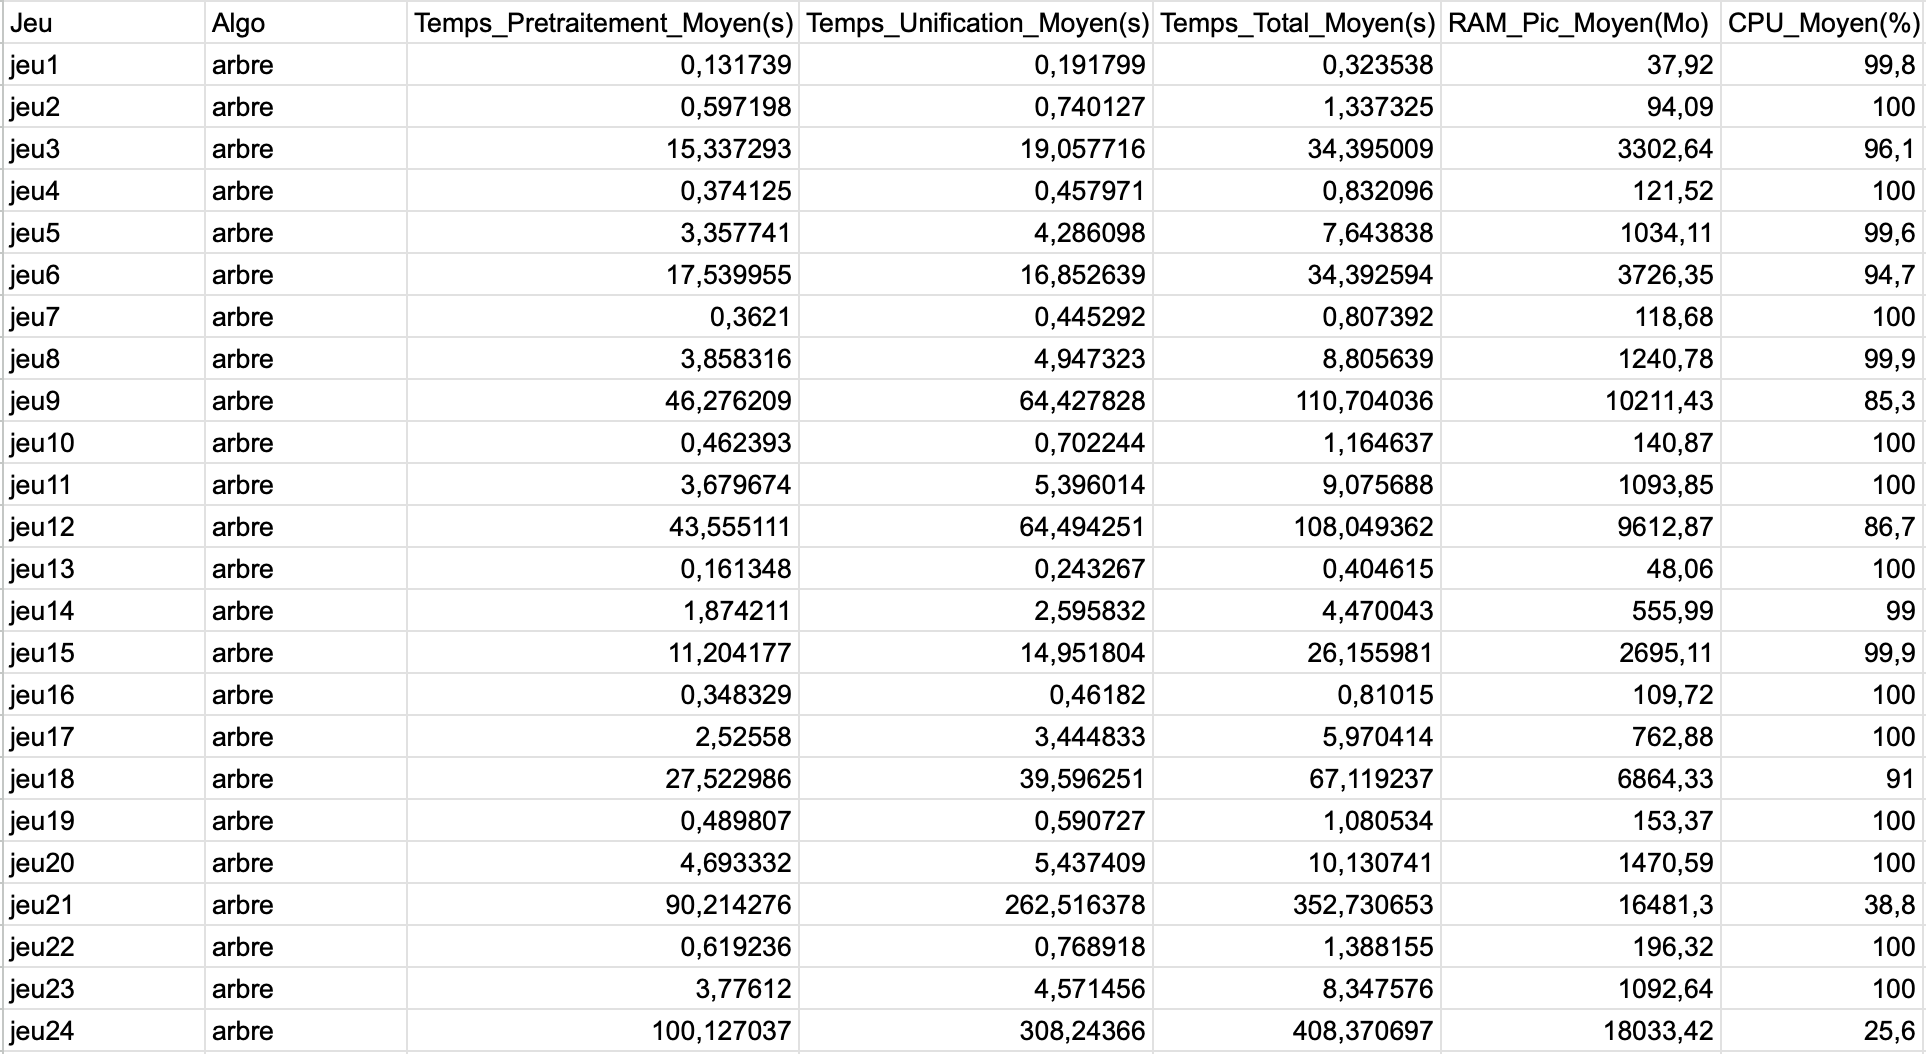
\includegraphics[width=0.8\textwidth]{img/bench/arbre_TRUE.png}
    \caption{Arbre de discrimination pour toutes les unifications}
    \label{fig:arbre TRUE}
\end{figure}

\begin{figure}[H]
    \centering
    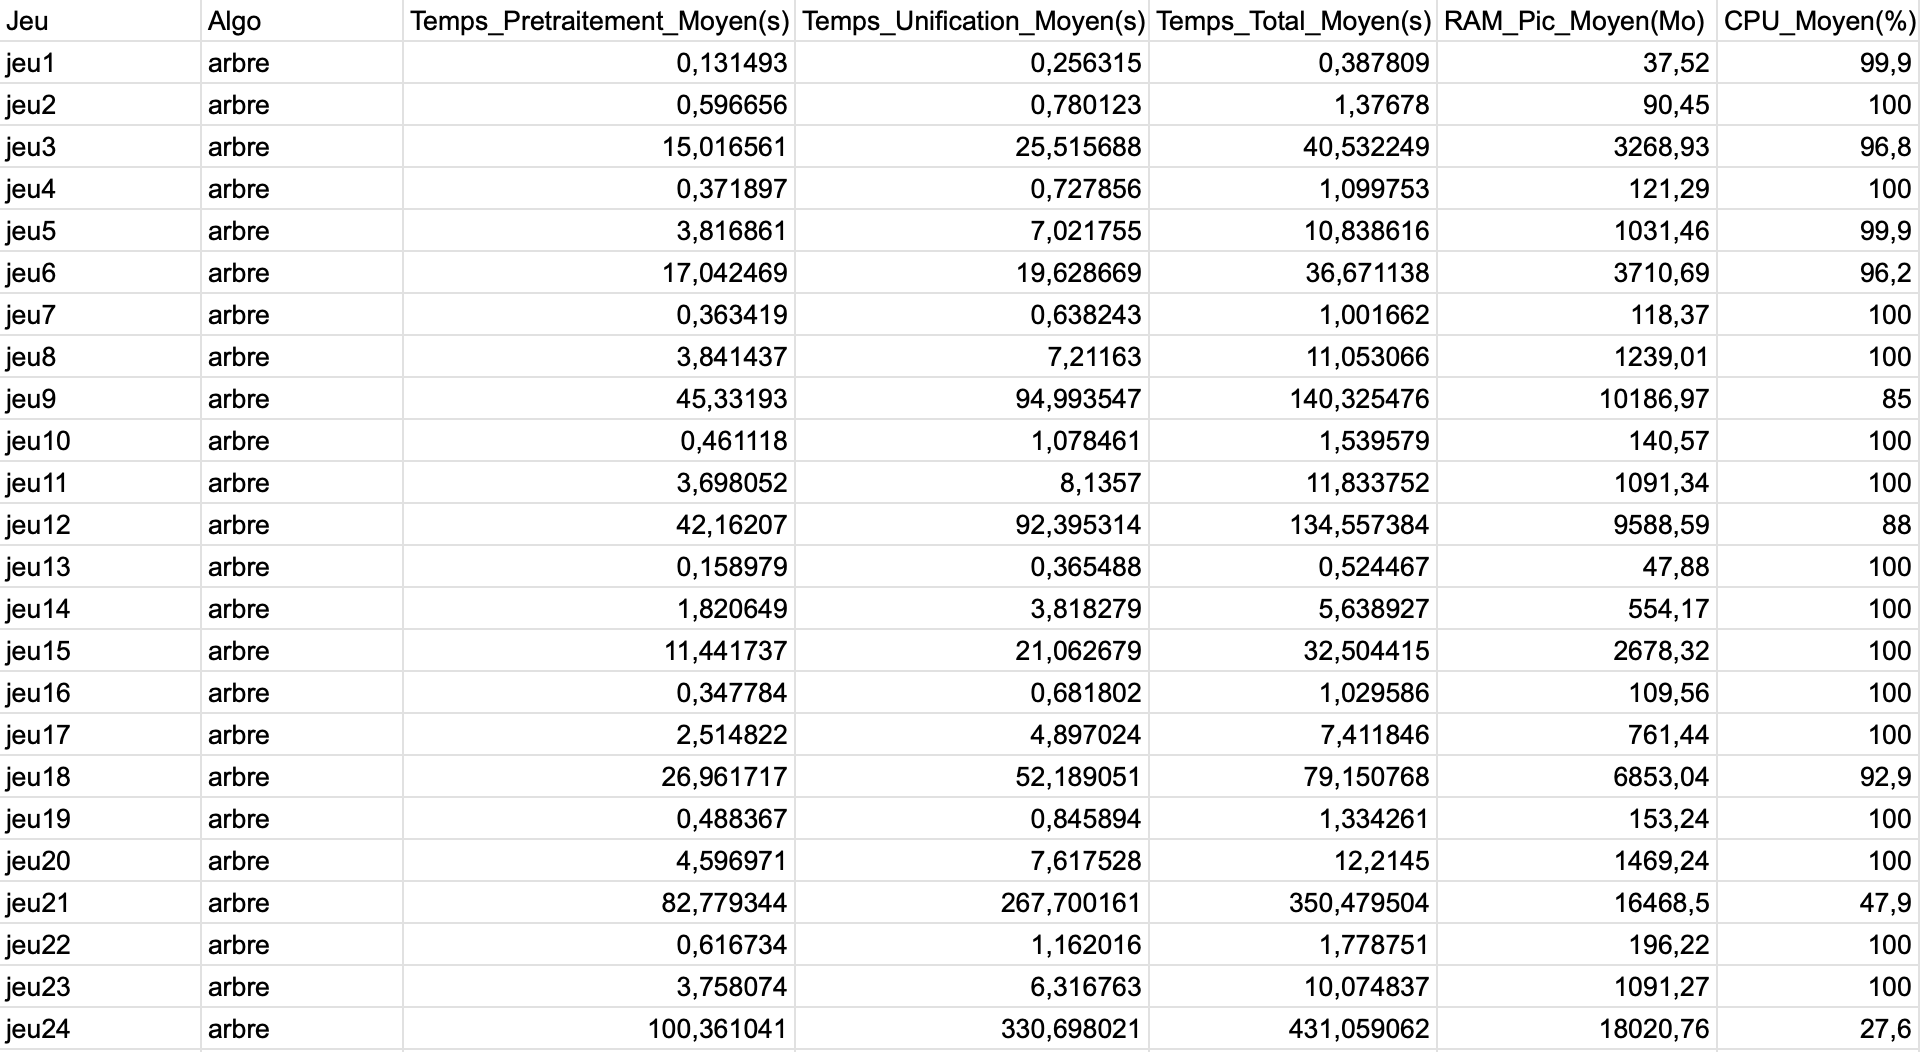
\includegraphics[width=0.8\textwidth]{img/bench/arbre_FALSE.png}
    \caption{Arbre de discrimination pour la première unification}
    \label{fig:arbre FALSE}
\end{figure}

\section{Résultats de l'algorithme de Robinson}
\label{annexe:Robinson}

\begin{figure}[H]
    \centering
    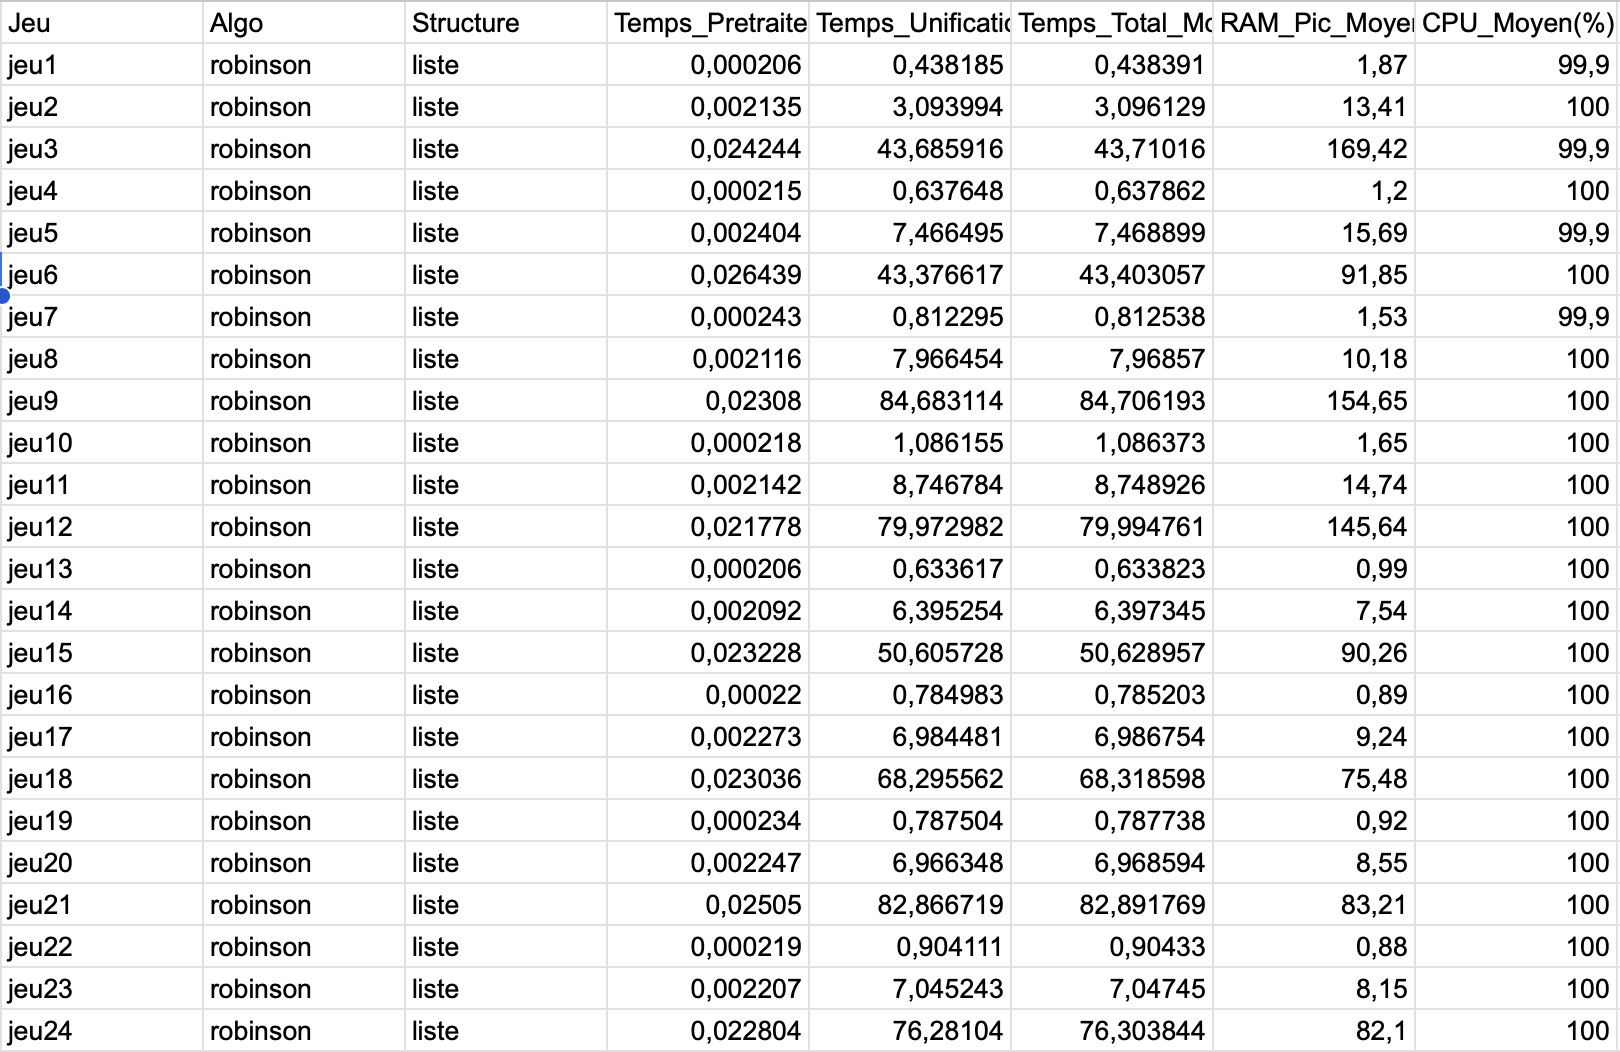
\includegraphics[width=0.8\textwidth]{img/bench/rob_liste_TRUE.png}
    \caption{Robinson pour toutes les unifications}
    \label{fig:rob liste TRUE}
\end{figure}

\begin{figure}[H]
    \centering
    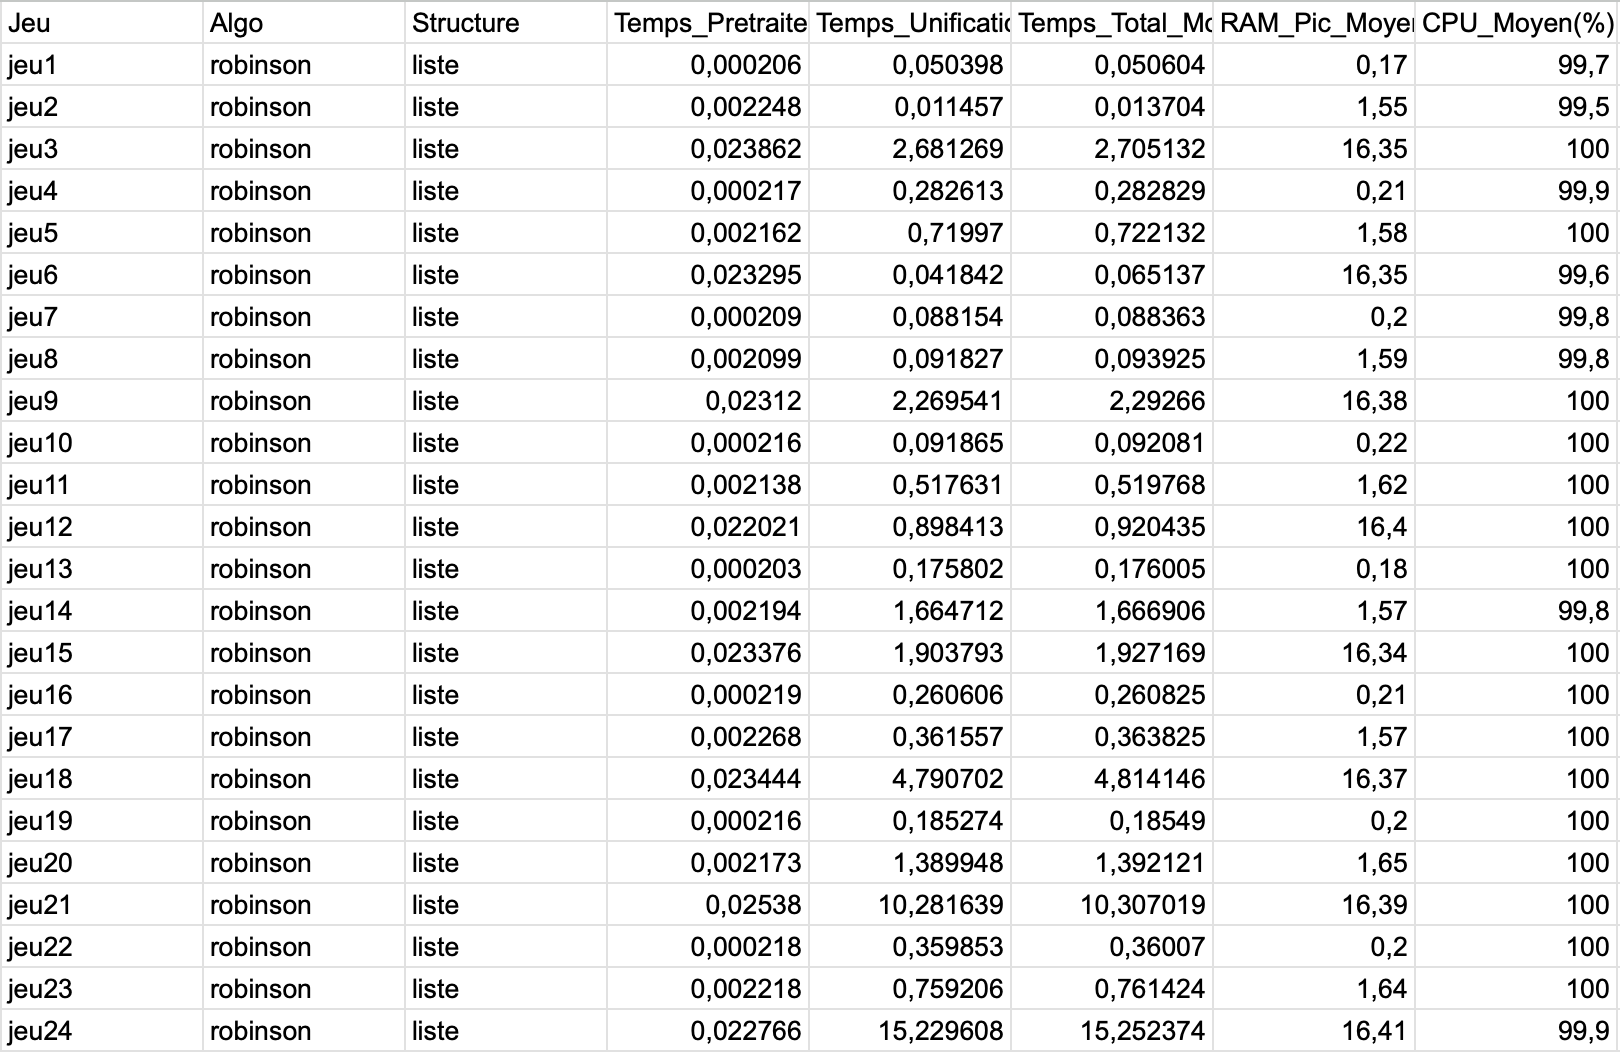
\includegraphics[width=0.8\textwidth]{img/bench/rob_liste_FALSE.png}
    \caption{Robinson (Liste) pour la première unification}
    \label{fig:rob liste FALSE}
\end{figure}

\begin{figure}[H]
    \centering
    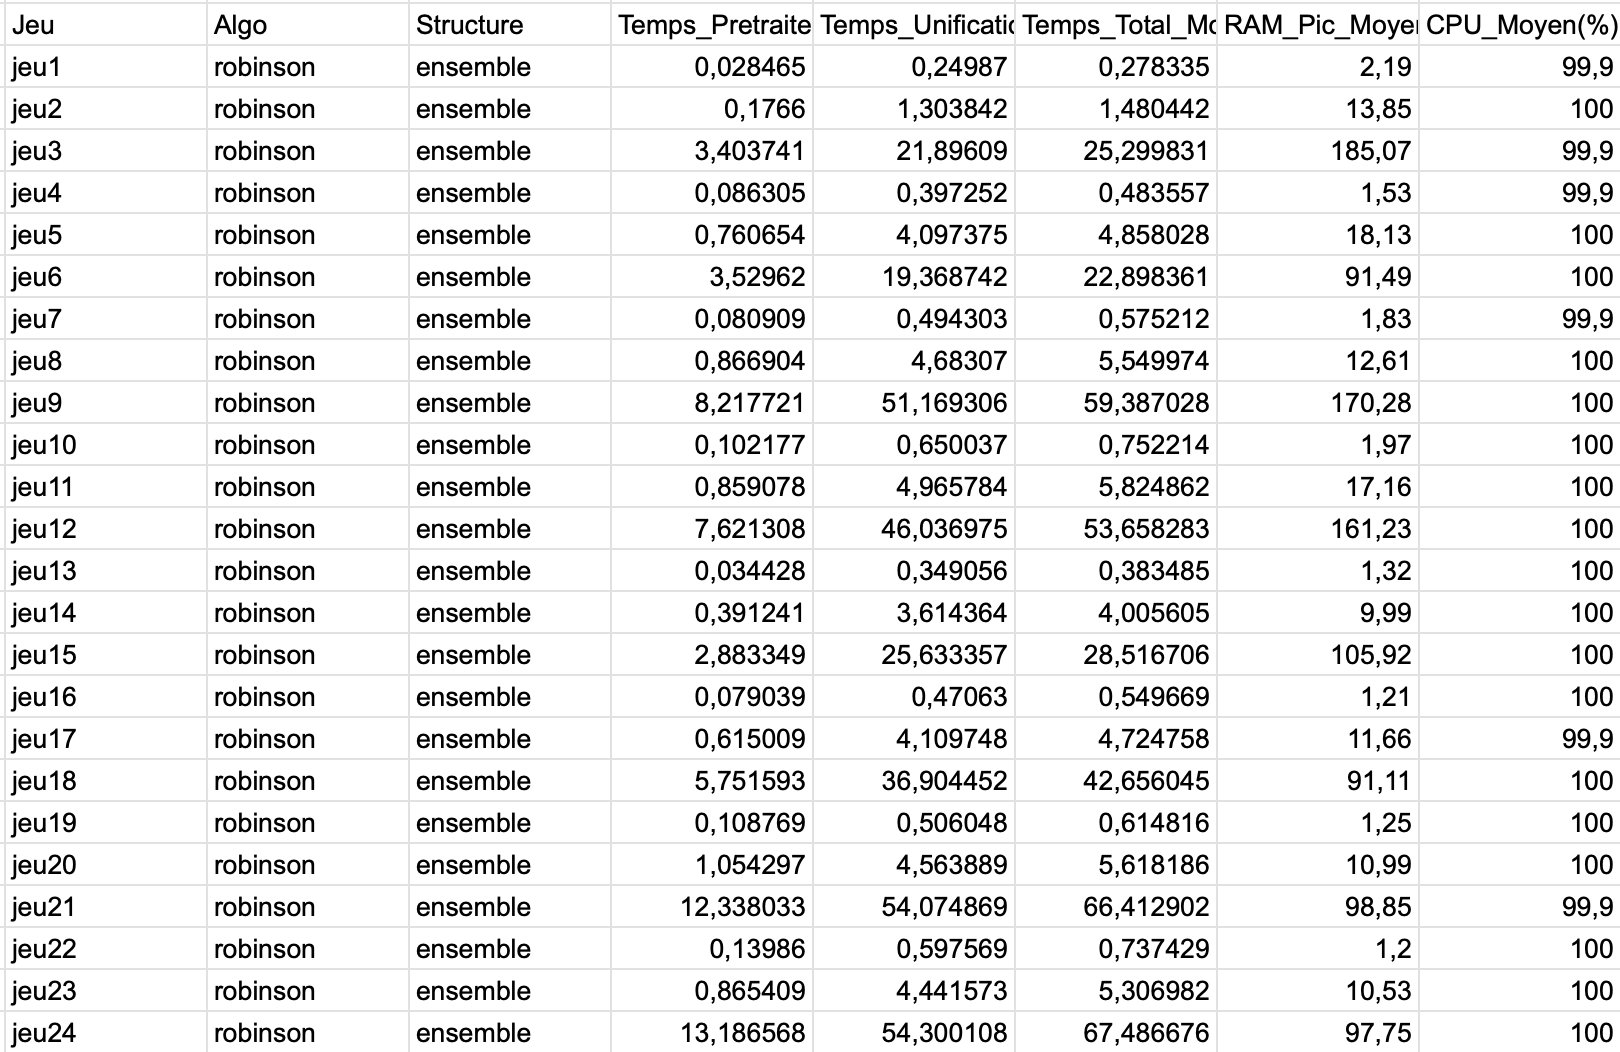
\includegraphics[width=0.8\textwidth]{img/bench/rob_ensemble_TRUE.png}
    \caption{Robinson (Ensemble) pour toutes les unifications}
    \label{fig:rob ensemble TRUE}
\end{figure}

\begin{figure}[H]
    \centering
    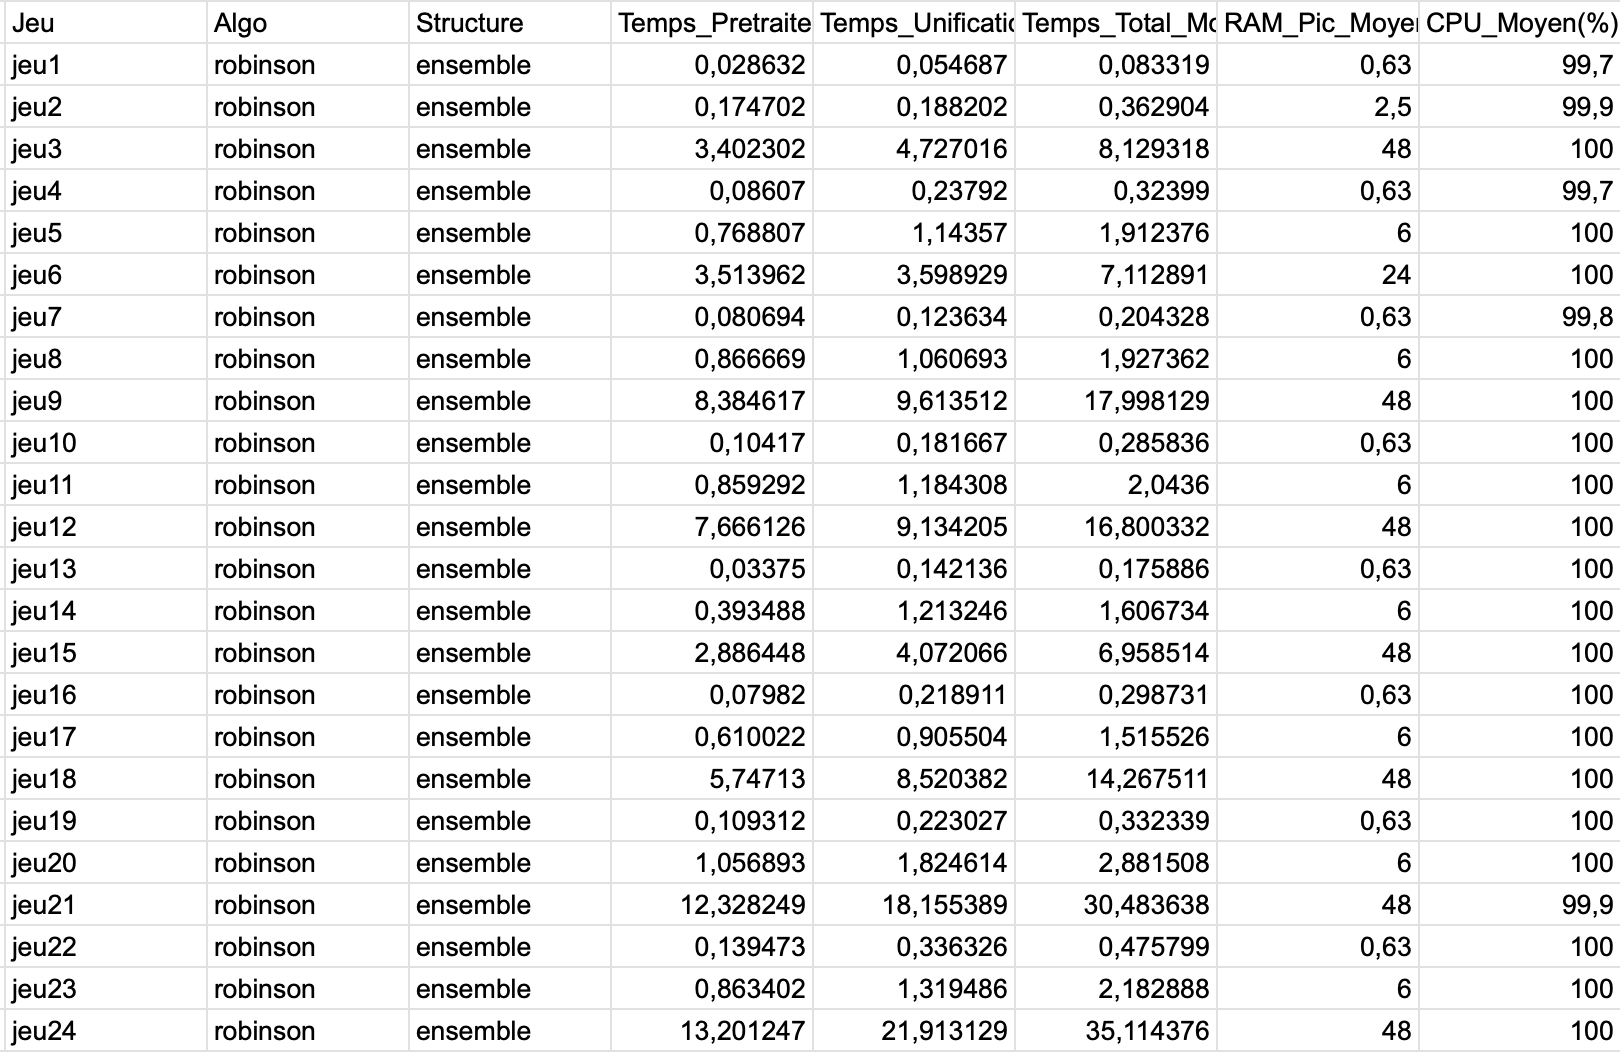
\includegraphics[width=0.8\textwidth]{img/bench/rob_ensemble_FALSE.png}
    \caption{Robinson (Ensemble) pour la première unification}
    \label{fig:rob ensemble FALSE}
\end{figure}

\begin{figure}[H]
    \centering
    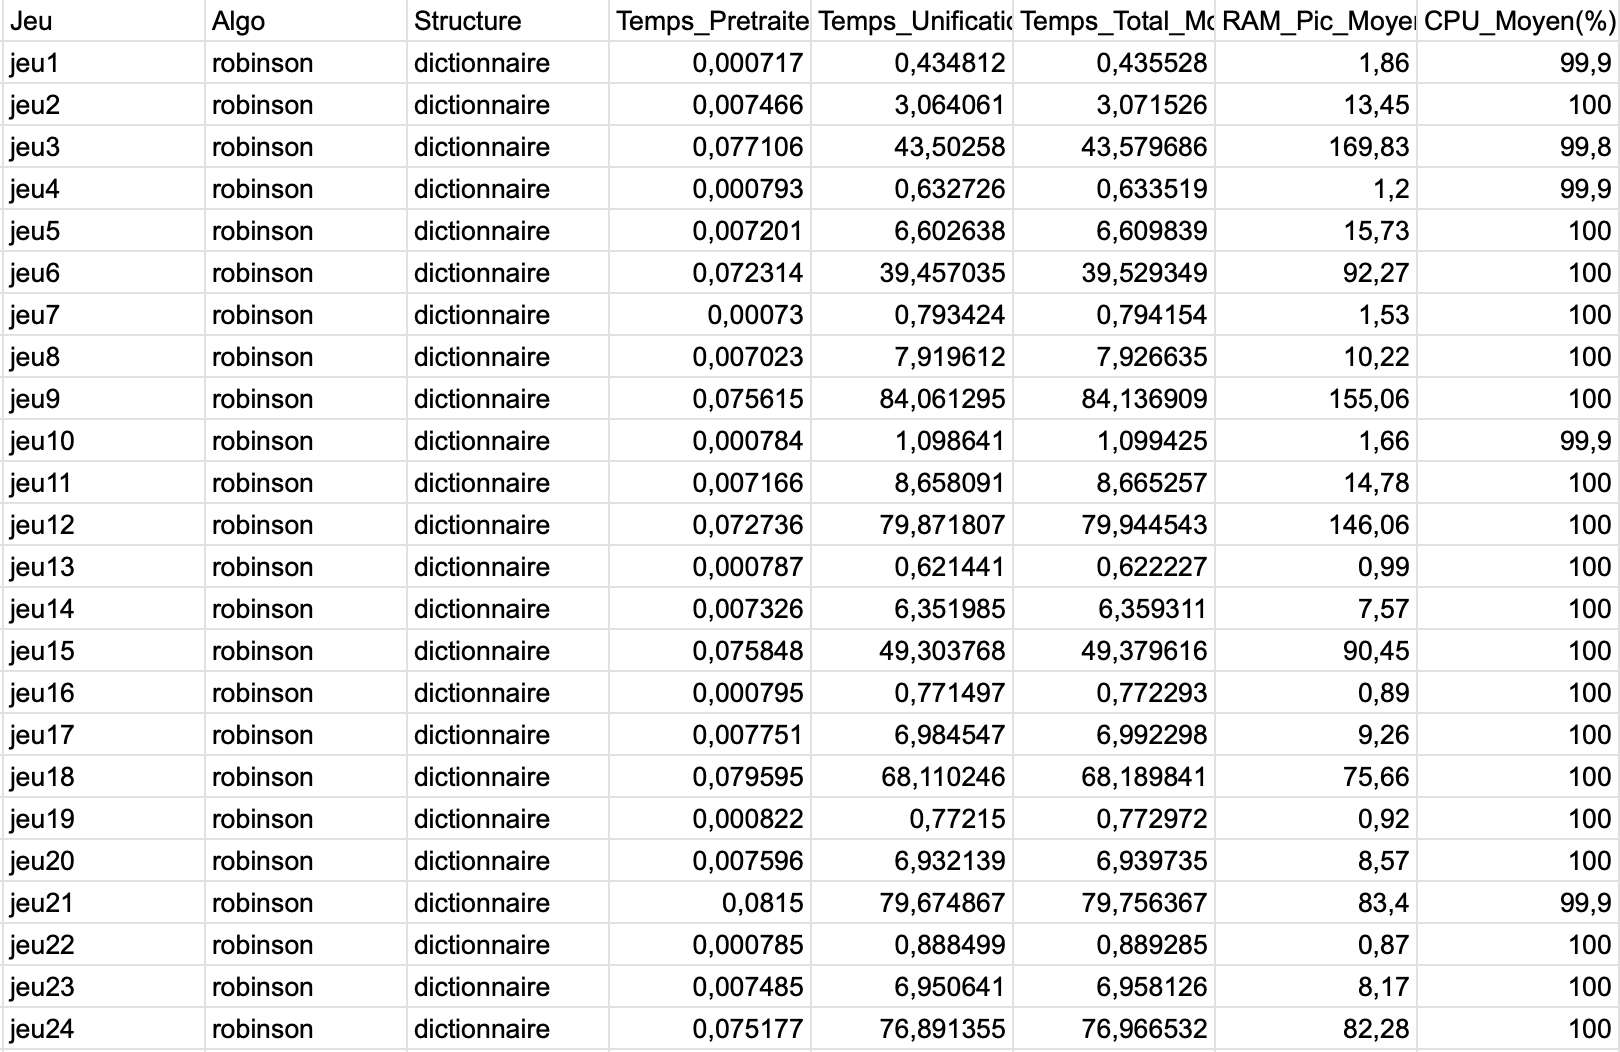
\includegraphics[width=0.8\textwidth]{img/bench/rob_dictionnaire_TRUE.png}
    \caption{Robinson (Dictionnaire) pour toutes les unifications}
    \label{fig:rob dictionnaire TRUE}
\end{figure}

\begin{figure}[H]
    \centering
    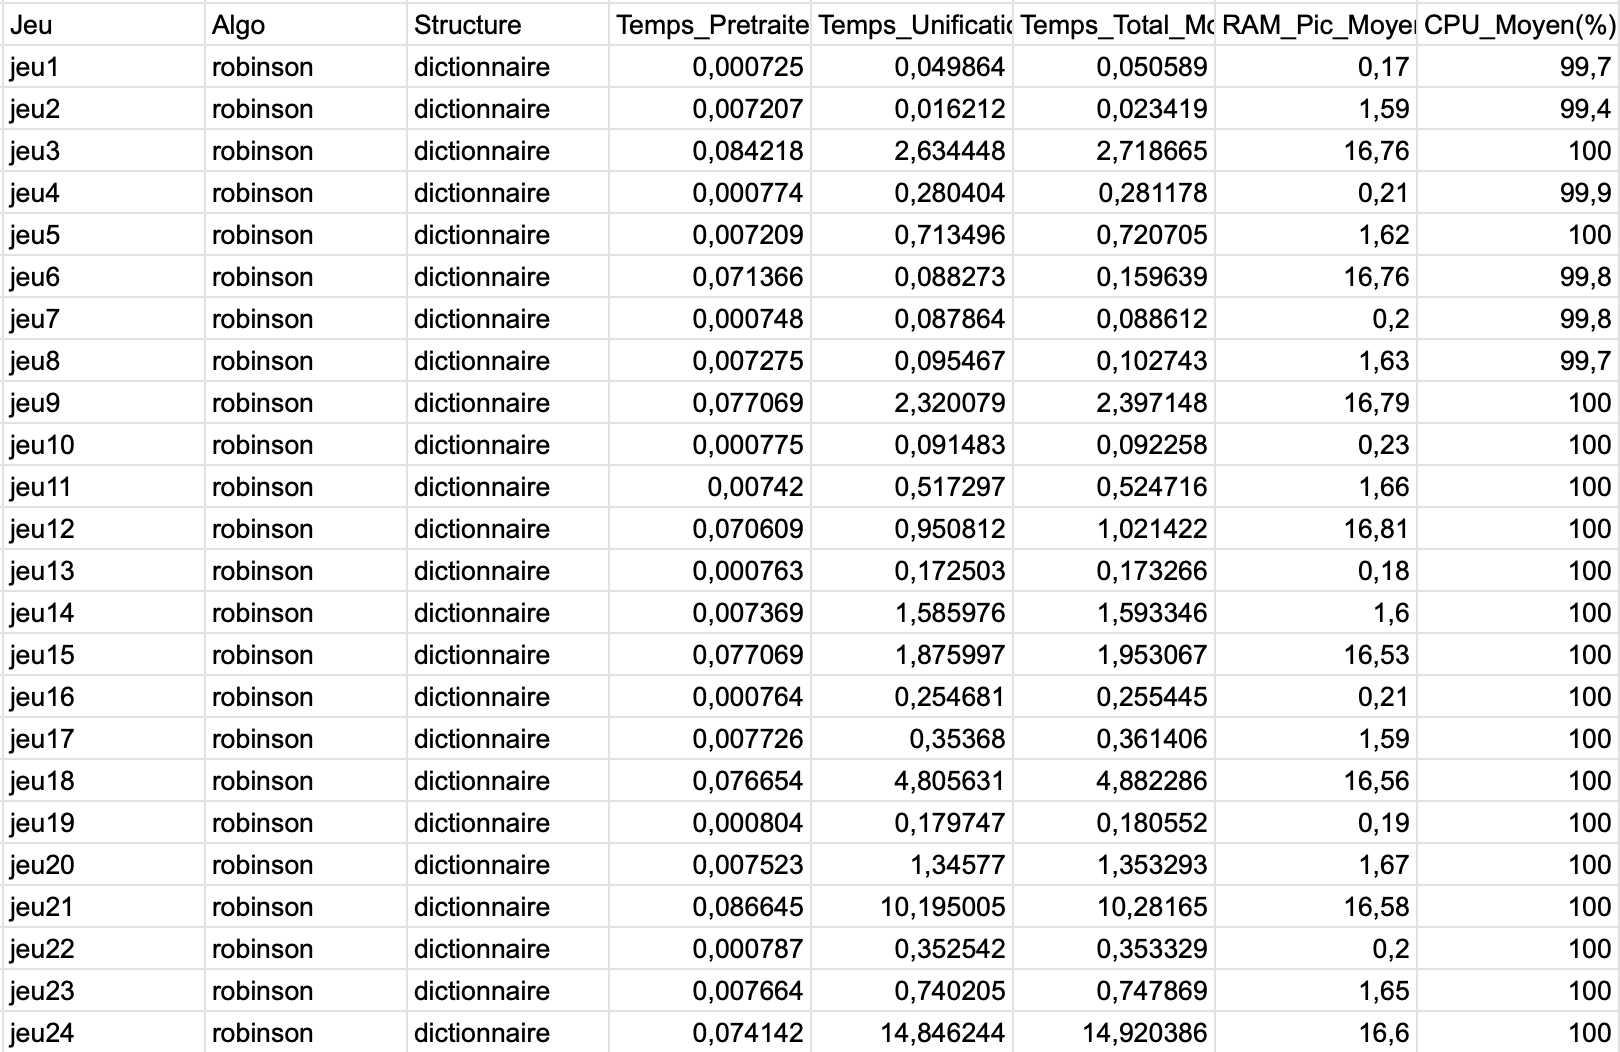
\includegraphics[width=0.8\textwidth]{img/bench/rob_dictionnaire_FALSE.png}
    \caption{Robinson (Dictionnaire) pour la première unification}
    \label{fig:rob dictionnaire FALSE}
\end{figure}


\section{Résultats de l'algorithme Martelli-Montanari}
\label{annexe:MM}

\begin{figure}[H]
    \centering
    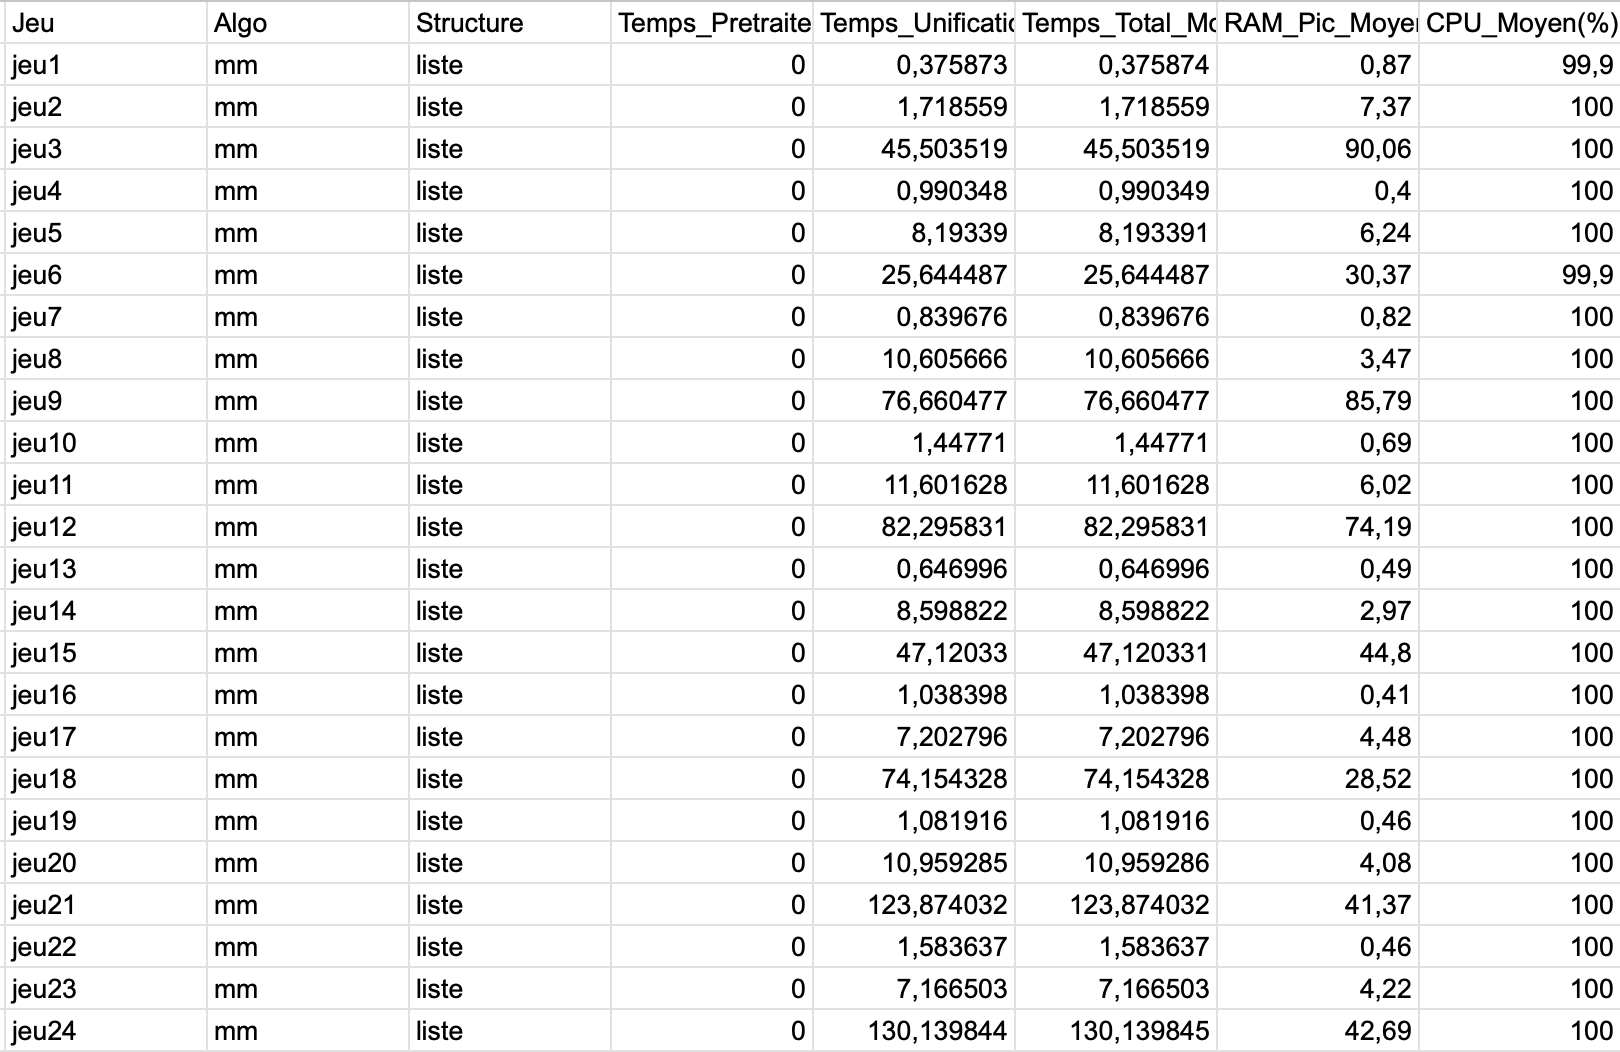
\includegraphics[width=0.8\textwidth]{img/bench/mm_liste_TRUE.png}
    \caption{Martelli-Montanari (Liste) pour toutes les unifications}
    \label{fig:mm liste TRUE}
\end{figure}

\begin{figure}[H]
    \centering
    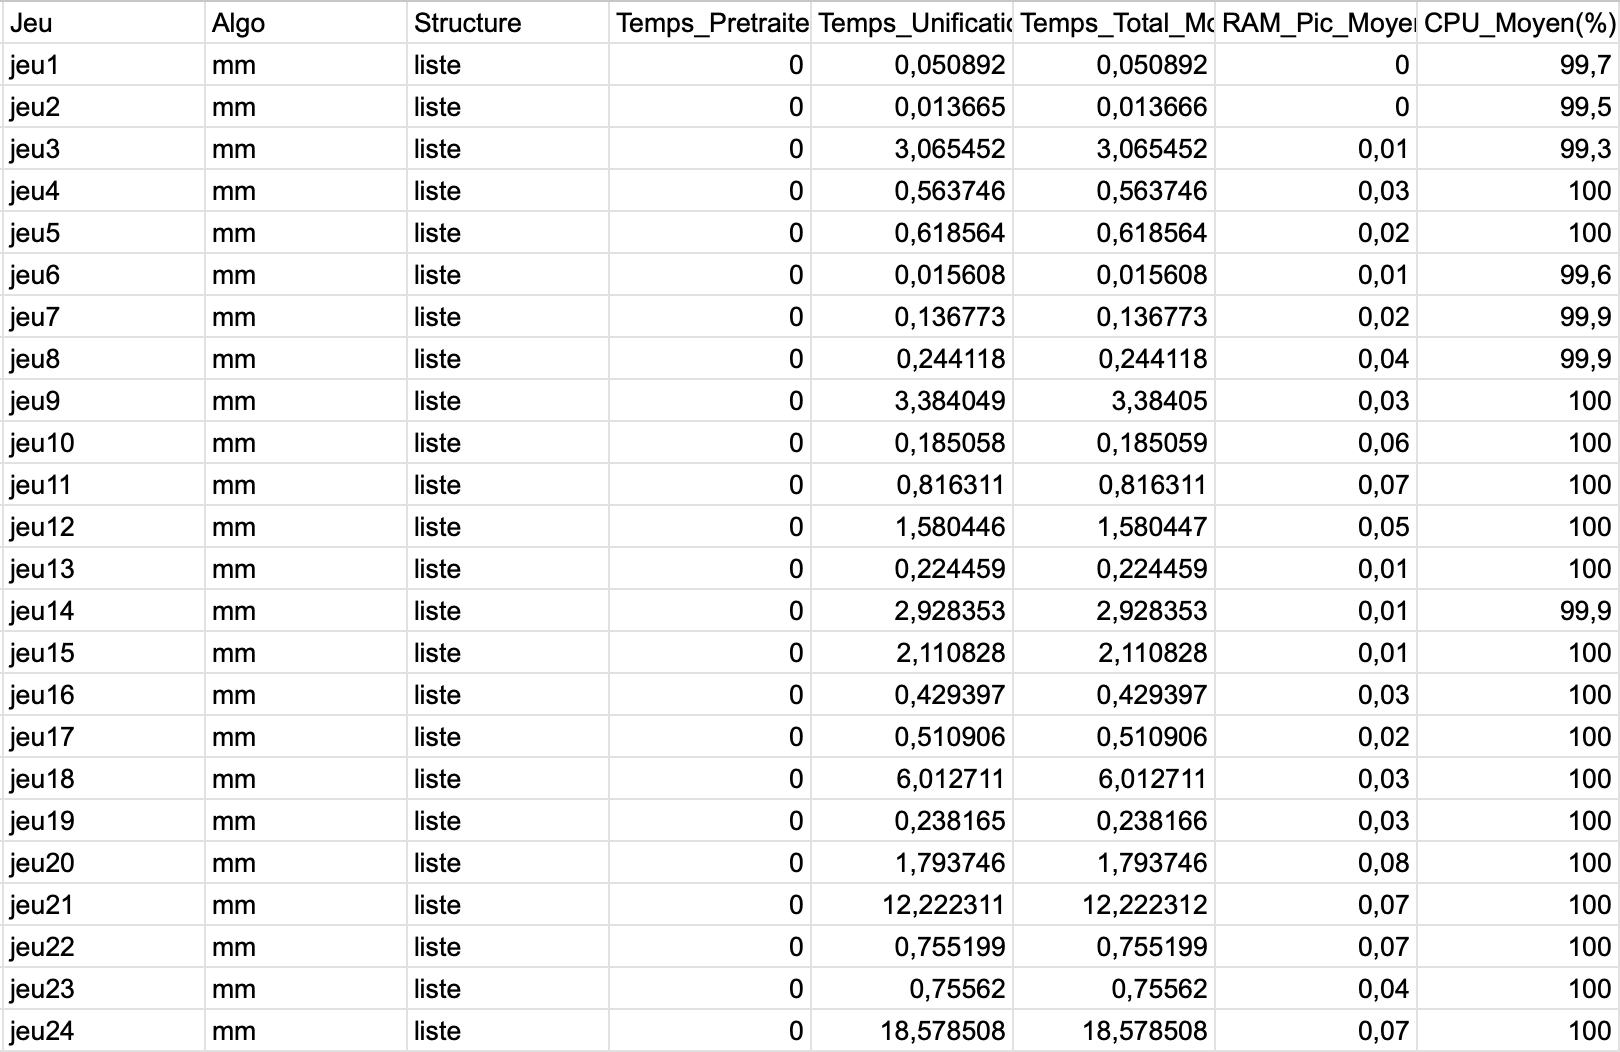
\includegraphics[width=0.8\textwidth]{img/bench/mm_liste_FALSE.png}
    \caption{Martelli-Montanari (Liste) pour la première unification}
    \label{fig:mm liste FALSE}
\end{figure}

\begin{figure}[H]
    \centering
    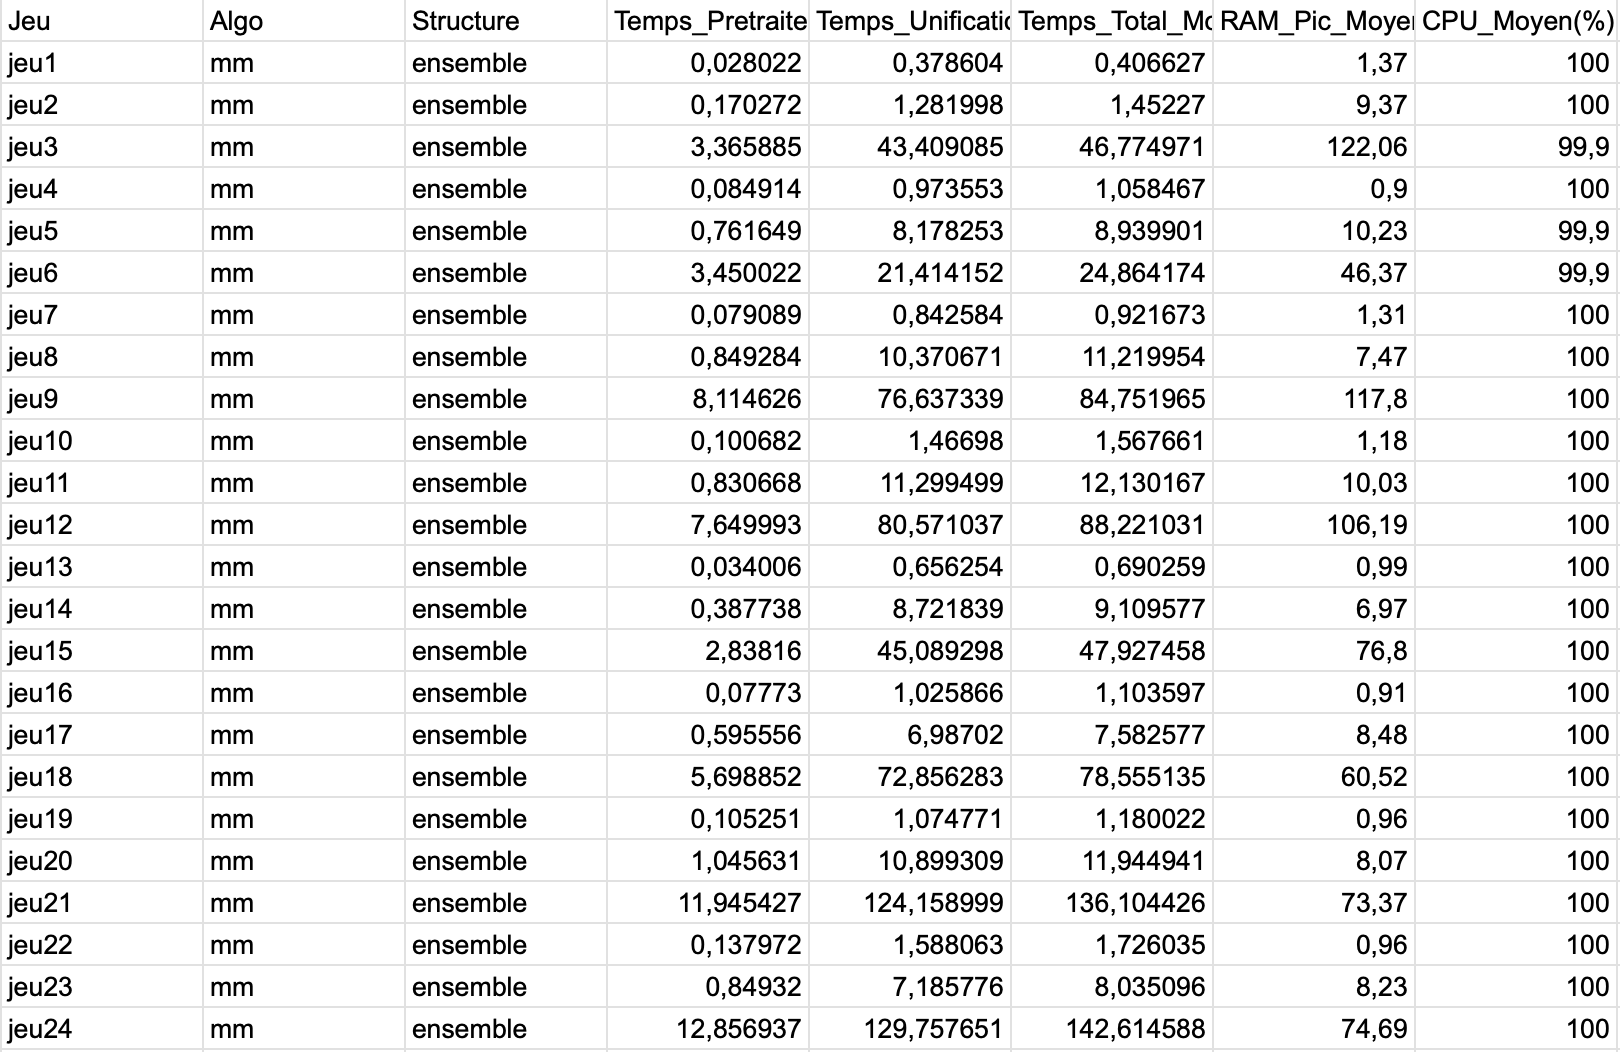
\includegraphics[width=0.8\textwidth]{img/bench/mm_ensemble_TRUE.png}
    \caption{Martelli-Montanari (Ensemble) pour toutes les unifications}
    \label{fig:mm ensemble TRUE}
\end{figure}

\begin{figure}[H]
    \centering
    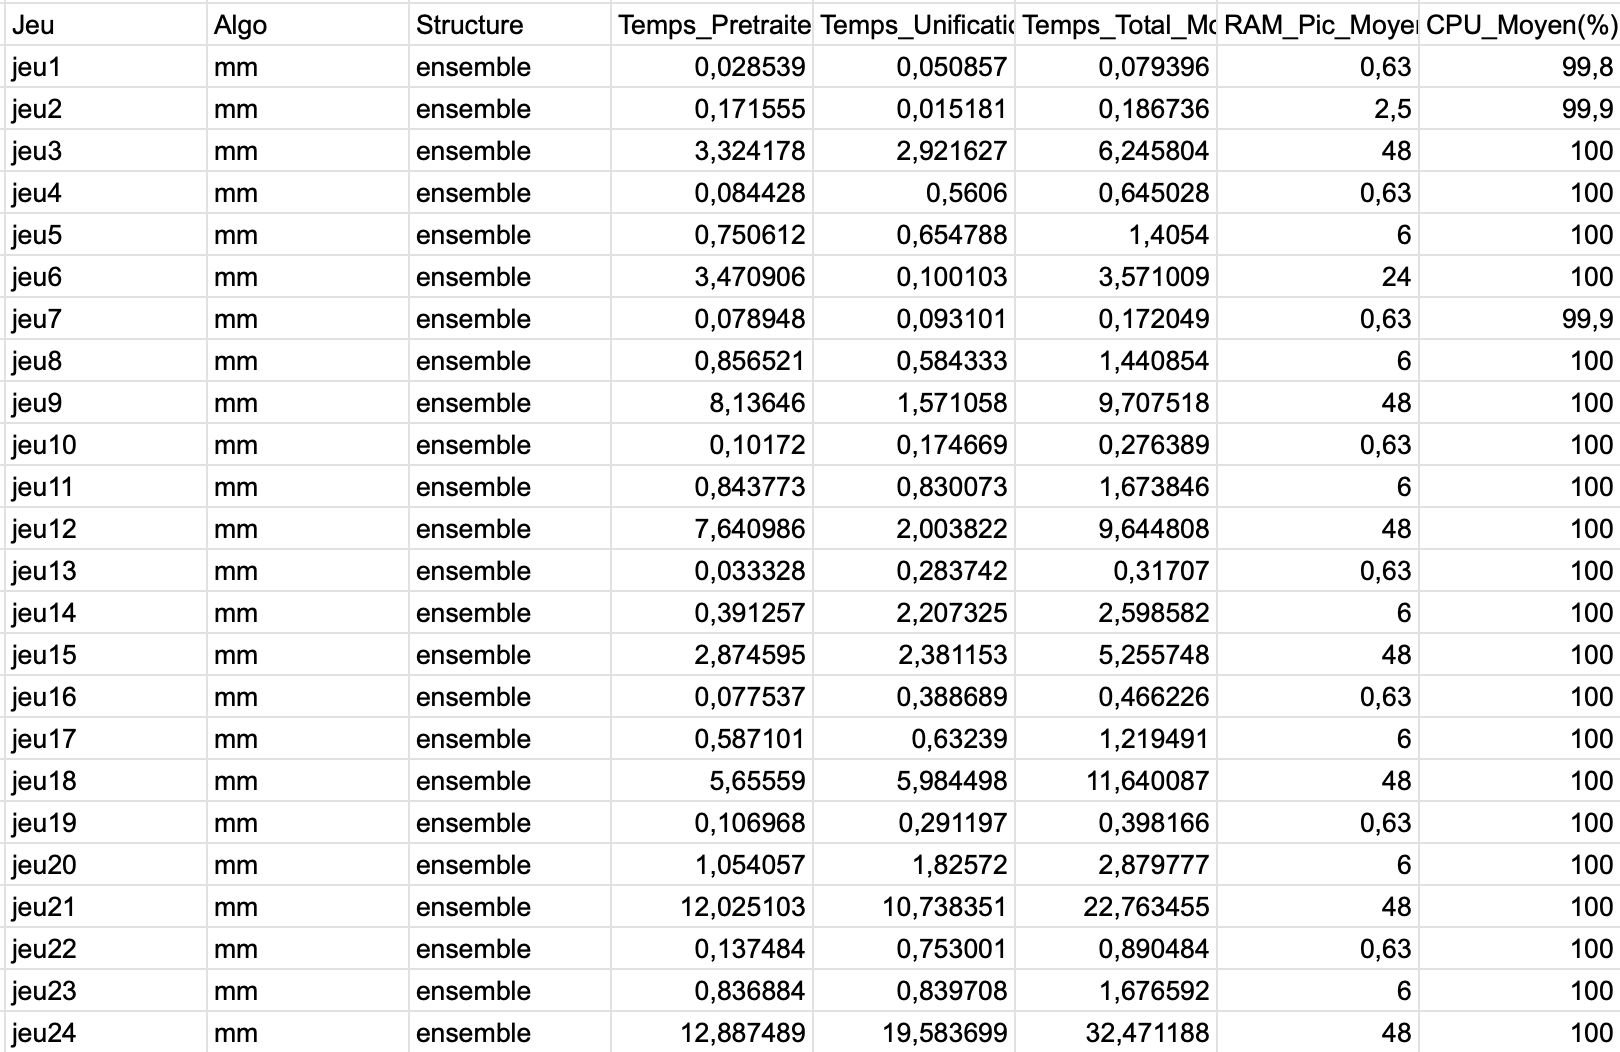
\includegraphics[width=0.8\textwidth]{img/bench/mm_ensemble_FALSE.png}
    \caption{Martelli-Montanari (Ensemble) pour la première unification}
    \label{fig:mm ensemble FALSE}
\end{figure}

\begin{figure}[H]
    \centering
    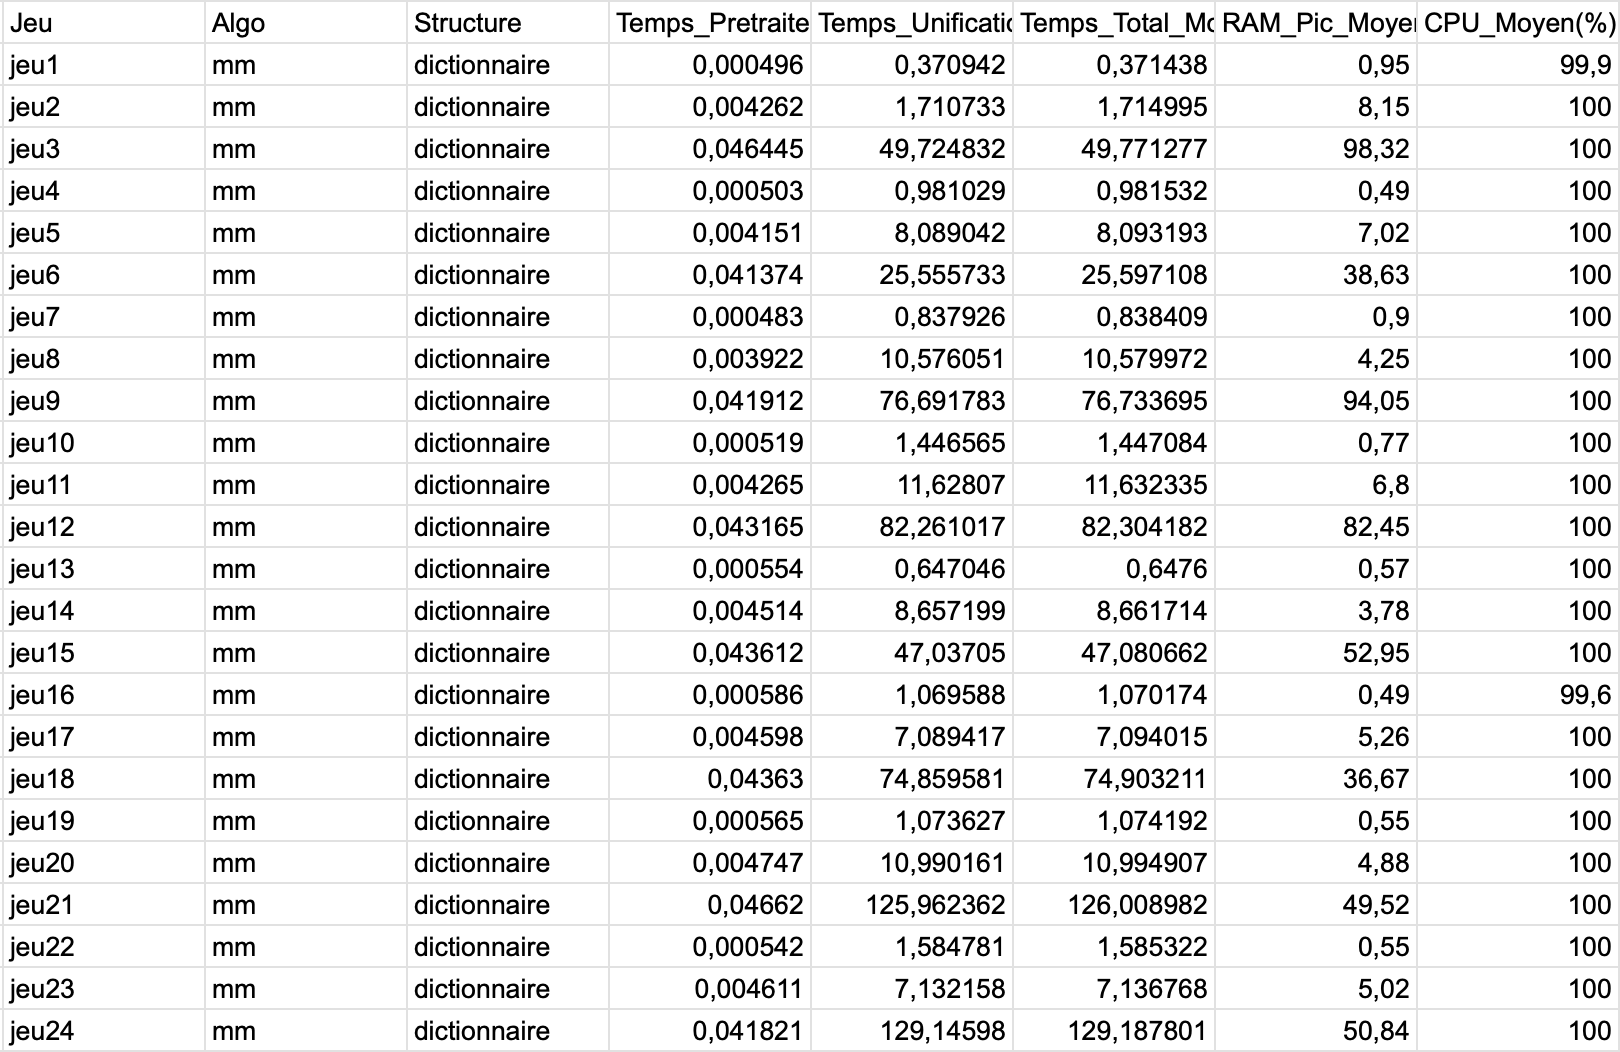
\includegraphics[width=0.8\textwidth]{img/bench/mm_dictionnaire_TRUE.png}
    \caption{Martelli-Montanari (Dictionnaire) pour toutes les unifications}
    \label{fig:mm dictionnaire TRUE}
\end{figure}

\begin{figure}[H]
    \centering
    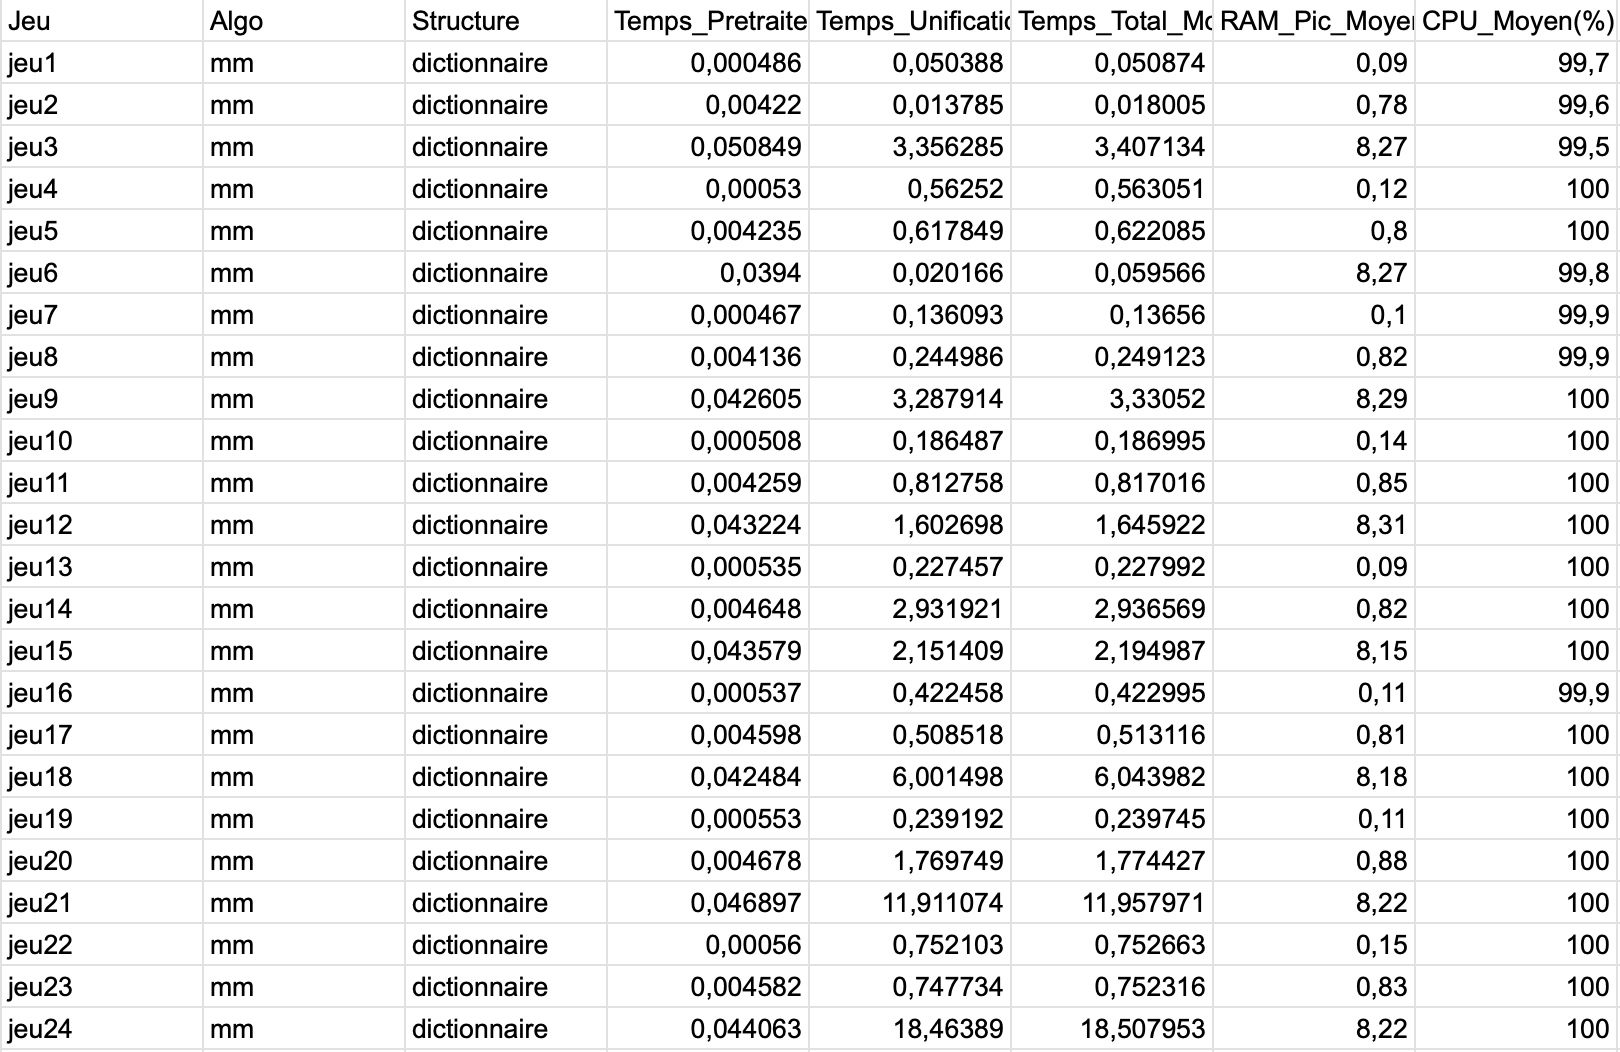
\includegraphics[width=0.8\textwidth]{img/bench/mm_dictionnaire_FALSE.png}
    \caption{Martelli-Montanari (Dictionnaire) pour la première unification}
    \label{fig:mm dictionnaire FALSE}
\end{figure}

\section{Graphiques}
\label{annexe:graphiques}

\begin{figure}[H]
    \centering
    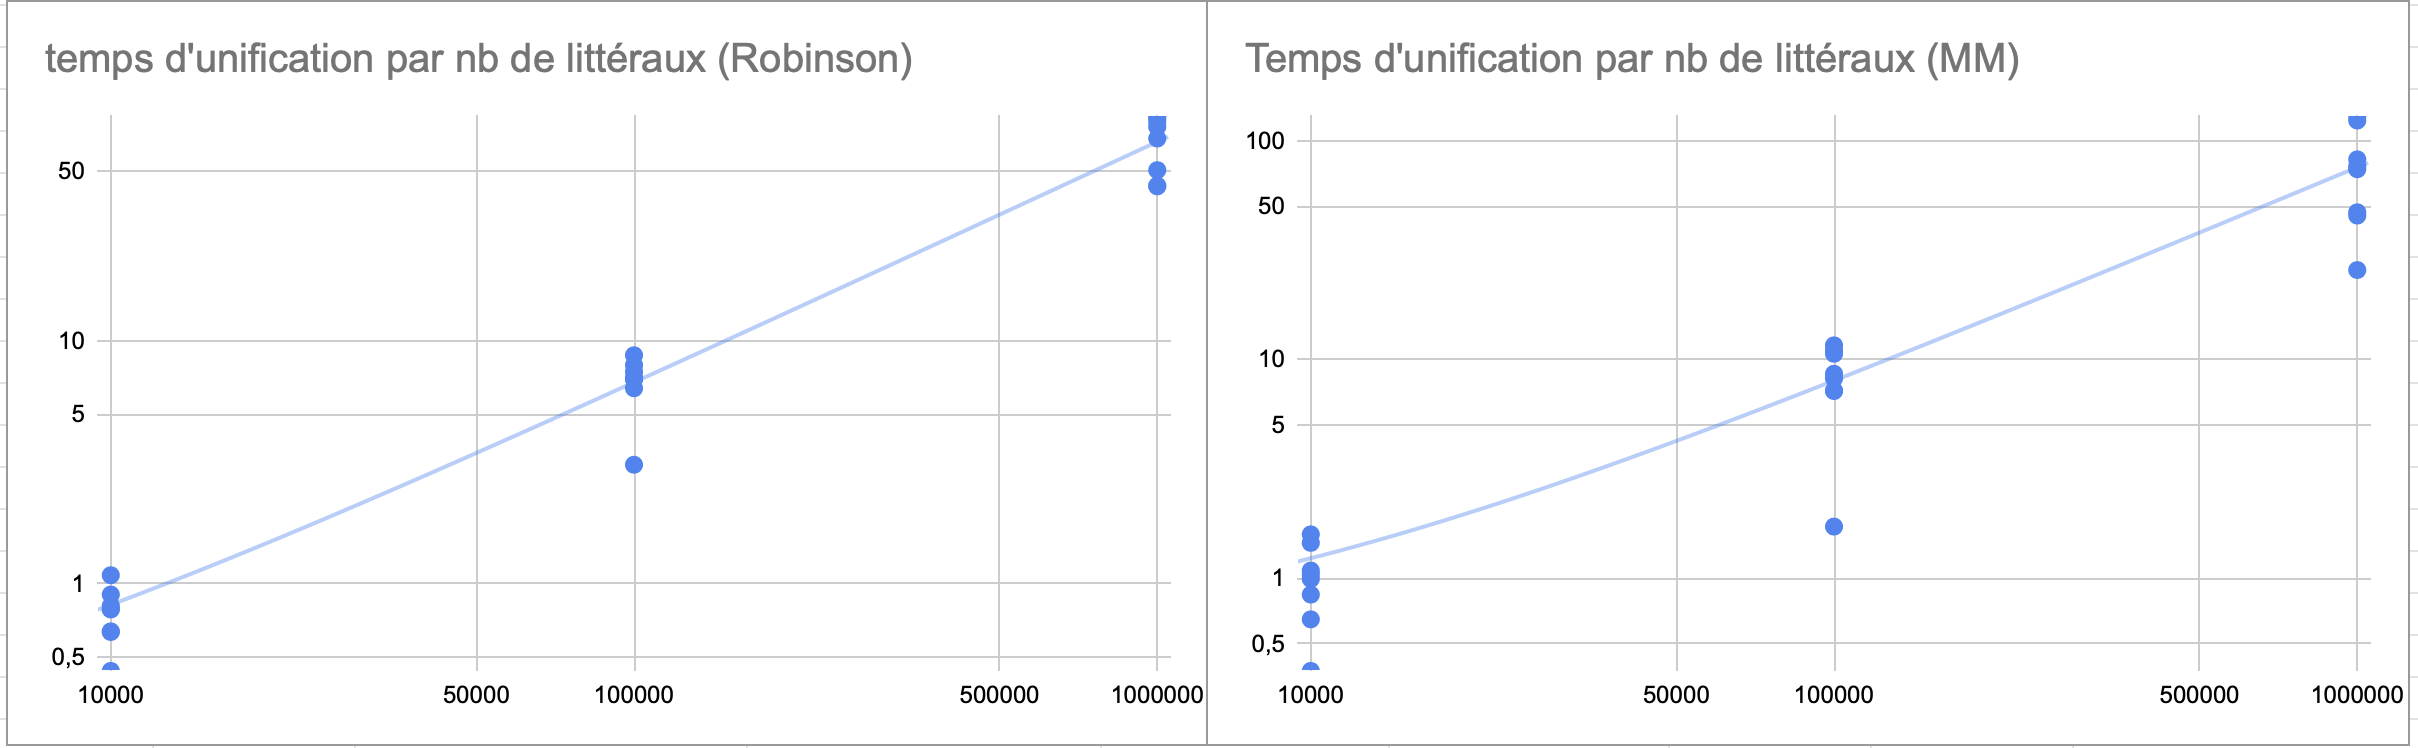
\includegraphics[width=0.8\textwidth]{img/bench/tpsUnif_nb_lit_rob_et_MM.png}
    \caption{Temps d'unification par nombre de littéraux pour Robinson (à gauche) et MM (à droite) \\ Un point bleu correspond à un jeu de test }
\end{figure}

\begin{figure}[H]
    \centering
    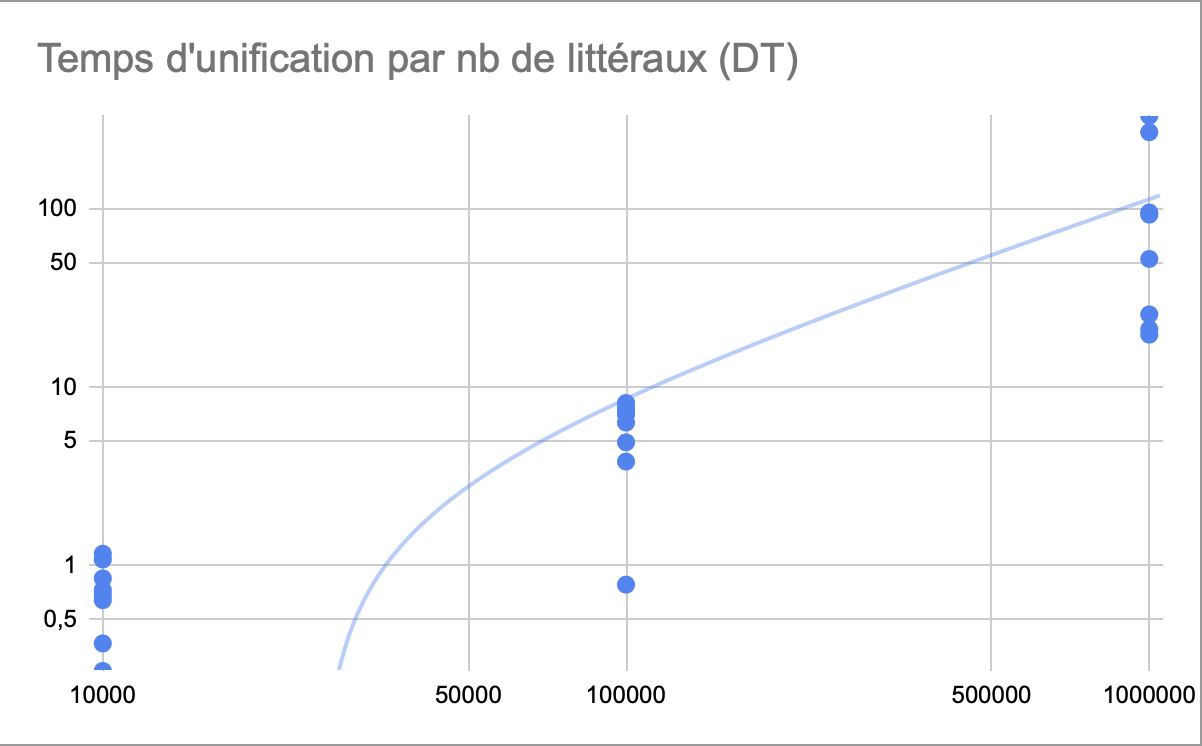
\includegraphics[width=0.8\textwidth]{img/bench/tpsUnif_nb_lit_DT.png}
    \caption{Temps d'unification par nombre de littéraux pour l'arbre de discrimination \\ Un point bleu correspond à un jeu de test }
\end{figure}

\begin{figure}[H]
    \centering
    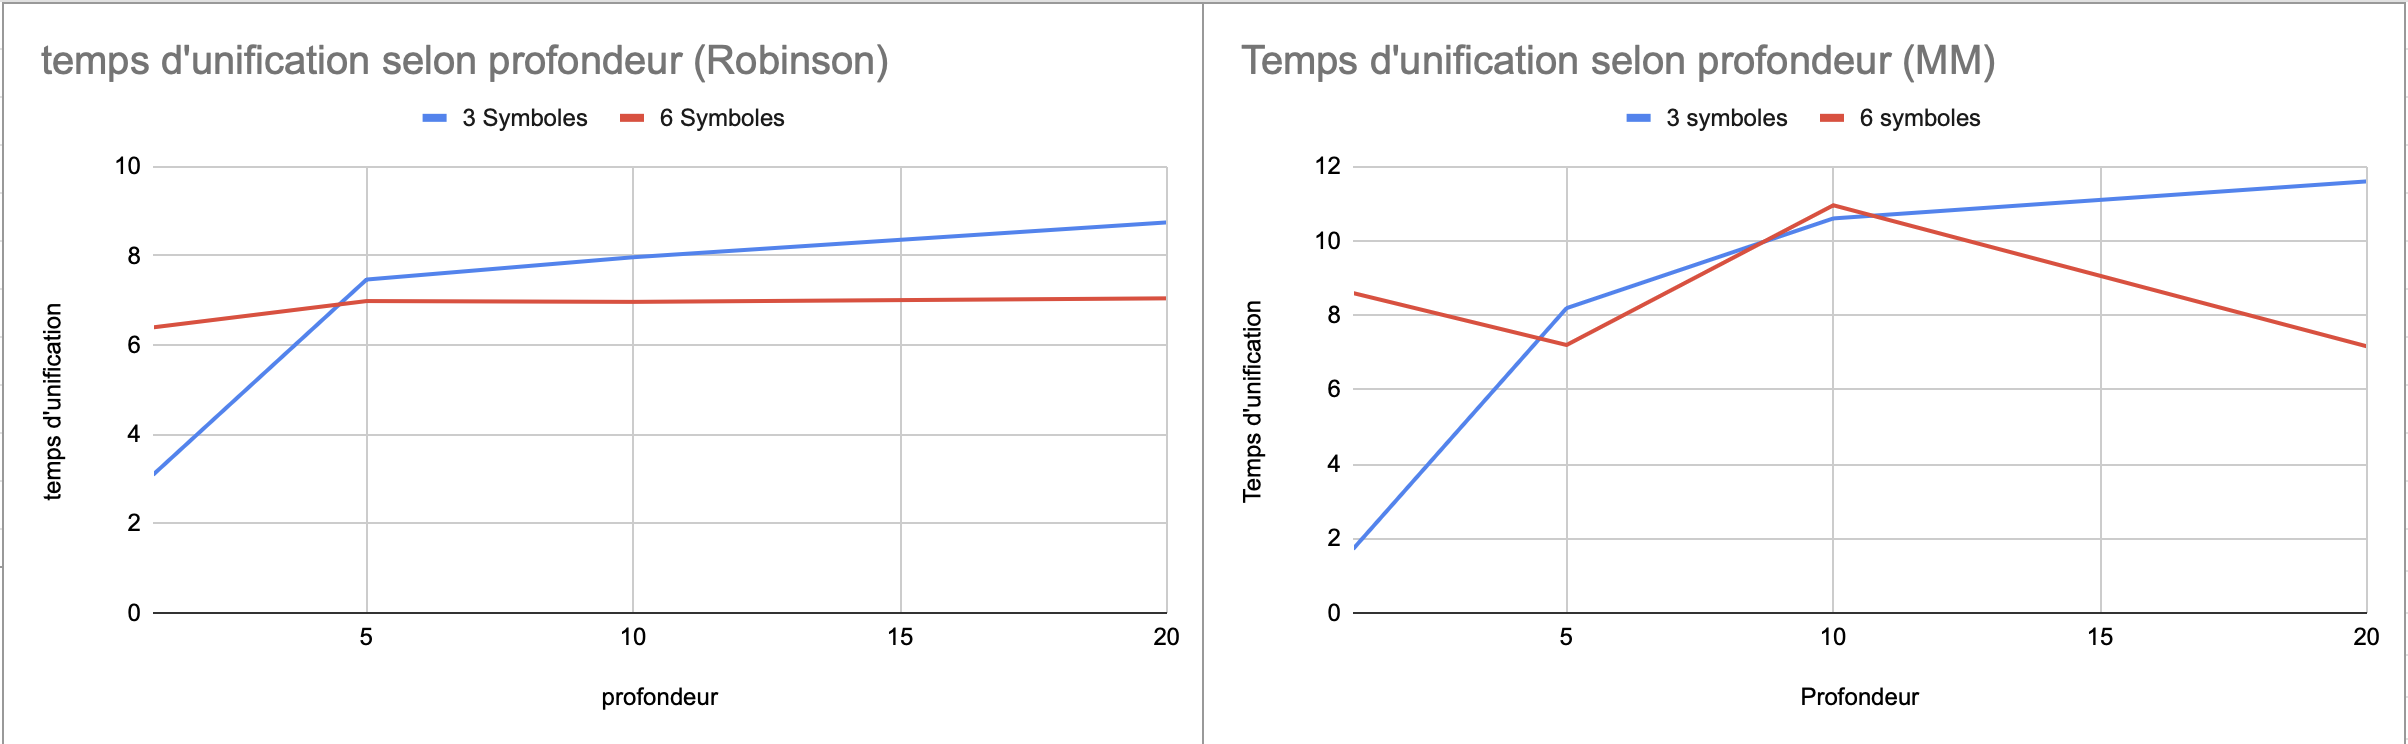
\includegraphics[width=0.8\textwidth]{img/bench/tpsUnif_prof_rob_et_MM.png}
    \caption{Temps d'unification en fonction de la profondeur des données de Robinson (à gauche) et MM (à droite) \\ Une courbe correspond à un nombre de symbole de prédicats donné }
\end{figure}

\begin{figure}[H]
    \centering
    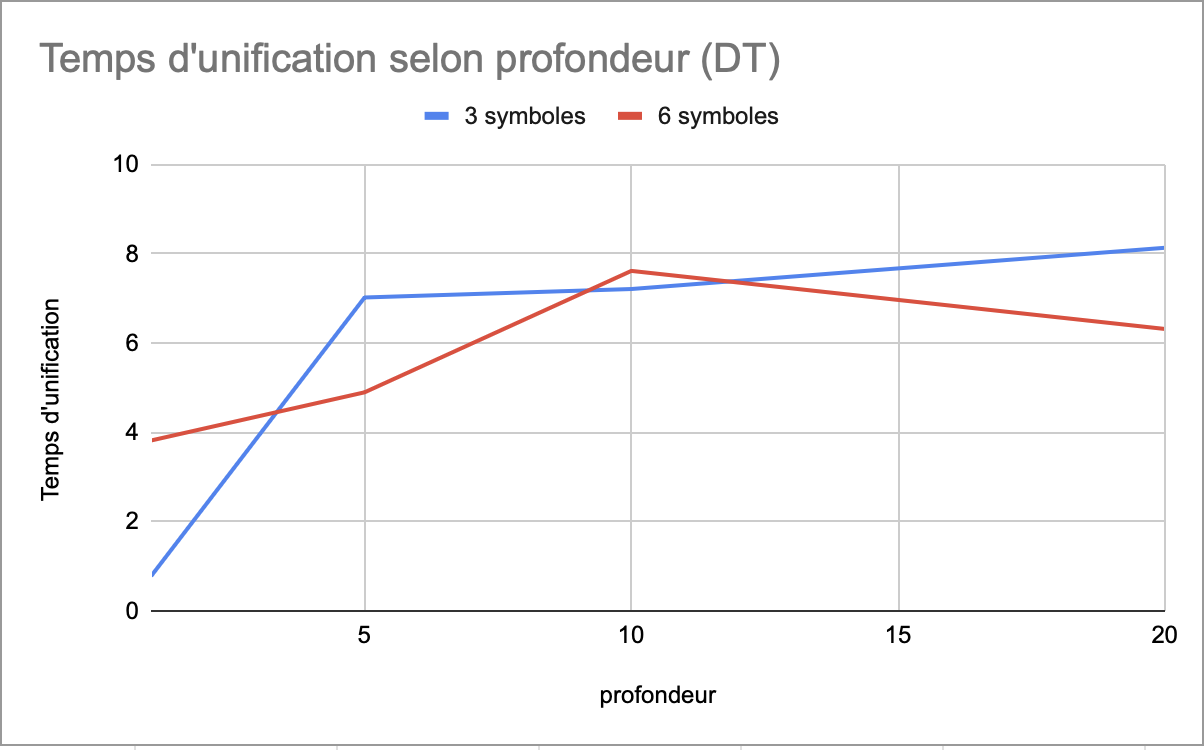
\includegraphics[width=0.8\textwidth]{img/bench/tpsUnif_prof_DT.png}
    \caption{Temps d'unification en fonction de la profondeur des données de l'arbre de discrimination \\ Une courbe correspond à un nombre de symbole de prédicats donné }
\end{figure}

\newpage

% --- Bibliographie --- %
\printbibliography

\end{document}